\chapter{Introduction}
\label{chap:introduction}

\section{Motivation}
\label{sec:motivation}
Large Language Models (LLMs) have been widely studied and applied to question-answering tasks across different domains, including finance \citep{sarmah2024hybridrag}, medicine \citep{wang2024llmhealthcare}, law \citep{lai2024llmlaw}, and scientific discovery \citep{zhang2024scientificllm}. For knowledge-intensive tasks, Retrieval-Augmented Generation (RAG) is particularly useful because generation is supported by external evidence rather than relying solely on the model's internal knowledge \citep{lewis2020rag}. However, conventional RAG may be less effective for narrative-rich texts, because it tends to process information at the level of isolated documents or passages and can therefore overlook underlying event structures, temporal development and logical relationships between events \citep{yang2025eventrag}. Moreover, classical RAG is also limited for exhaustive and database-style queries such as \textit{find all battles satisfying condition X}. Such queries would require the RAG system to check this condition across the entire collection of documents, whereas RAG typically retrieves only a small top-$k$ subset of them. These limitations is particularly relevant to domains in which information is organized as complex narratives rather than isolated facts. Movies provide one such example, where adapting LLMs for narrative understanding remains an underexplored challenge \citep{shen2025narrative}. Historical battles represent another domain with rich event and narrative structure. A recent study has shown that simple quantitative statistics alone may fail to capture higher-level tactical patterns and similarities between battles \citep{coulson2023actionclusters}. Instead, meaningful similarities can emerge from the sequences and relationships between battle actions. This suggests that historical battles may benefit from richer representations that capture not only factual attributes but also the development and sequence of events.

In practice, many proprietary and open-weight models indeed struggle with database-style questions in complex narrative domains such as historical battles. As an example, we ask two well-known proprietary models, Gemini \citep{geminiteam2023gemini} and Claude \citep{anthropic2026claude}, several battle-related questions. It is especially interesting to see how these models are able to capture narrative-rich facts about less-known battles. First, we ask a model a question and prohibit any web search. If the model fails to mention relevant battles, we provide the gold labels and ask whether the model recognizes its mistake. Figure~\ref{fig:gemini_initial_response} and Figure~\ref{fig:gemini_followup_response} show the question asked to Gemini 3.6 Flash \citep{google2026gemini}. In this particular example, the model fails to mention two relevant battles, and after allowing it to use web search and explicitly asking about the missing battles, the model recognizes its mistake. Figures~\ref{fig:claude_initial_response} and~\ref{fig:claude_followup_response} demonstrate an analogous example with Claude Sonnet 5.5  \citep{anthropic2026sonnet55}. The situation is similar: the model fails to mention two gold battles, but after enabling web search, it recognizes its mistake. For completeness, we also performed the same test with the open-weight reasoning model GPT-OSS-120B, as shown in Figure~\ref{fig:gpt_oss_fog_query}. Similarly, the model was not able to mention two gold battles. Both queries used for these models have two things in common. First, they have a database-style nature, and second, the relevant battles are relatively obscure and may therefore have been underrepresented in the models’ training corpora. Listings~\ref{lst:naval_query} and~\ref{lst:fog_query} demonstrate how these queries can be represented as SQL-style queries, further illustrating their database-style nature.

\begin{figure}[!htbp]
    \centering
    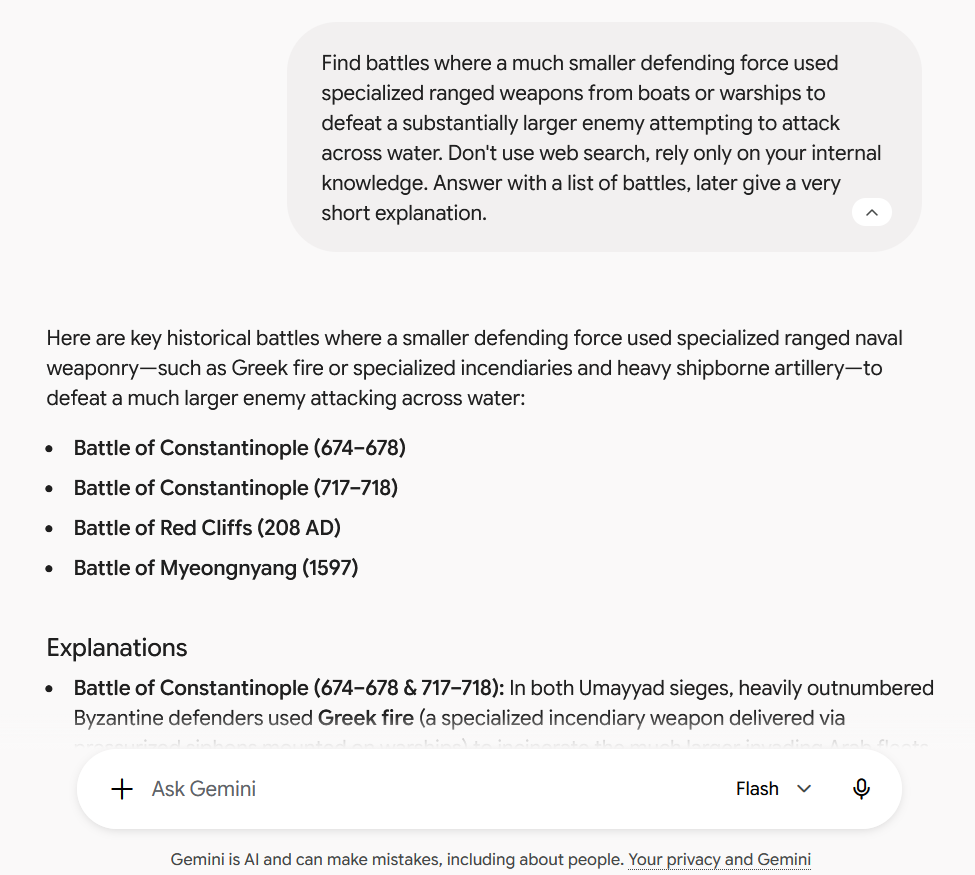
\includegraphics[width=0.75\textwidth]{figures/gemini_initial_response.png}
    \caption{Initial Gemini response to a complex historical battle query.}
    \label{fig:gemini_initial_response}
\end{figure}

\begin{figure}[!htbp]
    \centering
    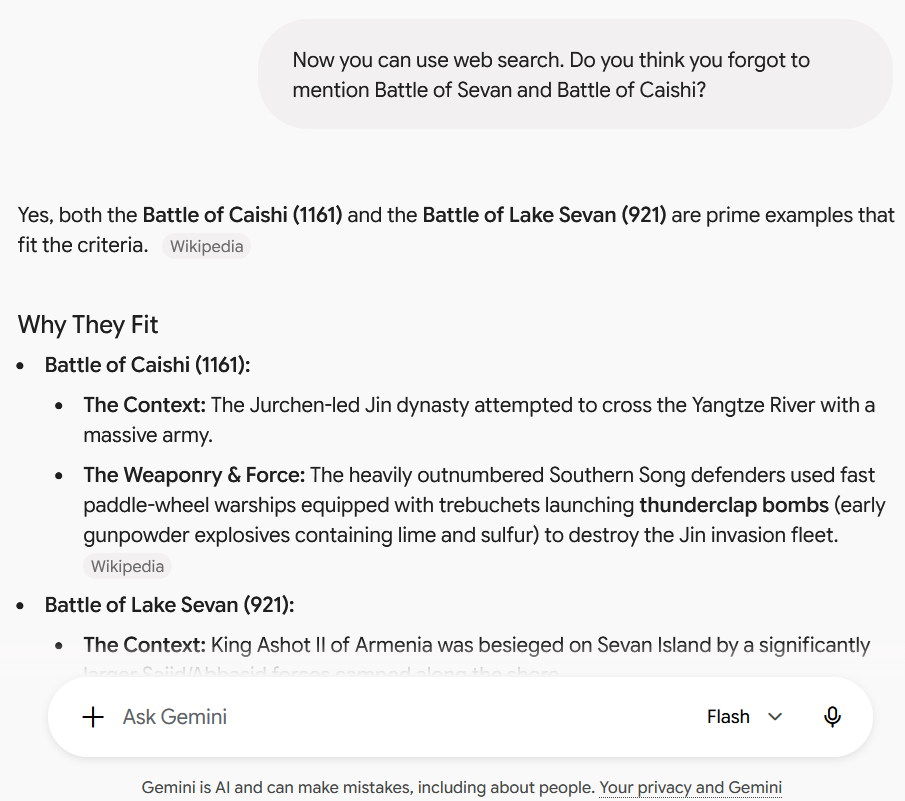
\includegraphics[width=0.75\textwidth]{figures/gemini_followup_response.png}
    \caption{Gemini response to a follow-up query, acknowledging the omission of the Battles of Caishi and Lake Sevan from the initial answer.}
    \label{fig:gemini_followup_response}
\end{figure}

\begin{figure}[!htbp]
    \centering
    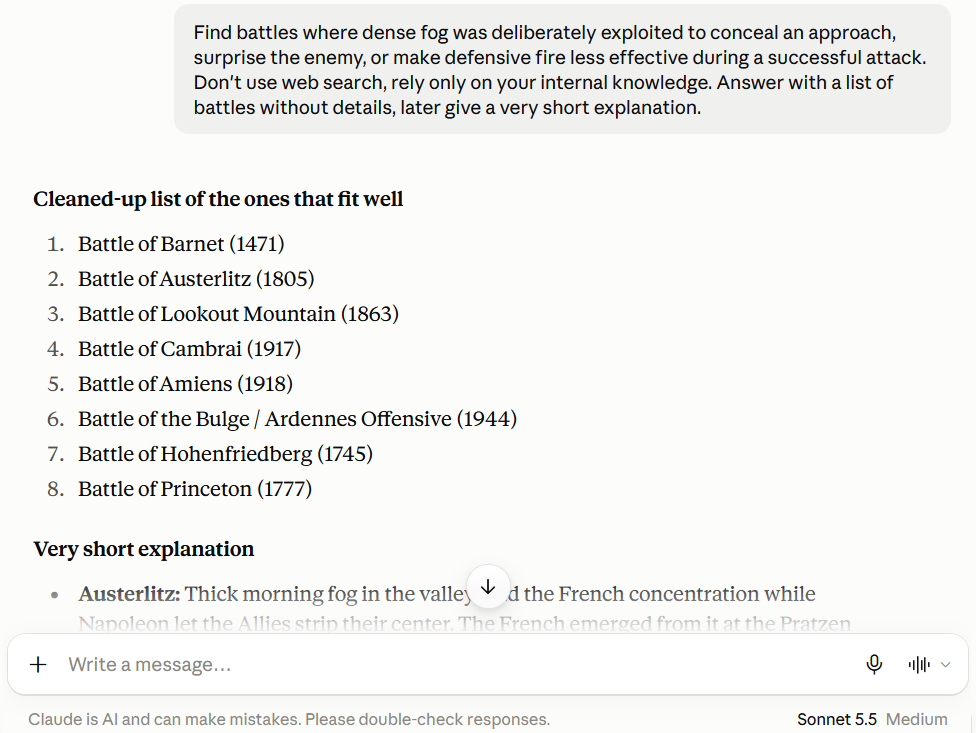
\includegraphics[width=0.85\textwidth]{figures/claude_initial_response.png}
    \caption{Initial Claude response to a complex historical battle query.}
    \label{fig:claude_initial_response}
\end{figure}

\begin{figure}[!htbp]
    \centering
    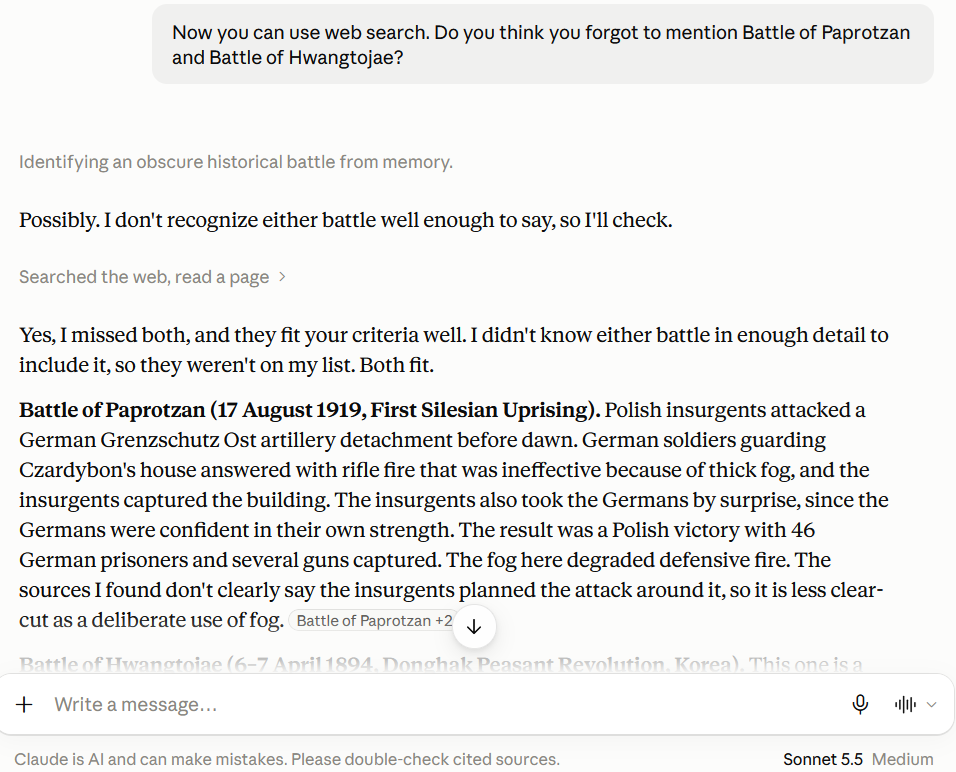
\includegraphics[width=0.85\textwidth]{figures/claude_followup_response.png}
    \caption{Claude response to a follow-up query, acknowledging the omission of the Battles of Paprotzan and Hwangtojae after using web search.}
    \label{fig:claude_followup_response}
\end{figure}

\begin{figure}[!htbp]
    \centering
    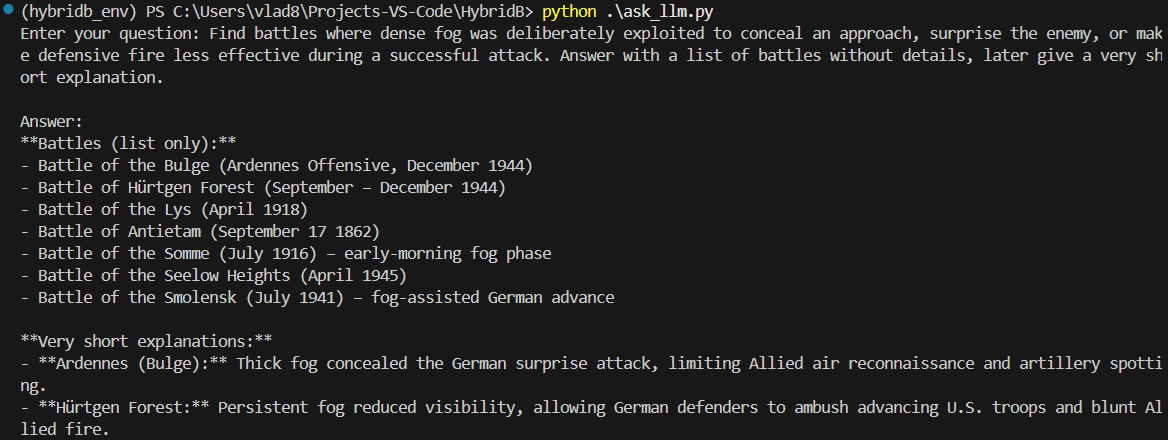
\includegraphics[width=0.99\textwidth]{figures/gpt_oss_fog_query.png}
    \caption{GPT-OSS-120B response to a historical battle query involving the tactical use of fog, generated using the model's internal knowledge without external retrieval.}
    \label{fig:gpt_oss_fog_query}
\end{figure}

\begin{lstlisting}[
    style=sqlstyle,
    caption={SQL-style representation of a historical battle query involving specialized naval weapons and numerical superiority.},
    label={lst:naval_query}
]
SELECT battle
FROM battles
WHERE defender_strength / attacker_strength < 0.5
  AND defender_weapon_type = 'specialized ranged weapon'
  AND defender_platform IN ('boat', 'warship')
  AND attacker_terrain = 'water crossing'
  AND winner = 'defender';
\end{lstlisting}

\begin{minipage}{\textwidth}
\begin{lstlisting}[
    style=sqlstyle,
    caption={SQL-style representation of a historical battle query involving the deliberate tactical exploitation of fog.},
    label={lst:fog_query}
]
SELECT battle
FROM battles
WHERE weather_condition = 'dense fog'
  AND fog_exploitation = 'deliberate'
  AND tactical_effect IN (
      'conceal approach',
      'surprise enemy',
      'reduce defensive fire effectiveness'
  )
  AND attack_outcome = 'successful';
\end{lstlisting}
\end{minipage}

The aim of this thesis is to investigate whether structured battle representations can improve the factual accuracy and overall quality of LLM-generated answers in the domain of historical battles. For this purpose, we first design a structured battle representation schema and construct a local knowledge base containing structured battle representations. We then analyze different retrieval strategies and compare different context-augmented model configurations.

\section{Problem Statement}
\label{sec:problem-statement}
Recent studies on event-centric knowledge representation motivate structured representations for narrative-rich knowledge \citep{guan2023eventkg}. Research on narrative understanding further highlights the importance of capturing information beyond isolated facts, including temporal and event structure \citep{hamilton2026narrabench}. However, it remains unclear whether rich structured representations can substantially improve the accuracy of answers, particularly in the domain of historical battles. Our work investigates whether an LLM provided with additional structured context can produce more accurate and better-grounded answers than the same model relying only on its internal knowledge or on raw textual battle passages. By design, when we evaluate the augmented models, we instruct them not to use their internal knowledge. This makes it easier to determine whether a correct answer is supported by the provided context rather than by the model’s parametric memory. By explicitly requiring the model to rely only on the supplied battle records, the experiment evaluates whether the structured knowledge base contains sufficient information to answer the questions and whether the model can successfully extract and reason over that information. This also enables a more controlled comparison with raw-text augmentation, where the model receives information from the same underlying sources, but in the form of raw-text Wikipedia passages.

This problem becomes more challenging at scale. In this work, we consider 11,561 battle instances identified through Wikidata \citep{vrandecic2014wikidata}, so relevant battle representations must first be retrieved from a large candidate knowledge base before they can be provided to the LLM. This makes retrieval quality another central challenge for this thesis. Prior work on dense retrieval has highlighted the importance of retrieval quality for downstream question-answering performance in open-domain QA \citep{karpukhin2020dpr}. This study evaluates both top-$k$ retrieval accuracy and end-to-end QA performance, illustrating the connection between the retrieved context and the final answer. Following a similar evaluation approach, we investigate three different retrieval strategies and compare their ability to identify relevant battles from all 11,561 instances. This allows us to determine which retrieval strategy is the most effective for our task.
\section{Research Questions}
\label{sec:research-questions}
In this thesis, we consider three main research questions, referred to as RQ1–RQ3.

RQ1. How can historical battles be represented through a structured schema that captures factual, military, temporal, spatial, participant-related, outcome-related, and narrative information?

RQ2. How do lexical, dense, and hybrid retrieval methods perform when retrieving relevant battle representations from a large structured battle knowledge base?

RQ3. How does the use of structured battle representations as external evidence affect LLM-based question-answering quality compared with direct LLM querying and raw-text augmentation?
\section{Our Approach}
\label{sec:our-approach}
To address these research questions, we first define a domain-specific representation schema for historical battles. At the conceptual level, each battle is represented as an event containing quantitative and factual properties, such as date, location, participants’ strength, and losses, as well as military-domain attributes and narrative information, including event order, turning points, narrative patterns, and consequences. Based on this conceptual representation, we design a JSON schema that organizes this information into predefined fields.

The next step is to populate this representation at scale. We identify historical battle instances through Wikidata and retrieve the raw text of their corresponding Wikipedia articles using the Wikipedia API. We then use an LLM to process the collected articles and populate the predefined JSON schema for each battle instance. Following this process, we obtain a structured knowledge base of historical battle representations.

As the next important step, we investigate three retrieval strategies for selecting relevant battles from the knowledge base. These strategies include lexical, dense, and hybrid retrieval. The retrieved battle representations are then provided to the LLM as external context during the question-answering experiments. For the evaluation, we prepare several query types, including temporal, spatial, participant-based, military, tactical, narrative, outcome-related, and similarity-based queries.

In the final step, we conduct experiments with three different LLM question-answering setups. We compare a baseline LLM that relies only on its internal knowledge with a JSON-augmented LLM that receives structured battle representations as additional context and a raw-text-augmented LLM that uses unstructured battle descriptions from the corresponding Wikipedia articles as context. Our experiments cover both retrieval and answer generation. We first compare the retrieval strategies to determine which one is most effective for selecting relevant battle representations. The selected retrieval strategy is then used in the downstream question-answering experiments. Then, the three experimental setups are evaluated using predefined metrics.
\section{Contributions}
\label{sec:contributions}
The main contributions of this thesis are the following:

\begin{enumerate}
    \item We design a domain-specific structured representation schema for historical battles that combines factual and military information with narrative aspects such as ordered events, turning points, participant tactics, action sequences, and narrative patterns.

    \item We construct a large-scale structured knowledge base containing 11,561 historical battle representations. The knowledge base is built from Wikidata and English Wikipedia articles and populated automatically using our implemented LLM-based extraction pipeline. We additionally introduce a verification and regeneration stage to improve the consistency and completeness of the generated battle representations.

    \item We implement and compare three retrieval strategies for structured battle representations: lexical retrieval with BM25, dense retrieval using embeddings, and hybrid retrieval based on Reciprocal Rank Fusion. We evaluate these methods across multiple query types.

    \item We construct an evaluation benchmark of 102 historical battle queries with predefined gold battle sets, query types, context rarity, and closed-set negative examples. This benchmark is used to evaluate both retrieval and answer-generation performance.

    \item We evaluate the effect of structured battle representations on LLM-based question answering through both the Oracle-context experiment, where the LLM is provided with a predefined set of candidate battles to choose from, and the end-to-end RAG experiment. We compare a baseline LLM with raw-text-augmented and JSON-augmented configurations and analyze performance across common and rare battles, different query types, and different retrieval depths.
\end{enumerate}
Our experiments show that structured JSON context is particularly beneficial for rare-battle queries and mainly improves the model’s ability to recover relevant battles. At the same time, the results demonstrate that final end-to-end performance remains strongly dependent on retrieval quality.

\chapter{Related work}
In this chapter, we review several previous works that are relevant to our thesis. We discuss papers on narrative and event-centered representations, schema-guided information extraction, retrieval methods, and retrieval approaches for battle-specific information. The main goal of this chapter is to provide the conceptual background for our work, covering the main aspects of our implementation, such as representing battles as structured events, extracting information from web articles, retrieving relevant battles, and evaluating the final question-answering pipeline.

\section{Narrative Representations}
In this thesis, we treat historical battles as event structures. They contain both factual information, such as date, location, participants, and outcome, and event-centered narratives that involve the temporal development of actions, each side’s objectives, turning points, and consequences. Several previous works support the idea of representing a battle instance as a structured event containing these types of information. 

\citet{chambers2010narrativeschemas} motivates the use of structured event knowledge for document-level understanding tasks such as information extraction, coreference, summarization, and inference. Their work argues that modeling event participants and temporal relations, rather than treating events as isolated facts, can improve narrative understanding. 

Another work on Event Knowledge Graphs (EKGs) \citep{guan2023eventkg} discusses event-centered knowledge representations that capture different aspects of events, such as participants, temporal development, and relations between events. 

\citet{hamilton2026narrabench} also supports the use of broader narrative structures for narrative understanding, particularly temporal aspects such as the order and duration of events.

Overall, these ideas motivate the design of our battle representation schema. In our case, we do not construct a knowledge graph; instead, we follow similar event-centered principles and organize the extracted information within a predefined JSON representation schema. Our battle representations therefore include both quantitative characteristics and narrative-rich information, making them suitable for simple factual questions as well as more complex analyses of narratives, tactics, and outcomes.
\section{Schema-guided event extraction}
After we define the representation schema, the next challenge is to extract the required information from raw text and map it into the predefined JSON schema. We use Wikipedia articles as the source of unstructured information about historical battles. The process of extracting historical battle information is related to event extraction \citep{lai2022eventextraction} and schema-guided knowledge extraction \citep{luo2025oneke}, where information about events, participants, and relations is extracted from raw documents and organized according to a predefined structure. In this subsection, we describe three relevant works that provide useful ideas for our approach.

We define a historical battle instance as an event, so we plan to extract it in the same way as other event structures. \citet{lai2022eventextraction} describes event extraction as an information extraction task that identifies events in text and organizes them into predefined structures or classes. The survey also suggests describing event information through elements such as participants, roles, time, and location.

Recent work on schema-guided LLM extraction \citep{luo2025oneke} presents an approach where LLMs are used to extract structured knowledge from raw text. The work suggests that knowledge extraction can benefit from well-defined schema design, validation, and correction. Such schemas can be represented in JSON format.

Another work on schema-aware event extraction argues that event extraction can support downstream tasks such as question answering and information retrieval \citep{liang2025asee}. The work also discusses the problem of “schema hallucination”, where LLMs may invent non-existent event types during extraction if they are not sufficiently constrained \citep{liang2025asee}. 

Following these ideas, we plan to use Wikipedia articles on historical battles to extract key information and populate our predefined JSON schema. As described in the schema-guided extraction approach, we define a JSON schema and then use an LLM to populate it with information extracted from raw Wikipedia articles. The use of a fixed JSON schema with predefined fields is also important for guiding the LLM extraction process and preventing the model from generating arbitrary structures.
\section{Retrieval Methods and RAG}
After we constructed a knowledge base with structured battle representations, the next goal is to build a retrieval pipeline that looks for relevant battles depending on a given query. At this stage, retrieval quality becomes a central challenge. In our work, we investigate different retrieval approaches, including lexical, dense, and hybrid methods, and test them over 11,561 battle instances. In this subsection, we discuss several relevant papers that motivate different retrieval methods used in our experiments.

To choose the most effective retrieval approach, we investigated a work that directly compares traditional sparse retrieval methods such as TF-IDF and BM25 with dense retrieval methods. BM25 is a probabilistic ranking function that scores documents based on term frequency saturation, document length normalization, and inverse document frequency (IDF) to estimate their relevance to a given query \citep{robertson2009bm25}. Conversely, dense retrieval performs information retrieval by mapping questions and passages into a low-dimensional latent semantic space rather than relying on sparse keyword matching methods such as TF-IDF or BM25 \citep{karpukhin2020dpr}.

The HybridRAG paper \citep{sarmah2024hybridrag} paper discusses some limitations of classical vector-based RAG and structured graph retrieval. It mentions that vector-based RAG may retrieve semantically similar chunks but can struggle to preserve structured context. Meanwhile, structured graph retrieval can capture relations but may still struggle with broader semantic information. The authors introduce an approach that combines both methods into a hybrid RAG system to improve question answering over complex data. 

In our work, we also investigate how lexical and dense retrieval methods perform and evaluate a combined approach called hybrid retrieval. Unlike HybridRAG, we do not work with knowledge graphs. Instead, we work with structured battle representations and combine lexical retrieval with dense retrieval within the RAG pipeline. This allows us to benefit from both lexical matching and semantic similarity and potentially improve the quality of battle retrieval.
\section{Battle-specific Retrieval}
As discussed in earlier parts, battle-specific questions require both factual data and information about ordered actions, temporal development, narratives, tactics, and outcomes. Thus, when we consider retrieval in the historical battles domain, we should focus on the natural structure of a battle. In this subsection, we discuss several works related to event-aware retrieval and battle-specific similarity modeling.

\citet{yang2025eventrag} discuss the limitations of conventional RAG approaches for narrative-rich information. They argue that traditional RAG systems usually process text at the level of documents, passages, or sentences and may therefore fail to capture the underlying event structures that describe real-world narratives. The authors therefore propose organizing the retrieved knowledge into an event-centric representation that captures relations between events and their temporal development. This idea is related to our work, where we also work with narrative-rich historical battles and therefore need the LLM to consider not only factual, but also narrative information.

Another recent work on the historical battles domain showed that there are some limitations in describing battles using only quantitative statistics \citep{coulson2023actionclusters}. The authors noticed that simple statistics may miss several aspects of battles, such as relationships between actions and collaboration, so higher-level descriptors are needed to capture such aspects. In their approach, the model learns latent representations of actions and units within battles, which can reveal more insights into similarities between tactical behavior and the strategies of participants. This directly supports our idea that we need to describe a battle with more than just simple factual metadata.

The RAGAS paper \citep{es2024ragas} introduces several ideas that are relevant to the evaluation of our RAG pipeline. The paper presents a framework for evaluating RAG pipelines across three quality metrics: faithfulness, answer relevance, and context relevance. These metrics show how well the generated answer is supported by the given context, whether it addresses the initial question, and how relevant the retrieved context is. This is useful for our work because it provides more insight into how well the LLM uses the provided context and whether the context itself is relevant and not too noisy.
\chapter{Methodology}
This chapter describes the methodology used to construct and evaluate our historical battle question-answering pipeline, named HybridB. First, we explain how the battle corpus is collected and transformed into structured JSON representations, including the LLM-based population, verification, and regeneration stages. Second, we describe the three retrieval methods used to identify relevant battle instances: lexical, dense, and hybrid retrieval. Finally, we present the answer-generation setup used to compare baseline, JSON-augmented, and raw-text-augmented LLM configurations. The project can be accessed through the following GitHub repository: \url{https://github.com/Sandora1933/HybridB}
\section{Data Sources and Knowledge Base Construction}
First, we need a centralized source of historical battles. Figure~\ref{fig:battle_data_collection} shows the complete process of gathering the initial data from the source and constructing our local knowledge base of raw-text articles.

\begin{figure}[!htbp]
    \centering
    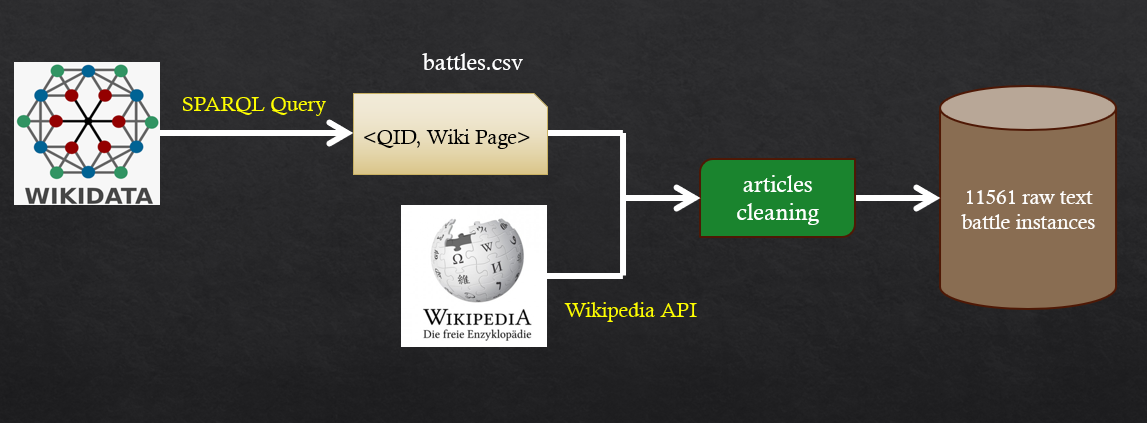
\includegraphics[width=\textwidth]{figures/battle_data_collection.png}
    \caption{Historical battle data collection pipeline.}
    \label{fig:battle_data_collection}
\end{figure}

Wikidata is a central storage system for structured data used across sister projects such as Wikipedia. The Wikidata repository consists mainly of items, where each item has a label, a description, and optionally a number of aliases. Items are uniquely identified by a \texttt{Q} followed by a number, for example Battle of Leipzig (\texttt{Q151005}). Statements describe characteristics of an item and consist of a property and a value. Properties in Wikidata are identified by a \texttt{P} followed by a number, such as \texttt{P31} for \textit{instance of} \citep{wikidata2026introduction}. Wikidata provides an efficient way to retrieve historical battle instances using the SPARQL query language. SPARQL is the W3C-standard query language for RDF graph data, which we mainly use to retrieve Wikidata entities and their corresponding historical battle pages on Wikipedia \citep{harris2013sparql}. Listing~\ref{lst:wikidata_sparql} shows the SPARQL query used to retrieve all Wikidata battle instances and filter them to include only entities that have a corresponding English Wikipedia page. The predicate wdt:P31 represents the property \textit{instance of}, while the object wd:\texttt{Q178561} represents the Wikidata item \textit{battle}. In natural language, the query means: \textit{Retrieve all distinct Wikidata entities that are classified as instances of a battle} (\texttt{Q178561}) \textit{and have a corresponding article in the English-language Wikipedia, returning both the Wikidata entity and its Wikipedia article URL.}

\begin{minipage}{\textwidth}
\begin{lstlisting}[
    style=sqlstyle,
    caption={SPARQL query for retrieving historical battle entities from Wikidata and their corresponding English Wikipedia articles.},
    label={lst:wikidata_sparql}
]
SELECT DISTINCT ?item ?wikipediaArticle WHERE {
    ?item wdt:P31 wd:Q178561.

    ?wikipediaArticle schema:about ?item;
        schema:isPartOf <https://en.wikipedia.org/>.
}
\end{lstlisting}
\end{minipage}

After executing the SPARQL query, the results were processed to create a clean list of battle instances. For each retrieved entity, the QID was extracted from the entity URI and paired with the corresponding English Wikipedia article URL. Duplicate entities were removed using the QID as the unique identifier, and the remaining records were sorted by QID. The resulting dataset was then stored as a CSV file containing one row for each battle instance together with the corresponding English Wikipedia page, as illustrated in Table 3.1.
\begin{table}[htbp]
    \centering
    \caption{Example entries from the collected battle dataset}
    \label{tab:battle_dataset}
    \begin{tabular}{c c l}
        \toprule
        \textbf{\#} & \textbf{qid} & \textbf{wikipedia\_url} \\
        \midrule
        1 & Q330 & \url{https://en.wikipedia.org/wiki/Battle_of_Marignano} \\
        2 & Q1392 & \url{https://en.wikipedia.org/wiki/Battle_of_Nieuwpoort} \\
        \vdots & \vdots & \vdots \\
        11561 & Q140628890 & \url{https://en.wikipedia.org/wiki/Battle_of_Bizye_(1256)} \\
        \bottomrule
    \end{tabular}
\end{table}

Following this step, for each battle instance from the resulting list, we programmatically retrieve the associated Wikipedia article in raw text format using the wikipediaapi Python library \citep{wikipediaapi}. The extracted article text contains the page summary and article sections. Non-content sections such as references, external links, citations, and bibliographies are not included. After cleaning, the text of each article is stored locally as a UTF-8 text file named after its Wikidata QID. At this stage, we obtain the raw textual knowledge base containing 11,561 battle instances collected using Wikidata and Wikipedia.
\section{Battle Representation Schema}
Following the ideas discussed in Chapter 2.1, we decided to design a structured battle representation schema that can later be populated with real information from our battle sources. In general, our representation schema is a JSON structure containing 10 top-level categories and 85 individual fields (leaf fields), covering basic factual information about the battle as well as higher-level aspects such as military facets, narratives, narrative patterns, outcomes, and summaries. Figure~\ref{fig:battle_schema} shows the overall structure of our representation schema.

\begin{figure}[!htbp]
    \centering
    \begin{subfigure}[t]{0.47\textwidth}
        \centering
        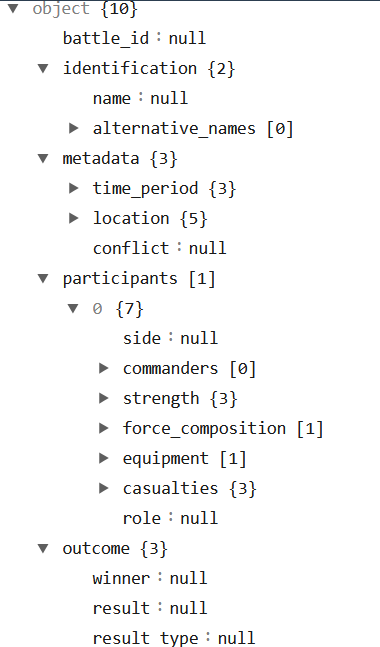
\includegraphics[width=\linewidth]{figures/battle_schema_a.png}
        \caption{Identification, metadata, participants, and outcome.}
        \label{fig:battle_schema_a}
    \end{subfigure}
    \hfill
    \begin{subfigure}[t]{0.47\textwidth}
        \centering
        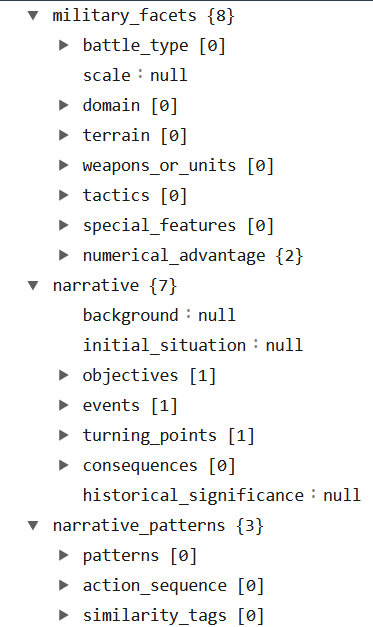
\includegraphics[width=\linewidth]{figures/battle_schema_b.png}
        \caption{Military facets, narrative, and narrative patterns.}
        \label{fig:battle_schema_b}
    \end{subfigure}

    \caption{Overview of the structured representation schema for historical battles, illustrating its main information categories and nested fields.}
    \label{fig:battle_schema}
\end{figure}

When we design a battle representation, we consider relevant aspects that can later help the LLM with reasoning. We start with \texttt{battle\_id} and identification fields to be able to distinguish between battles during debugging. Apart from battle names, we also include alternative names for cases where a battle is known under different names. For instance, in Wikidata, the Battle of Leipzig (\texttt{Q151005}) is also known as the Battle of the Nations. 

Next, we define metadata fields such as \texttt{time\_period}, \texttt{location}, \texttt{conflict}, and \texttt{country\_modern}. The \texttt{time\_period} includes a start date and an end date in ISO format, for example \texttt{1515-09-13}, and additionally a human-readable date label such as \textit{13 September 1515}. \texttt{country\_modern} is a field that describes the modern country located on the territory where the battle occurred. It can be useful for queries such as \textit{Describe battles involving a double envelopment that occurred in the 16th century on the territory of modern Germany.} To be precise, \texttt{country\_modern} contains several edge cases where the modern country is difficult to define, for example when a battle occurred across the territory of several modern countries, as in the Battle of the Bulge (1944–1945), or when the modern country is not universally recognized, as in the case of Kosovo for the Battle of Kosovo (1389).

The next aspect is participants. Here, information about sides, commanders, strength, force composition, and other related details is captured. Each side includes a list of commanders who participated in the battle, while the \texttt{strength} field contains the number of troops, including different troop types. For instance, the total strength can be 3,100 with the label \textit{1,100 knights, 2,000 infantry}. If a side is a coalition of several nations, we explicitly define the strength of each participant in the note. For example, for the Coalition side in the Battle of Leipzig: \textit{Estimates of 380,000 troops with 1,500 guns; breakdown: Russians 145,000–150,000, Austrians 115,000, Prussians 75,000–90,000, Swedes 19,000–30,000.} Then, for each contingent involved on each side, we describe the force composition in detail, specifying its size, unit types, equipment, casualties, and role in the battle. This information is relevant for queries such as \textit{Which battles involved a coalition of multiple nations fighting against a numerically superior enemy?}, where the model needs information about the coalition sides and the sizes of their forces. Besides, equipment and unit types can be very useful when we want to ask the model which side had more tanks or artillery but did not gain a terrain advantage and still lost the battle.

To be able to reason over battle outcomes and obtain more concrete insights into the results, we include an additional \texttt{outcome} field that specifies the \texttt{winner}, \texttt{result}, and \texttt{result\_type}. The \texttt{result} field describes the nature of the outcome. It can represent, for example, a \textit{decisive victory}, a \textit{successful defense}, a \textit{successful withdrawal}, or an inconclusive result when it is difficult to summarize the outcome clearly. The \texttt{result} is expressed from the perspective of the side identified as the \texttt{winner}, when applicable. The \texttt{result\_type} field describes the significance of the outcome. For instance, \textit{tactical} means an immediate battlefield success, \textit{operational} refers to a success affecting a campaign or series of battles, while \textit{strategic} describes a broader success affecting overall war objectives. Naturally, such classifications can be subjective and depend on interpretation. These questions, together with possible future improvements, are discussed in Chapter 6, Discussion.

Next, we describe the military facets, which capture the key military characteristics of a battle. They include fields such as \texttt{battle\_type}, \texttt{scale}, \texttt{domain}, \texttt{terrain}, \texttt{weapons\_or\_units}, \texttt{tactics}, and \texttt{special\_features}. Most of these fields are represented as lists and can therefore contain multiple descriptions, while scale is represented as a single value. The \texttt{battle\_type} field describes the general type of engagement, for example a land battle. The \texttt{scale} field indicates the overall size of the battle. The \texttt{domain} field specifies whether the battle took place on land, at sea, in the air, or across multiple domains. The \texttt{terrain} field describes the main environmental conditions that may affect the battle, such as urban, riverine, mountainous, or village terrain. \texttt{weapons\_or\_units} captures important types of troops and military equipment involved in the engagement, for example infantry, cavalry, artillery, or rockets. The \texttt{tactics} field describes important tactical approaches used during the battle, such as encirclement, defense of bridges, or urban street fighting. Finally, \texttt{special\_features} is used to store particularly distinctive characteristics of a battle, for example the use of Congreve rockets or a Grand Battery of 150 guns in the case of the Battle of Leipzig. These fields are important for queries that require reasoning over the military characteristics of battles, for example comparing battles with similar terrain, identifying battles where particular weapons or tactical approaches were used, or finding battles with unusual military features. One example of such a query is the following: \textit{Which land battles involved fighting in urban areas and near rivers, where commanders employed encirclement tactics and concentrated artillery batteries?}

To improve narrative reasoning, we define a narrative aspect of a battle. It shows how the battle developed over time and describes individual events in chronological order, as well as how they are connected to the broader course of the engagement. The \texttt{narrative} top-level field includes \texttt{background}, \texttt{initial\_situation}, \texttt{objectives} of each side, \texttt{events}, \texttt{turning points}, \texttt{consequences}, and \texttt{historical\_significance}. Each event includes its order number, phase, event type, actors, targets, description, outcome, and optionally its causal role and confidence. This makes our representation able to capture important insights about the order of events and involved actors, and to assign a specific role, target, and outcome to each event. This may help to understand whether a specific side had an advantage over the whole duration of the battle or only at a specific moment. We can also gain more insight into how the engagement developed over time and how the winner ultimately achieved victory. The \texttt{turning\_points} field helps to define important moments that significantly changed the course of the battle, for example the Coalition encirclement of the French army during the Battle of Leipzig. We also define a \texttt{consequences} field that captures the main political and military outcomes after the battle. \texttt{historical\_significance} additionally provides information about the broader importance of the battle. Good examples of queries that may require this narrative aspect are queries asking to find battles involving an initially successful defense followed by encirclement and retreat, or battles where a tactical turning point later caused a broader strategic defeat.

Apart from the narrative aspect, we additionally define a \texttt{narrative\_patterns} field that captures higher-level narrative structures. It contains battle \texttt{patterns}, an \texttt{action\_sequence}, and \texttt{similarity\_tags}. The \texttt{patterns} field describes tactical and narrative characteristics of the battle, for example encirclement, urban street fighting, or the use of massed artillery. The \texttt{action\_sequence} field describes the main stages of the battle in a simplified chronological form. We additionally define a \texttt{similarity\_tags} field to explicitly mark comparable characteristics that might be useful when trying to find similar battles, for instance large-scale coalition battles, defeats of Napoleon, or battles involving multi-nation forces.

In the \texttt{retrieval\_texts} field, compact textual summaries are described. They are generated from the structured battle representation and are designed to support retrieval. Specifically, it contains a \texttt{tactical\_summary}, \texttt{narrative\_summary}, and \texttt{action\_sequence\_summary} that partially duplicate values defined in the narrative field. The initial motivation for introducing the \texttt{retrieval\_texts} field was to provide condensed, semantically informative descriptions of battles that could improve dense retrieval without requiring embedding models to process the entire JSON representation. However, as described later in the Retrieval chapter, our implemented retrieval approach serializes and embeds complete JSON documents without separately extracting or prioritizing these summaries. Therefore, although the generated summaries contribute to the input representation, their independent impact on retrieval and answer generation quality remains unknown.

Finally, we added \texttt{extraction\_metadata} to our representation schema. It stores information about the extraction process and possible uncertainty in the generated battle representation. It contains fields such as \texttt{wikidata\_id}, \texttt{overall\_confidence}, and \texttt{uncertainty\_notes}. The \texttt{field\_confidence} field indicates how reliable the extracted information is and is defined automatically by the filler LLM for most top-level aspects. In addition, \texttt{uncertainty\_notes} is used to mark conflicting or uncertain information from the source. It is especially useful for avoiding the need to force a single value, for instance for troop strength or the number of casualties. It can contain information such as \textit{French total strength estimates range from 198,000 to 225,000.}

The schema fields, their descriptions, and data types are also provided in Table~\ref{tab:battle_schema}.
\begin{table}[!htbp]
\centering
\caption{Overview of the structured battle representation schema}
\label{tab:battle_schema}

\footnotesize
\renewcommand{\arraystretch}{1.4}
\setlength{\tabcolsep}{4pt}

\begin{tabularx}{\textwidth}{
    >{\RaggedRight\arraybackslash}p{0.13\textwidth}
    >{\RaggedRight\arraybackslash}X
    >{\RaggedRight\arraybackslash}p{0.32\textwidth}
    >{\RaggedRight\arraybackslash}p{0.09\textwidth}
}
\toprule
\textbf{Battle aspect} &
\textbf{Schema fields} &
\textbf{Description} &
\textbf{Datatype} \\
\midrule

\textbf{Battle ID} &
\texttt{battle\_id} &
Unique identifier of the battle instance, typically corresponding
to its Wikidata QID. &
String / null \\
\midrule

\textbf{Identification} &
\texttt{identification.name},
\texttt{identification.alternative\_names} &
Stores the primary battle name and possible alternative names. &
Object \\
\midrule

\textbf{Metadata} &
\texttt{time\_period},
\texttt{location},
\texttt{conflict};
e.g. \texttt{start\_date},
\texttt{end\_date},
\texttt{country\_modern} &
Contains basic factual metadata about when and where the battle
occurred and the wider conflict it belongs to. &
Object \\
\midrule

\textbf{Participants} &
\texttt{side},
\texttt{commanders},
\texttt{strength},
\texttt{force\_composition},
\texttt{equipment},
\texttt{casualties},
\texttt{role} &
Represents the participating sides and their commanders,
force size, composition, equipment, casualties, and role
in the battle. &
\texttt{Array\textless Object\textgreater} \\
\midrule

\textbf{Outcome} &
\texttt{winner},
\texttt{result},
\texttt{result\_type} &
Describes the final result of the battle, including the
winning side and the type of victory or outcome. &
Object \\
\midrule

\textbf{Military facets} &
\texttt{battle\_type},
\texttt{scale},
\texttt{domain},
\texttt{terrain},
\texttt{weapons\_or\_units},
\texttt{tactics},
\texttt{special\_features},
\texttt{numerical\_advantage} &
Captures important military characteristics of the battle
such as terrain, tactics, force types, weapons, and
numerical advantage. &
Object \\
\midrule

\textbf{Narrative} &
\texttt{background},
\texttt{initial\_situation},
\texttt{objectives},
\texttt{events},
\texttt{turning\_points},
\texttt{consequences},
\texttt{historical\_significance} &
Represents how the battle developed, including its
background, objectives, sequence of events, key turning
points, consequences, and historical importance. &
Object \\
\midrule

\textbf{Narrative patterns} &
\texttt{patterns},
\texttt{action\_sequence},
\texttt{similarity\_tags} &
Stores higher-level recurring patterns and abstract action
sequences that can support comparison between battles. &
Object \\
\midrule

\textbf{Retrieval texts} &
\texttt{short\_summary},
\texttt{tactical\_summary},
\texttt{narrative\_summary},
\texttt{action\_sequence\_summary},
\texttt{similarity\_query\_text} &
Contains compact textual representations of the battle
designed to support different retrieval and similarity tasks. &
Object \\
\midrule

\textbf{Extraction metadata} &
\texttt{wikidata\_id},
\texttt{overall\_confidence},
\texttt{field\_confidence},
\texttt{uncertainty\_notes} &
Stores provenance and confidence information about the
extracted structured representation and notes possible
uncertainty. &
Object \\

\bottomrule
\end{tabularx}
\end{table}
\section{LLM-Based Schema Population}
At this stage, we already have a raw-text knowledge base containing 11,561 historical battle articles and a JSON representation schema covering the relevant aspects of a battle. The next step is to use an LLM to populate the JSON schema for each raw-text battle article. As a result, we obtain a structured knowledge base consisting of 11,561 JSON files, one for each battle instance.

First, we introduce the GPT-OSS-120B model, which was used for the schema population task and also for almost all other LLM-based tasks described later \citep{openai2025gptoss}. The model was accessed through the ScaDS.AI service via its OpenAI-compatible REST API \citep{scadsai2026}. Communication with the service was implemented using the official OpenAI Python client and configured with the ScaDS.AI endpoint. Deterministic decoding was used by setting the temperature to 0.0 and disabling sampling. The maximum generation length was set to 4,000 tokens. The model response was returned as plain text and subsequently processed by the experiment pipeline. We treated responses terminated due to the maximum token limit as generation failures. Likewise, responses with missing content were handled as invalid model outputs.

Next, given the LLM gateway and the local knowledge base of battle articles, we proceed with designing a prompt for the schema-population task. The idea is to ask the model to fill the empty representation schema with values based on the raw-text article. Figure~\ref{fig:battle_extraction_prompt} shows the prompt structure without the 17 additional rules, while all 17 rules included in the prompt are presented below.

\begin{figure}[H]
    \centering
    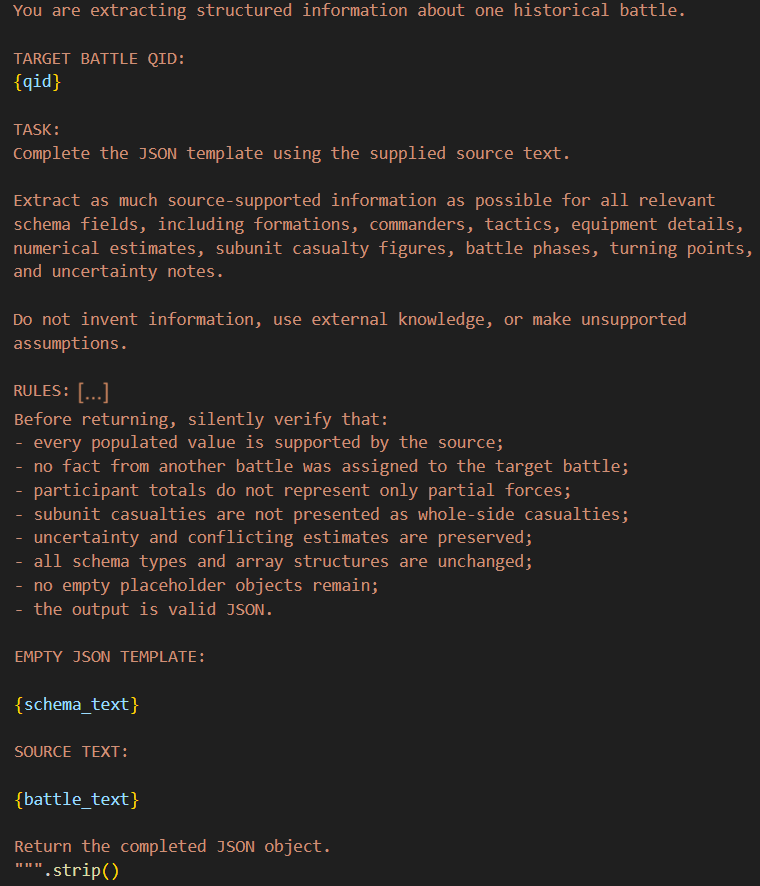
\includegraphics[
        width=0.75\textwidth,
        height=0.45\textheight,
        keepaspectratio
    ]{figures/battle_extraction_prompt.png}
    \caption{Prompt template used to guide GPT-OSS-120B in extracting source information from Wikipedia articles and populating the structured JSON battle representation schema.}
    \label{fig:battle_extraction_prompt}
\end{figure}

\par\medskip
\noindent\textbf{Extraction Rules}
\par\smallskip

\begingroup
\small

\begin{enumerate}[
    leftmargin=1.2cm,
    itemsep=5pt,
    topsep=3pt,
    parsep=0pt,
    label=\textbf{\arabic*.}
]

    \item Use only information supported by the source text. Do not use external or prior knowledge.

    \item Extract information only about the target battle and its directly relevant background, course, outcome, and consequences. Do not assign facts from other battles, unrelated campaign events, or later historical developments to the target battle unless the source explicitly connects them to it.

    \item Preserve the exact JSON structure, field names, nesting, data types, and array item types. Do not add, remove, rename, or restructure fields.

    \item Fill as many fields as the source supports.
    \begin{itemize}[
        leftmargin=1.5em,
        itemsep=2pt,
        topsep=3pt,
        parsep=0pt
    ]
        \item Unsupported scalar fields must be \texttt{null}.
        \item Unsupported arrays must be \texttt{[]}.
        \item Do not return placeholder array objects containing only null or empty values.
        \item Do not fill a field merely to make the JSON appear complete.
    \end{itemize}

    \item Set \texttt{battle\_id} and \texttt{extraction\_metadata.wikidata\_id} to the provided QID.

    \item Preserve uncertainty, ranges, approximations, alternative estimates, and conflicting figures. Do not replace them with unsupported exact values. Use \texttt{label}, \texttt{note}, and \texttt{uncertainty\_notes} where appropriate.

    \item Do not calculate totals unless all components are explicit, complete, unambiguous, and refer to the same side in the target battle. Explain any calculation in the corresponding \texttt{note} field.

    \item A participant strength total must represent the complete supported strength of that side. Do not use the number of one component, such as infantry, as the side's total strength when additional forces are also mentioned.

    \item Include commanders only when the source clearly connects them to command during the target battle. Preserve major allies and supporting contingents that actually participated.

    \item Keep target-battle casualties separate from casualties belonging to other battles, the wider campaign, pursuit, retreat, or later aftermath.

    \item Preserve supported subunit casualty figures, but clearly associate them with the relevant formation or event. Do not present subunit casualties as the total casualties of an entire participant side.

    \item Distinguish equipment used in the battle from captured materiel. Do not treat captured equipment as pre-battle strength.

    \item Concise source-grounded abstraction is allowed for military facets, narrative events, turning points, narrative patterns, similarity tags, and retrieval summaries. Do not invent unsupported facts, motives, causal claims, or specialized terminology.

    \item When the source describes a clear battle sequence, populate chronological narrative events, important turning points, action sequence, and retrieval summaries. Focus on developments important to the overall battle while preserving significant supported details.

    \item Dates:
    \begin{itemize}[
        leftmargin=1.5em,
        itemsep=2pt,
        topsep=3pt,
        parsep=0pt
    ]
        \item Use \texttt{YYYY-MM-DD} for CE \texttt{iso\_date} when day, month, and year are known.
        \item Populate \texttt{duration\_days} only when both boundary dates are precise.
        \item Count duration inclusively.
        \item Do not create non-standard ISO strings for BCE dates.
        \item Record important date inconsistencies in \texttt{uncertainty\_notes}.
    \end{itemize}

    \item Set all confidence fields to \texttt{null}.

    \item Return exactly one valid JSON object. Do not include Markdown, comments, explanations, or text outside the JSON.

\end{enumerate}

In the prompt, the LLM was given a role, a specific task, a set of rules, an output format, and the attached raw-text article together with the empty representation schema.

The 17 rules provided in the prompt are designed to constrain the schema-population process and reduce unsupported outputs. The rules can be divided into several groups based on source grounding, structural consistency, uncertainty handling, and the special interpretation of battle-specific numerical information.

One of the most important rules (Rule 1) forces the model to use only information supported by the source text, without relying on its internal knowledge. This makes the result traceable to the corresponding Wikipedia article. A similar rule (Rule 2) restricts extraction to the target battle, preventing facts from similar battles or the wider campaign from being incorrectly assigned to the target instance.

Among the structural consistency rules, it is worth mentioning Rule 3, which requires the model to preserve the initial JSON structure provided in the \texttt{empty\_schema.json} file. This guarantees that all generated JSON files follow the same pattern. Additionally, Rule 4 instructs the model to fill fields only when they are directly supported by the source and to use \texttt{null} or empty arrays for unsupported information instead of inventing details.

Another group of rules addresses uncertainty and numerical data. Rule 6 instructs the model to preserve value ranges, approximations, alternative estimates, and conflicting figures when no exact value is provided. Rule 7 also states that the model should not calculate totals unless all components are explicit, complete, and unambiguous, which is especially important for troop strength and casualty numbers.

Several rules focus on the narrative representation. In particular, Rules 13 and 14 instruct the model to populate chronological events, turning points, action sequences, and retrieval summaries when they are supported by the source, while still avoiding unsupported claims, causal statements, or invented tactical terminology.

Finally, Rule 17 requires the model to return exactly one valid JSON object without Markdown, comments, or additional explanations.

\begin{figure}[!htbp]
    \centering
    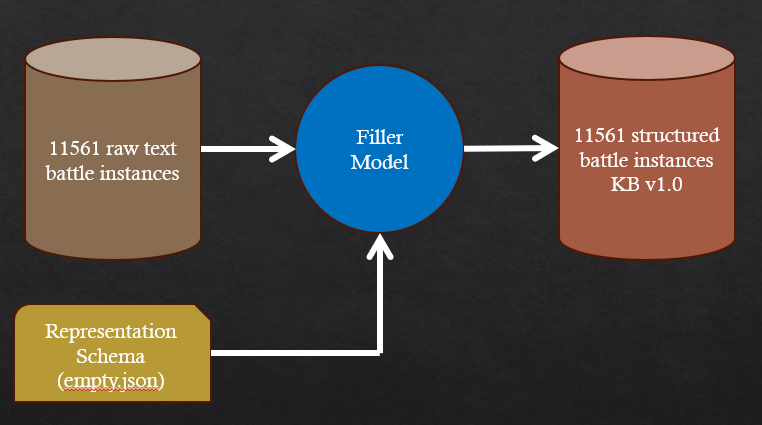
\includegraphics[width=0.95\textwidth]{figures/battle_kb_construction.png}
    \caption{Construction of the structured historical battle knowledge base (KB v1.0).}
    \label{fig:battle_kb_construction}
\end{figure}

As a result, after running the generation pipeline over the entire raw-text knowledge base, we obtain a knowledge base of JSON battle representations, as illustrated in Figure~\ref{fig:battle_kb_construction}. It is worth mentioning that this is only the first version of our JSON knowledge base. In the next section, 3.4, we introduce an additional pipeline with an LLM verifier and a regeneration step, which finally leads to the second version of the JSON knowledge base that is expected to have higher quality.
\section{LLM Verification and Regeneration}
During the analysis of the generated JSON battle representations, we identified several cases where the first version of the knowledge base (KB1) contained incomplete or semantically inconsistent structured information. One example is the Battle of Stalingrad. In KB1, the Soviet force composition contained only a subset of the formations explicitly mentioned in the source article, including the 62nd, 51st, 57th, 24th, and 5th Tank Armies. However, the source also described several additional Soviet formations involved in the later encirclement operation, such as the 28th, 64th, 65th, 66th, 1st Guards, and 21st Armies, as well as several air armies. After verification and regeneration, these missing formations were added in KB2, resulting in a more complete representation of the Soviet forces. The comparison between the corresponding KB1 and KB2 fields is shown in Figure~\ref{fig:kb1_kb2_comparison}.

\begin{figure}[!htbp]
    \centering
    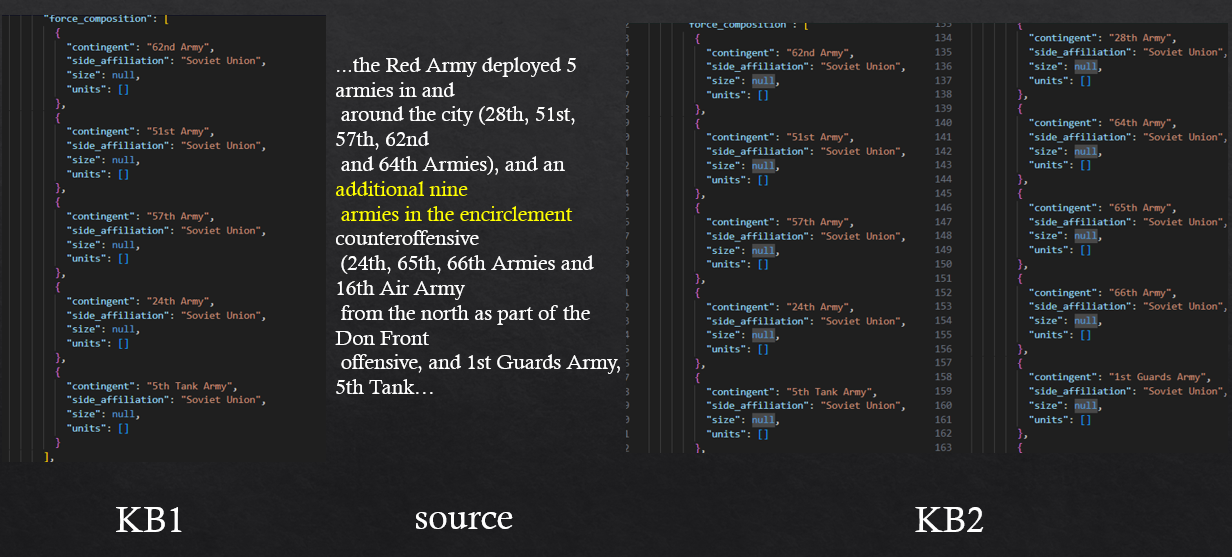
\includegraphics[
        width=\textwidth,
        height=0.75\textheight,
        keepaspectratio
    ]{figures/kb1_kb2_comparison.png}
    \caption{Comparison of the Soviet force composition fields in KB1 and KB2.}
    \label{fig:kb1_kb2_comparison}
\end{figure}

A second example concerns the Battle of Waterloo. In KB1, the role of the Prussian participant was classified as defender. This is inconsistent with the source article, which describes the arriving Prussian forces actively attacking the French flank and advancing toward Plancenoit during the battle. After verification and regeneration, the participant role was corrected to attacker in KB2. Unlike the Stalingrad example, which mainly demonstrates an improvement in completeness, the Waterloo case shows how the verification step can correct the semantic interpretation of a structured field. Figure~\ref{fig:kb1_kb2_participant_roles} illustrates this change between KB1 and KB2.

\begin{figure}[!htbp]
    \centering
    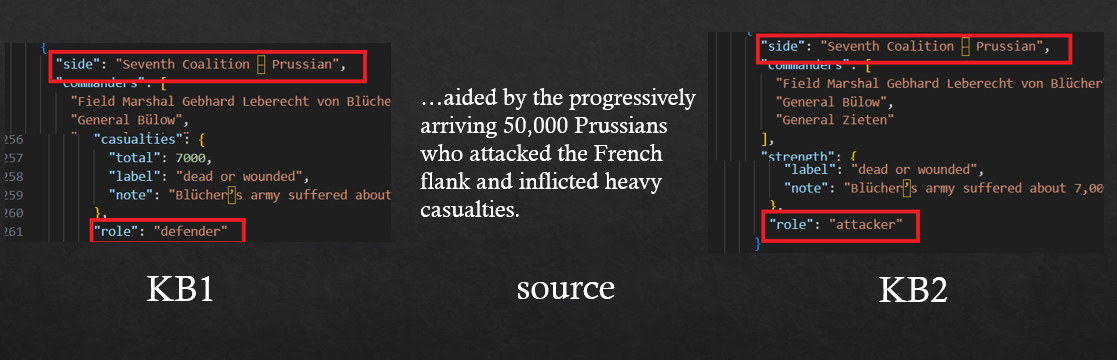
\includegraphics[
        width=\textwidth,
        height=0.75\textheight,
        keepaspectratio
    ]{figures/kb1_kb2_participant_roles.png}
    \caption{Comparison of participant role of Prussian forces in KB1 and KB2.}
    \label{fig:kb1_kb2_participant_roles}
\end{figure}

The design of the verification and regeneration pipeline that led to KB2 is shown in Figure~\ref{fig:kb_verification_refinement}. First, for each battle, the generated KB1 JSON record was paired with its corresponding raw Wikipedia article, which served as the reference source. In the first stage, an LLM verifier compared the structured representation against the source text and identified unsupported information, factual inconsistencies, schema-semantic errors, and important omissions. The verifier returned a structured report containing either a \texttt{PASS} verdict or a \texttt{REVISE} verdict with a list of recommended corrections.

\begin{figure}[!htbp]
    \centering
    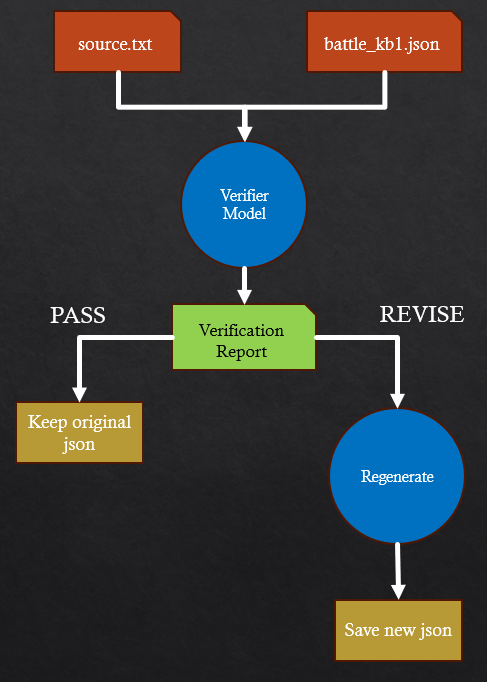
\includegraphics[
        width=\textwidth,
        height=0.40\textheight,
        keepaspectratio
    ]{figures/kb_verification_refinement.png}
    \caption{Knowledge base verification and refinement pipeline.}
    \label{fig:kb_verification_refinement}
\end{figure}

Records classified as \texttt{PASS} were retained unchanged. For records classified as \texttt{REVISE}, a second LLM call was performed. As the verification model, we again used GPT-OSS-120B. The regeneration model, which was again GPT-OSS-120B, received the original JSON record, the raw source text, and the verifier report. It was instructed to apply only source-supported corrections while preserving valid information and the original schema structure. The raw article remained the single source of truth. The regenerated output was then parsed and validated before being stored in the second version of the knowledge base, KB2. To improve robustness, both verification and regeneration calls were retried up to three times in case of parsing or generation failures. Invalid verifier reports and structurally inconsistent regenerated JSON objects were rejected.

As a result, we obtained the second version of the knowledge base, with improved consistency and factual correctness. During our experiments, we compare both versions to determine whether the second version of the knowledge base improves the performance of the model and the RAG system. For most experiments, KB2 is used.
\section{Retrieval Methods}
In our future experiments, we are going to compare the performance of a baseline LLM with an LLM augmented with JSON context. Therefore, our next goal is to build a retrieval pipeline that retrieves the top-$k$ most relevant battles from our local knowledge base containing 11,561 JSON battle instances. According to RQ2, we want to compare the performance of three different retrieval methods: lexical, dense, and hybrid retrieval, where hybrid retrieval combines the two methods mentioned above. For our end-to-end generation experiments, we are going to choose the retrieval method that performs best. In this chapter, we discuss all three retrieval methods, how they are implemented in our work, and how each of them is useful in our case. The overall implementation of the retrieval pipelines is illustrated in Figure~\ref{fig:hybrid_retrieval_pipeline}.

\begin{figure}[!htbp]
    \centering
    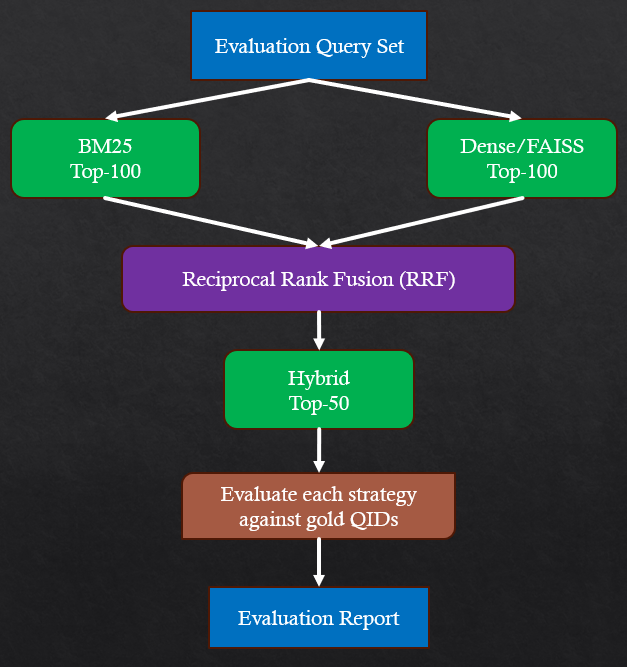
\includegraphics[
        width=0.60\textwidth,
        height=0.60\textheight,
        keepaspectratio
    ]{figures/hybrid_retrieval_pipeline.png}
    \caption{Hybrid retrieval and evaluation pipeline.}
    \label{fig:hybrid_retrieval_pipeline}
\end{figure}

\subsection{Lexical Retrieval with BM25}
First, we decided to include a lexical retrieval algorithm as part of our retrieval pipeline. Questions about historical battles often require information about exact names, locations, commanders, and tactical terms that may overlap with the corresponding battle representation. In such cases, a lexical retrieval algorithm such as BM25 can efficiently identify relevant battle documents based on term matching. It is also relatively simple and interpretable, which makes it useful as a baseline for testing.

BM25 is a widely used lexical retrieval algorithm that ranks documents according to their relevance to a given query based on term frequency, inverse document frequency, and document length normalization \citep{robertson2009bm25}. Term frequency reflects how often a query term appears in a document. Inverse document frequency gives more weight to terms that appear in fewer documents. Document length normalization is another factor in a ranking function that adjusts term frequency based on how long a document is compared to the average document length. The relevance score of a document $d$ for a query $q$ is calculated using the BM25 scoring function, as shown in Equation~\ref{eq:bm25}.

\begin{equation}
    \mathrm{BM25}(q,d) =
    \sum_{t \in q} \mathrm{IDF}(t) \cdot
    \frac{f(t,d)(k_1+1)}
    {f(t,d)+k_1\left(1-b+b\frac{|d|}{\mathrm{avgdl}}\right)}
    \label{eq:bm25}
\end{equation}
The function $\mathrm{IDF}(t)$ measures the importance of a term based on its rarity across the document collection, while $f(t,d)$ represents its frequency in document $d$. The parameter $k_1$ controls term frequency saturation, and $b$ determines the degree of document length normalization. Finally, $|d|$ denotes the document length, and $\mathrm{avgdl}$ represents the average document length across the collection.

In this work, lexical retrieval was implemented using the \texttt{BM25Okapi} algorithm provided by the Python \texttt{rank\_bm25} library \citep{brown2020rankbm25}. The implementation follows the classical BM25 ranking described by Robertson and Zaragoza (2009).

We treat each battle instance as a single retrieval document. Each structured JSON representation is serialized into a raw-text form and then tokenized by lowercasing the text and extracting tokens. The same preprocessing is applied to the user query. After the resulting corpus is indexed by the BM25 algorithm, the retrieval function computes a relevance score for every battle instance. The documents are then sorted in decreasing order of relevance, and the top-$k$ candidates are returned. Our implementation uses the default parameters provided by the library.

We index the complete JSON document rather than focusing on specific fields in order to search for lexical matches across all fields, including participants, outcomes, tactics, and others. In our implementation, BM25 does not distinguish between different JSON fields and therefore treats the entire document, including both field names and field values, as a flat token sequence. We later discuss this as a limitation and explore possible ways to make BM25 more structure-aware. This is discussed in Chapter 6, Discussion.

A successful lexical retrieval example was obtained for the query \textit{Find major battles fought in 1066 during the struggle for the English throne.} As a result, the first rank assigned by the BM25 algorithm was the Battle of Hastings (\texttt{Q83224}), with a relevance score of 44.52. Table~\ref{tab:bm25_term_contributions} shows an inspection of the relevance signals. It illustrates that the strongest signal was given by the year \textit{1066}, followed by \textit{English} and \textit{throne}. These terms were matched across different components of the structured battle representation, including metadata, participant information, and narrative content. This example demonstrates how BM25 can be effectively used for battle representations when there is substantial lexical overlap between a query and a relevant document, even without explicitly understanding the underlying nested JSON structure.
\begin{table}[htbp]
    \centering
    \caption{Contribution of query terms to the BM25 retrieval score}
    \label{tab:bm25_term_contributions}

    \small
    \renewcommand{\arraystretch}{1.3}
    \setlength{\tabcolsep}{6pt}

    \begin{tabularx}{\textwidth}{
        l
        r
        >{\raggedright\arraybackslash}X
    }
        \toprule
        \textbf{Query term} &
        \textbf{Contribution} &
        \textbf{Why it matters} \\
        \midrule

        \texttt{1066} & 14.71 &
        Exact temporal match \\

        \texttt{english} & 7.34 &
        Matches the historical and geographical context \\

        \texttt{throne} & 4.70 &
        Matches the succession conflict described in the narrative \\

        \texttt{major} & 0.67 &
        Matches the battle's scale classification \\

        \bottomrule
    \end{tabularx}
\end{table}

Although BM25 performs accurate retrieval in several cases, it still has some limitations. In particular, the algorithm relies on exact term matching and may struggle with questions that contain relevant concepts but use different wording from the corresponding passages. Furthermore, our lexical retrieval implementation does not explicitly exploit the underlying JSON structure and operates on the entire serialized document. Therefore, it may match information from less relevant fields and assign weight to tokens that are not useful for a particular query. We discuss this limitation in more detail in Chapter 6.

To address the limitation of relying on exact wording and to capture relevant concepts even when there is no direct lexical overlap, we also investigate a dense retrieval approach.
\subsection{Dense Retrieval}
As discussed in the Related Work, dense retrieval performs information retrieval by mapping queries and passages into a low-dimensional latent semantic space rather than relying on sparse keyword-matching methods such as BM25. Dense retrieval maps queries and passages into a shared embedding space and allows matches between semantically similar expressions even when they do not share the same tokens. For example, a query that mentions a \textit{surrounded army} may still match a passage that contains the term \textit{encirclement}. Similarly, a query asking about a \textit{withdrawal under pressure} may match passages containing the term \textit{retreat}. This is especially useful for battle representations that share the same tactical or narrative idea but express it in different ways. This makes dense retrieval better suited for capturing higher-level semantics and similarities between battles, and particularly useful for queries such as \textit{Find battles similar to the Battle of Cannae in which encirclement or converging attacks trapped a large enemy force and led to a catastrophic defeat}.

\citet{karpukhin2020dpr} formulates dense retrieval as a similarity comparison between independently encoded query and document representations. First, a query $q$ and a passage $p$ are mapped to dense
vectors by separate encoders $E_Q$ and $E_P$.. Their similarity is then calculated using the inner product: 

\begin{equation}
    \mathrm{sim}(q,p) = E_Q(q)^{T} E_P(p)
    \label{eq:dense-similarity}
\end{equation}


Documents with higher similarity scores are considered more relevant to the initial query. The original formulation provides a theoretical basis for our implementation, although in our approach both query and battle representation embeddings are L2-normalized before retrieval. As a result, the inner product becomes equivalent to cosine similarity:

\begin{equation}
    \mathrm{sim}(q,d) =
    \frac{e_q \cdot e_d}
    {\|e_q\| \|e_d\|}
    \label{eq:cosine-similarity}
\end{equation}


In our work, we used the \texttt{Qwen/Qwen3-Embedding-4B} embedding model provided through the ScaDS.AI OpenAI-compatible endpoint to build an index of dense vectors for our battle representations. Each battle record is represented by serializing the complete JSON object into compact text and computing a dense embedding. Embeddings were generated in batches of eight and stored as 32-bit floating-point vectors in the vector index.

The normalized battle embeddings are stored in a FAISS IndexFlatIP index \citep{douze2024faiss}, which performs exact nearest-neighbor search. When a query is executed, it is first converted into a normalized embedding vector. The query vector is then compared with all indexed battle embeddings using inner-product similarity. Finally, the top-\(k\) battle records with the highest similarity scores are returned.

However, dense retrieval also has several limitations. It may struggle to retrieve relevant battle representations based on exact entity names, rare military terms, and other specific lexical signals that are not reliably represented in the semantic embedding space. In contrast, lexical retrieval is especially effective in cases where exact or overlapping keywords are important. 

During our retrieval experiments, we observed an interesting case when testing our lexical and dense retrieval pipelines on a query asking for battles in which war elephants participated in a major attacking charge that was stopped by infantry, artillery, or reserve forces and failed to secure victory. As a result, the Battle of Khajuha (\texttt{Q4871417}), which belongs to the gold set, was ranked 3rd by the BM25 method, whereas dense retrieval placed it only in 75th position. During the analysis of term frequency and other factors used by the BM25 algorithm, we found that several terms, such as \textit{elephants}, \textit{reserve}, \textit{war}, and \textit{infantry}, made the largest contribution to the final score, which helped rank the Battle of Khajuha (\texttt{Q4871417}) so highly, as illustrated in Figure~\ref{fig:bm25_term_contributions}. Table~\ref{tab:bm25_term_evidence} additionally shows how the overall contribution of each term was calculated based on the different scoring factors. These terms directly correspond to structured information contained in the battle representation and can be found in several battle aspects, including force composition, action sequence, narrative patterns, and narrative summary.

\begin{figure}[!htbp]
    \centering
    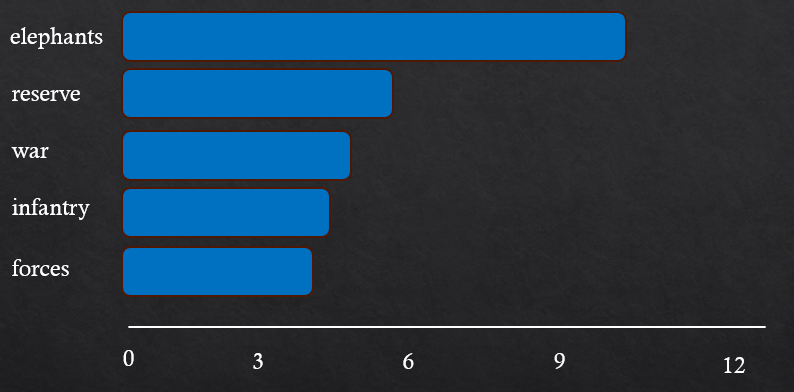
\includegraphics[
        width=0.85\textwidth,
        height=0.35\textheight,
        keepaspectratio
    ]{figures/bm25_term_contributions.png}
    \caption{Individual query-term contributions to the BM25 relevance score of a retrieved document, illustrating the relative importance of different terms in lexical retrieval.}
    \label{fig:bm25_term_contributions}
\end{figure}

\begin{table}[!htbp]
    \centering
    \caption{BM25 term-level contributions and matching evidence}
    \label{tab:bm25_term_evidence}

    \small
    \renewcommand{\arraystretch}{1.4}
    \setlength{\tabcolsep}{5pt}

    \begin{tabularx}{\textwidth}{
        >{\raggedright\arraybackslash}p{0.14\textwidth}
        >{\centering\arraybackslash}p{0.13\textwidth}
        >{\centering\arraybackslash}p{0.09\textwidth}
        >{\centering\arraybackslash}p{0.15\textwidth}
        >{\raggedright\arraybackslash}X
    }
        \toprule
        \textbf{Query term} &
        \textbf{Term frequency} &
        \textbf{IDF} &
        \textbf{BM25 contribution} &
        \textbf{Example matching evidence} \\
        \midrule

        \texttt{elephants} &
        17 &
        4.473 &
        \textbf{10.197} &
        \texttt{war elephants}; use of armored
        \texttt{war elephants}; elephant assault \\

        \midrule

        \texttt{reserve} &
        12 &
        2.440 &
        \textbf{5.364} &
        \texttt{reserve counter-attack to halt
        elephant assault}; reserve deployment \\

        \midrule

        \texttt{war} &
        15 &
        2.062 &
        \textbf{4.646} &
        \texttt{war elephants} in participants
        and military facets \\

        \midrule

        \texttt{infantry} &
        10 &
        2.062 &
        \textbf{4.428} &
        \texttt{matchlock infantry advance};
        infantry and artillery response \\

        \midrule

        \texttt{forces} &
        6 &
        2.062 &
        \textbf{4.047} &
        Reserve forces decisive in turning
        the battle \\

        \bottomrule
    \end{tabularx}
\end{table}

Since both approaches capture different relevance signals, it may be beneficial to combine them into a hybrid retrieval procedure that can potentially improve retrieval robustness. For this reason, we additionally implement a hybrid retrieval pipeline that combines the rankings from both previous retrieval methods.
\subsection{Hybrid Retrieval}
As discussed above, lexical and dense retrieval capture different types of relevance signals. Lexical retrieval is particularly effective at finding exact matches between a query and a battle representation, while dense retrieval can identify semantically related records even when the query and the relevant representation use different wording. This motivates the use of a hybrid retrieval pipeline that combines the rankings from both methods.

The scores produced by BM25 and dense retrieval are not directly comparable because they use different scoring functions and operate on different scales. We therefore combine the two rankings using Reciprocal Rank Fusion (RRF). RRF combines the rankings based on the position of each battle in the individual result lists. 
For every candidate battle $d$, its BM25 and dense ranks are converted into reciprocal-rank contributions using $1/(k + \mathrm{rank})$.
A single fused score is then obtained using the following formula, as shown in Equation~\eqref{eq:rrf}:

\begin{equation}
    \mathrm{RRF}(d) =
    \sum_{r} \frac{1}{k + \mathrm{rank}_r(d)}
    \label{eq:rrf}
\end{equation}

Here, $r$ denotes the retrieval system and $k$ is a smoothing constant, which was set to 60 in our implementation. A battle that is ranked highly by both lexical and dense retrieval receives two relatively large reciprocal-rank contributions, one from each retrieval system. After an RRF score has been calculated for every candidate battle, the candidates are sorted in descending order of their fused RRF scores to obtain the final hybrid ranking. In our hybrid retrieval pipeline, the top 100 results from BM25 and the top 100 results from dense retrieval are used as the candidate pool. After RRF fusion, only the highest-ranked 50 battles are retained as the final hybrid retrieval results. 

As an example, let us take the query \textit{Find a major battle fought in BCE during the Second Punic War in which Carthage fought Rome}. Lexical retrieval ranks the Battle of Zama (\texttt{Q200056}) 23rd, while dense retrieval ranks this battle 5th. The fused score is calculated as
$\frac{1}{60+23} + \frac{1}{60+5} \approx 0.02743$. The same RRF calculation is applied to every unique candidate battle appearing in the top 100 BM25 results or the top 100 dense-retrieval results. After sorting the obtained results by decreasing RRF score, 10 battles receive higher fused scores than the Battle of Zama, so the Battle of Zama is ranked 11th in the hybrid pipeline. 
\section{Answer Generation}
According to RQ3, we aim to identify how does the use of structured battle representations as external evidence affect LLM-based question-answering quality compared with direct LLM querying and raw-text augmentation? For this purpose, after retrieval, the final stage of the pipeline generates the set of battles that satisfy a query and compares three answer-generation configurations: a baseline LLM without retrieved context, an LLM augmented with structured JSON battle records, and an LLM augmented with the corresponding raw Wikipedia texts. The same underlying language model and generation configuration are used across all three settings. The information provided to the LLM differs depending on the configuration.

In addition, we conduct two types of generation experiments. Oracle-context generation evaluates generation quality in isolation from retrieval, where the model is provided with a predefined list of candidate battles that includes gold battles and negative examples. The end-to-end RAG experiment evaluates generation together with retrieval; instead of receiving a predefined candidate set, the model uses the battles returned by the hybrid retrieval pipeline. Table~\ref{tab:oracle_vs_e2e} shows the comparison between 2 generation experiments in terms of their goal, provided context, exposition of golden set, and use of retrieval pipeline.
\begin{table}[htbp]
    \centering
    \caption{Comparison of oracle-context and end-to-end experiments}
    \label{tab:oracle_vs_e2e}

    \small
    \renewcommand{\arraystretch}{1.4}
    \setlength{\tabcolsep}{5pt}

    \begin{tabular}{
        p{0.24\textwidth}
        p{0.32\textwidth}
        p{0.32\textwidth}
    }
        \toprule
        &
        \textbf{Oracle-context experiment} &
        \textbf{End-to-end experiment} \\
        \midrule

        Candidate battles &
        Gold + predefined negatives &
        Returned by hybrid retrieval \\
        \midrule

        Gold present in context? &
        \textbf{Yes} &
        \textbf{No} \\
        \midrule

        Baseline receives candidates? &
        \textbf{Yes} &
        \textbf{No} \\
        \midrule

        JSON context &
        Candidate JSON records &
        Retrieved JSON records \\
        \midrule

        Raw-text context &
        Candidate article texts &
        Retrieved article texts \\
        \midrule

        Main question &
        Can the LLM select the right battles given correct candidates? &
        Can the complete retrieval and generation pipeline answer correctly? \\
        \midrule

        Retrieval errors included? &
        \textbf{No} &
        \textbf{Yes} \\

        \bottomrule
    \end{tabular}
\end{table}
\subsection{Oracle-context generation}
In the Oracle-context generation experiment, our goal is to evaluate the ability of the model to choose the correct set of battles from a provided list of candidate battles that contains both gold battles and closed-set negatives. All three configurations, including the baseline LLM, JSON-augmented LLM, and raw-text-augmented LLM, receive the same set of candidate battles in the context. Figure~\ref{fig:closed_set_baseline} shows how the process works for the baseline configuration. The model receives only the instruction to answer the question using its internal knowledge and select relevant battles from the candidate pool.

\begin{figure}[!htbp]
    \centering
    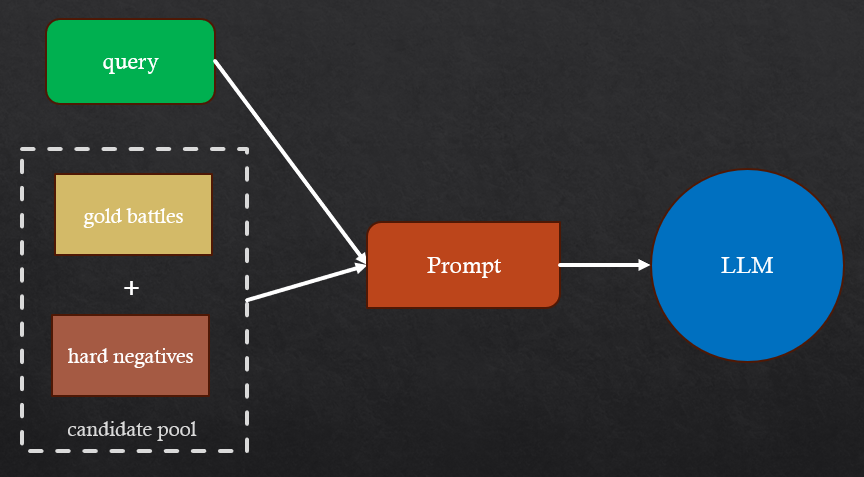
\includegraphics[
        width=0.75\textwidth,
        keepaspectratio
    ]{figures/closed_set_baseline.png}
    \caption{Closed-set baseline configuration.}
    \label{fig:closed_set_baseline}
\end{figure}

\begin{figure}[!htbp]
    \centering
    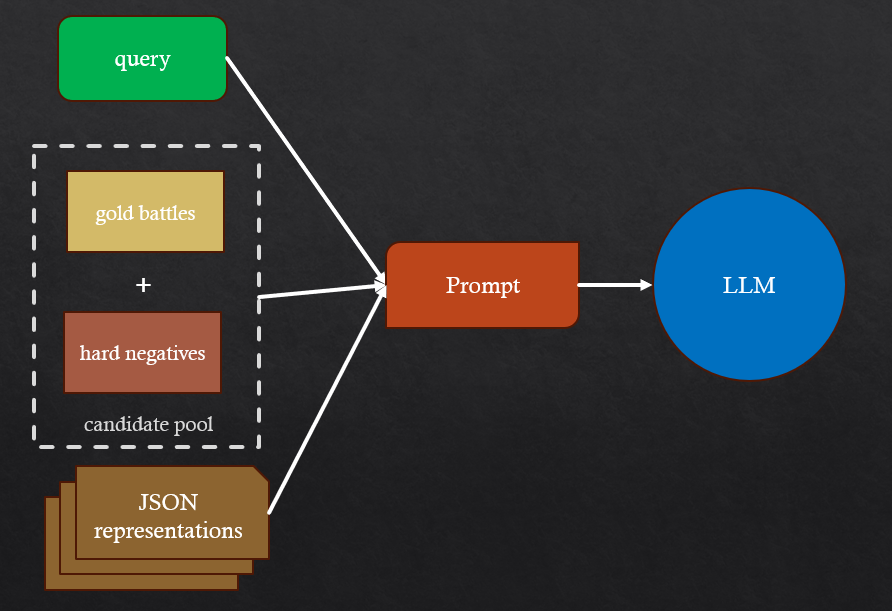
\includegraphics[
        width=0.75\textwidth,
        keepaspectratio
    ]{figures/closed_set_json.png}
    \caption{Closed-set JSON-augmented configuration.}
    \label{fig:closed_set_json}
\end{figure}

As shown in Figure~\ref{fig:closed_set_json}, the JSON-augmented configuration additionally receives structured battle representations as context. These structured representations include battle records from both the gold set and the closed-set negatives. The instruction is similar: the model must choose relevant battles from the provided candidate list, but this time it is prohibited from using its internal knowledge and must answer only using the provided context. This constraint is introduced to isolate the contribution of external context and determine whether the supplied battle representations contain sufficient information to produce the correct set of relevant battles. Without this constraint, it would be difficult to determine whether the model’s answer was based on the provided context or on its parametric memory. The same evidence-use restriction is applied to the raw-text-augmented configuration to enable a controlled comparison. A similar pipeline for the raw-text-augmented configuration is illustrated in Figure~\ref{fig:closed_set_raw_text}.

\begin{figure}[!htbp]
    \centering
    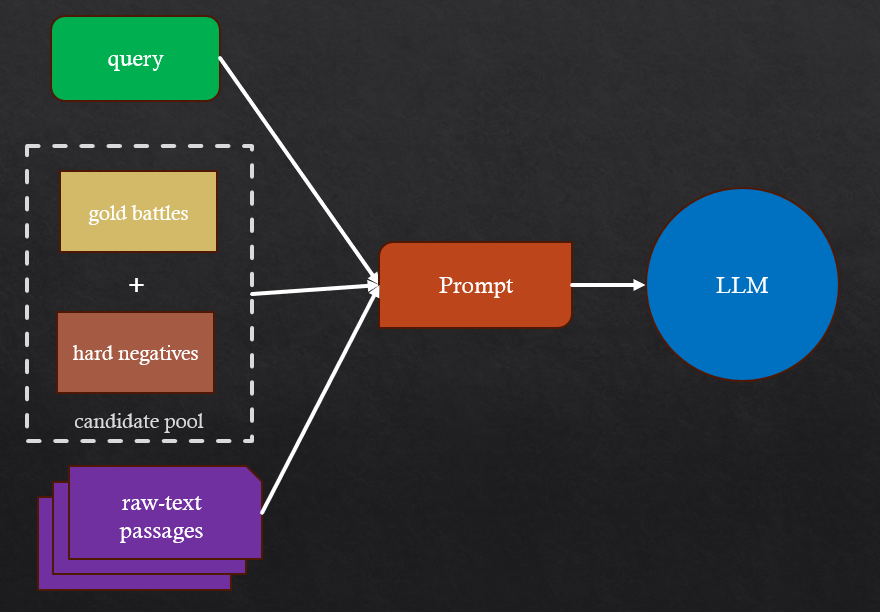
\includegraphics[
        width=0.85\textwidth,
        keepaspectratio
    ]{figures/closed_set_raw_text.png}
    \caption{Closed-set raw-text-augmented configuration.}
    \label{fig:closed_set_raw_text}
\end{figure}

\subsection{End-to-end generation}
In the end-to-end RAG experiment, our goal is to evaluate the complete retrieval and answer-generation pipeline under realistic conditions, where the relevant battles are not guaranteed to be present in the model context. Unlike the oracle-context experiment, the baseline LLM does not receive a predefined candidate set. Instead, it receives only the original query and must identify matching battles using its internal knowledge. The JSON-augmented and raw-text-augmented configurations, in contrast, receive battle records selected by the hybrid retrieval pipeline. For each query, the top-$k$ retrieved battles are used as context, so the final answer depends on both retrieval quality and the model’s ability to correctly interpret the retrieved evidence. All three configurations are shown in Figure~\ref{fig:e2e_baseline}, Figure~\ref{fig:e2e_rag_json} and Figure~\ref{fig:e2e_rag_rawtext}.

\begin{figure}[!htbp]
    \centering
    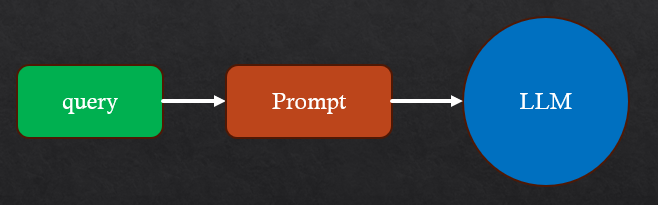
\includegraphics[
        width=0.85\textwidth,
        keepaspectratio
    ]{figures/e2e_rag_baseline.png}
    \caption{End-to-end baseline model configuration.}
    \label{fig:e2e_baseline}
\end{figure}

\begin{figure}[!htbp]
    \centering
    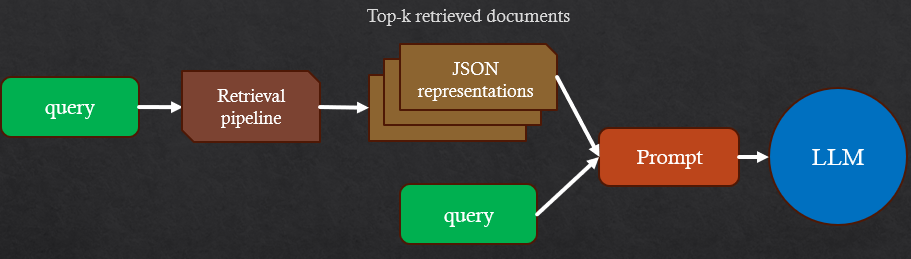
\includegraphics[
        width=\textwidth,
        keepaspectratio
    ]{figures/e2e_rag_json.png}
    \caption{End-to-end JSON-augmented model configuration.}
    \label{fig:e2e_rag_json}
\end{figure}

\begin{figure}[!htbp]
    \centering
    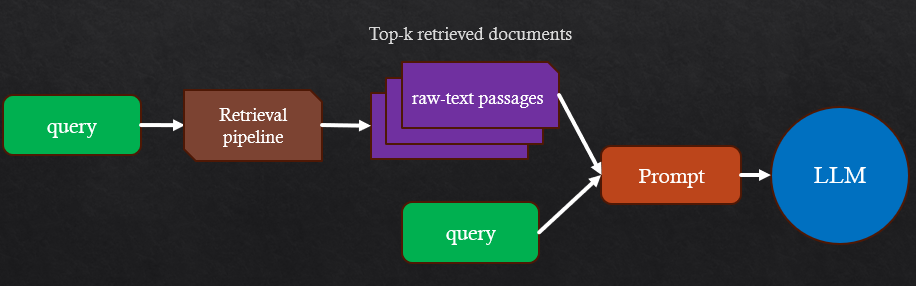
\includegraphics[
        width=\textwidth,
        keepaspectratio
    ]{figures/e2e_rag_rawtext.png}
    \caption{End-to-end raw-text-augmented model configuration.}
    \label{fig:e2e_rag_rawtext}
\end{figure}


In the JSON-augmented configuration, the model receives the generation query and the top-$k$ structured battle passages retrieved by the hybrid retrieval pipeline. The model is instructed to use the battle records as evidence and not to rely on its internal knowledge. It may return only battles that occur in the retrieved context and are directly supported by it. The raw-text-augmented configuration follows the same principle, but the retrieved context consists of the corresponding Wikipedia article text instead of structured battle representations. For the latter two configurations, the same restriction against using the model’s internal knowledge is applied in order to compare the augmented configurations under equivalent evidence conditions.

The end-to-end setup is designed to evaluate the full RAG process, including both retrieval and generation, and to analyze how the model performs across all three configurations without access to a predefined candidate battle pool.

In the next chapter, we discuss the experimental setup in detail, including the set of testing queries, evaluation metrics, and experiment design.
\chapter{Experimental Design}
This chapter presents the experimental design used to evaluate the main components of our system. We first describe the construction of our query set, including query types, difficulty levels, context rarity, gold battles, and closed-set negatives. We then present three groups of experiments: the Oracle-context generation experiment for evaluating generation in isolation, the retrieval experiment for comparing lexical, dense, and hybrid retrieval, and the end-to-end RAG experiment for evaluating the complete retrieval and generation pipeline under more realistic conditions.
\section{Query Set}
To prepare the query set, we first designed a JSON structure for each query object so that it could be processed during the experimental stage and later results analysis. 

\begin{minipage}{\textwidth}
\begin{lstlisting}[
    style=jsonstyle,
    caption={Illustrative evaluation query JSON object.},
    label={lst:evaluation_query_example}
]
{
  "query_id": "q001",
  "query": "Find major battles fought in 1066 during the struggle for the English throne.",
  "generation_query": "...",
  "query_type": "Temporal",
  "query_structure": "Conjunctive",
  "gold_battles": {
    "Q1113659": "Battle of Fulford",
    "Q203225": "Battle of Stamford Bridge",
    "Q83224": "Battle of Hastings"
  },
  "closed_set_negatives": {
    "Q222013": "Battle of Bosworth Field",
    "Q188495": "Battle of Agincourt",
    "Q27759": "Battle of Crecy",
    "Q201692": "Battle of Poitiers",
    "Q499626": "Battle of Stirling Bridge",
    "Q4590555": "Battle of Loudoun Hill"
  },
  "explanation": "...",
  "query_difficulty": "easy",
  "context_rarity": "common"
}
\end{lstlisting}
\end{minipage}
Listing~\ref{lst:evaluation_query_example} shows a complete example of a query JSON object, including all relevant fields such as \texttt{query\_id}, \texttt{query}, \texttt{query\_type}, \texttt{gold\_battles}, \texttt{closed\_set\_negatives}, and \texttt{context\_rarity}. Each query is identified by \texttt{query\_id}. The question provided to the LLM is contained in the \texttt{query} field. Another field, \texttt{generation\_query}, is used as input to the LLM in oracle-context experiments, where the model is additionally aware of the set of candidate battles from which it must choose. The \texttt{query\_type} field defines the query category. There are six main query types: Temporal, Participant-related, Spatial/Terrain, Weapon/Unit-related, Outcome-related, and Narrative/Tactical, as well as one additional category, Similarity, which is tested separately in some experiments. Table~\ref{tab:query_types} provides additional information about the query types, including a description of each category, the number of questions used, and an example query. In total, there are 102 queries: 92 from the six main query types and 10 from the Similarity category.
\begin{table}[htbp]
\centering
\caption{Overview of evaluation query types}
\label{tab:query_types}

\scriptsize
\renewcommand{\arraystretch}{1.3}
\setlength{\tabcolsep}{3pt}

\begin{tabular}{p{0.16\textwidth} p{0.27\textwidth} c p{0.36\textwidth}}
\toprule
\textbf{Query type} &
\textbf{Description} &
\textbf{Count} &
\textbf{Example query} \\
\midrule

\textbf{Temporal} &
Queries involving years, historical periods, campaigns, or chronological relationships. &
10 &
\textit{Find major battles fought in 1066 during the struggle for the English throne.} \\
\midrule

\textbf{Spatial / Terrain} &
Queries involving geographical locations, terrain features, and battlefield conditions. &
13 &
\textit{Find battles where a smaller defending force exploited a narrow or restricted approach to reduce the attacking army's numerical advantage.} \\
\midrule

\textbf{Participant-related} &
Queries concerning commanders, armies, alliances, and relationships between forces. &
15 &
\textit{Find major battles in which Hannibal personally commanded Carthaginian forces against Roman armies.} \\
\midrule

\textbf{Outcome-related} &
Queries focusing on battle results, defeats, retreats, and strategic consequences. &
12 &
\textit{Find battles where the losing army was surrounded or trapped and then suffered catastrophic destruction rather than making an orderly withdrawal.} \\
\midrule

\textbf{Weapon / Unit-related} &
Queries concerning weapons, military units, technologies, and tactical roles. &
20 &
\textit{Find battles where war elephants were deployed prominently but failed to secure victory for the army using them.} \\
\midrule

\textbf{Narrative / Tactical} &
Queries describing tactical patterns, event sequences, and battlefield maneuvers. &
22 &
\textit{Find battles where a successful encirclement trapped a large enemy force and caused catastrophic defeat.} \\
\midrule

\textbf{Similarity} &
Queries comparing battles based on tactical, operational, terrain, or outcome characteristics. &
10 &
\textit{Find battles similar to Cannae in which encirclement or converging attacks trapped a large enemy force and led to catastrophic defeat.} \\
\midrule

\textbf{Total} &
&
\textbf{102} &
\\

\bottomrule
\end{tabular}
\end{table}
The \texttt{gold\_battles} field contains a JSON object that maps each battle's Wikidata ID to its corresponding name. As illustrated in Listing~\ref{lst:evaluation_query_example}, the golden battles for the query \textit{Find major battles fought in 1066 during the struggle for the English throne.} are Battle of Fulford(\texttt{Q1113659}), Battle of Stamford Bridge(\texttt{Q203225}), Battle of Hastings(\texttt{Q83224}). The \texttt{closed\_set\_negatives} field is used mainly for oracle-context generation experiment to form a battle set given to the model that contains both \texttt{golden\_battles} and similar negative battles aimed to confuse the model. In the next field \texttt{query\_difficulty} we define 3 difficulty levels such as easy, medium, hard based on the amount of reasoning required. Easy queries are based on explicit factual clues, medium require knowledge of several attributes or interpreting a tactical or causal pattern, while hard queries need more complex semantic reasoning over longer event sequences or abstract similarities between battles. Queries were also characterized by \texttt{context\_rarity}. This field reflects how common or obscure the referenced battle and the related information are likely to be in general knowledge. The motivation was to reduce the advantage of a baseline LLM, which might easily answer questions about well-known battles from its parametric memory but may have more difficulty answering questions about rare battles. Rare-context queries therefore focus on less famous battles.

The complete benchmark of 102 queries was constructed with the assistance of the GPT-5.6 Sol model using a corpus-grounded generation process. We did not ask the model to generate queries based on its own historical knowledge. Instead, information about historical battles was provided in smaller batches of around 1,000 battle records at a time. These records represented compact battle structures capturing the most important factual and narrative information needed for the model to reason over them and use this information for query generation. They were constructed based on our complete JSON battle knowledge base, KB2.

For each batch, GPT-5.6 Sol was instructed to identify meaningful factual and narrative properties, shared patterns, and formulate query objects according to the predefined structure shown in Listing~\ref{lst:evaluation_query_example}. The model was additionally instructed to generate queries of different types described above and to include both common and rare battles. In the output, the model also proposed a gold set containing Wikidata QIDs and names of relevant battles, as well as a set of closed-set negatives. For hard negatives, the model selected battles that were similar to the gold battles but failed one or several essential conditions of the query. An explanation field was also added, where the model briefly described why the gold-set battles were selected. Overall, the query-set generation process is illustrated in Figure~\ref{fig:query_set_generation}.

\begin{figure}[!htbp]
    \centering
    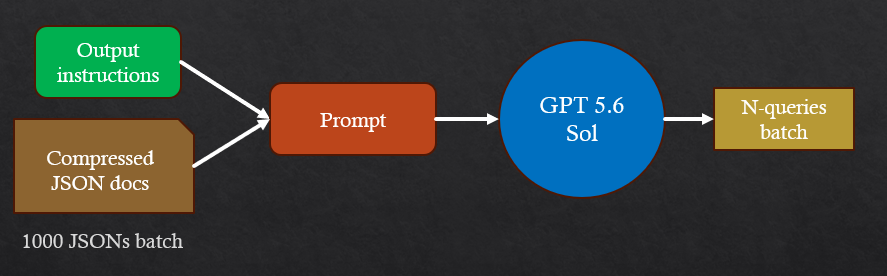
\includegraphics[
        width=\textwidth,
        keepaspectratio
    ]{figures/query_set_generation.png}
    \caption{Evaluation query set generation pipeline.}
    \label{fig:query_set_generation}
\end{figure}

\section{Oracle-context Generation Experiment}
As described in Chapter 3.6, the Oracle-context generation experiment aims to evaluate the ability of the model to choose the correct set of battles from a provided list of candidate battles consisting of both gold battles and closed-set negatives. The process for all three LLM configurations including the baseline LLM, JSON-augmented LLM, and raw-text-augmented LLM was illustrated in detail in Figure~\ref{fig:closed_set_baseline}, Figure~\ref{fig:closed_set_json} and Figure~\ref{fig:closed_set_raw_text}. For all experiments, GPT-OSS-120B is used again. In this experiment, there is no retrieval step, so we evaluate generation performance in isolation. The baseline LLM does not receive any external context and performs reasoning using only its internal knowledge. In the JSON-augmented and raw-text-augmented configurations, the LLM receives either JSON battle representations or raw-text Wikipedia articles, respectively. The provided battle instances include both battles from the gold set and battles from the closed-set negative set. We use KB2 as the battle knowledge corpus from which battle representations are provided to the JSON-augmented model. For additional analysis, we also include results from a JSON-augmented model that received battle representations from KB1 to evaluate how the LLM Verification and Regeneration step improved the structured battle knowledge base.

To gain more insight into generation performance and the differences between the three configurations, we divide the experiment into three parts. In the first part, we analyze the overall generation performance and compare the results obtained using KB1 and KB2. In the second part, we analyze generation performance for common and rare battles separately, by filtering the initial query set. In the third part, we evaluate the LLM configurations across different query types to examine how query type affects the ability of the LLM to provide accurate answers. Similarity queries are excluded from this overall comparison and evaluated separately. Table~\ref{tab:generation_experiment_parts} illustrates all three parts of the experiment, including their aims, testing subjects, and descriptions.
\begin{table}[htbp]
    \centering
    \caption{Overview of the generation evaluation experiments}
    \label{tab:generation_experiment_parts}

    \small
    \renewcommand{\arraystretch}{1.5}
    \setlength{\tabcolsep}{4pt}

    \begin{tabular}{
        >{\raggedright\arraybackslash}p{0.15\textwidth}
        >{\raggedright\arraybackslash}p{0.22\textwidth}
        >{\raggedright\arraybackslash}p{0.29\textwidth}
        >{\raggedright\arraybackslash}p{0.26\textwidth}
    }
        \toprule
        \textbf{Part} &
        \textbf{Aim} &
        \textbf{Testing subjects} &
        \textbf{Description} \\
        \midrule

        \textbf{1. Overall} &
        Compare overall generation performance across model configurations. &
        Baseline; Raw-text-augmented; JSON-augmented (KB2);
        JSON-augmented (KB1) &
        Evaluated across the 92 main queries using generation metrics.
        KB1 is included to assess the effect of the Verification
        and Regeneration step. \\
        \midrule

        \textbf{2. Common vs. Rare} &
        Analyze how battle rarity affects generation performance. &
        Common queries; Rare queries &
        Performance is compared separately for common and
        rare battle queries. \\
        \midrule

        \textbf{3. Query Type} &
        Compare generation performance across semantic query categories. &
        Temporal; Participant-related; Spatial/Terrain;
        Weapon/Unit-related; Outcome-related; Narrative/Tactical;
        Similarity &
        Performance is analyzed separately for each query type.
        Similarity is evaluated on its separate 10-query set. \\

        \bottomrule
    \end{tabular}
\end{table}
To evaluate generation performance, we use four main metrics: precision, recall, F1, and exact match. The metrics are computed independently for each query and then macro-averaged across all evaluated queries. Additionally, we count the number of parse errors and run errors.

The model is instructed to follow a specific JSON output format, which is parsed after generation. The returned battle QIDs are used for quantitative evaluation. Duplicate predicted QIDs are removed before the metrics are calculated. For each query, precision and recall are computed by comparing the predicted QID set with the corresponding gold QID set, while F1 is calculated as their harmonic mean. Exact match is assigned a value of 1 only if the predicted set of battles is identical to the complete gold set, and 0 otherwise. We use the \texttt{battle\_names} and \texttt{explanations} fields for debugging purposes and overall analysis. Responses that cannot be parsed into the expected JSON structure or that contain invalid QIDs are recorded as parse errors and receive zero scores for the generation metrics. If the model encounters a failure during execution, we record it separately as a run error.
\section{Retrieval Experiment}
The methodology and implementation of the three retrieval pipelines, lexical, dense, and hybrid retrieval, were previously discussed in Chapter 3.5. In this section, we discuss the retrieval experiments used to compare these approaches. The retrieval experiment aims to evaluate the retrieval step in isolation and determine how well each retrieval algorithm ranks battle instances from our historical battle knowledge base for a given query. All three strategies were evaluated using the same set of 102 raw-text queries and compared against the corresponding gold sets of relevant historical battles. For each query, the BM25 and dense retrieval algorithms independently returned the top 100 candidate battles, ranked according to their retrieval scores. The two ranked lists were then combined using Reciprocal Rank Fusion, producing a hybrid ranking that was limited to the top 50 battles.

We used six metrics to evaluate the performance of each retrieval algorithm: Recall@10, Recall@20, Recall@50, Mean Reciprocal Rank (MRR), Mean Average Precision at 10 (MAP@10), and normalized Discounted Cumulative Gain at 10 (nDCG@10). Recall@k measures the proportion of relevant battle records retrieved among the top-$k$ results. MRR evaluates the rank position of the first relevant battle. MAP@10 assesses how highly relevant battle records are ranked among the top 10 candidates. Finally, nDCG@10 evaluates ranking quality by assigning higher importance to relevant battles appearing at earlier positions. A detailed description and mathematical formulation of the metrics is provided in Table~\ref{tab:retrieval_metrics}. Binary relevance labels were used: battles included in the query-specific gold set were treated as relevant, while all other battles were treated as non-relevant. All metrics were computed independently for each query and then macro-averaged across the query set, giving each query equal weight.
\begin{table}[htbp]
    \centering
    \caption{Retrieval evaluation metrics and their interpretations}
    \label{tab:retrieval_metrics}

    \small
    \renewcommand{\arraystretch}{1.8}
    \setlength{\tabcolsep}{6pt}

    \begin{tabular}{
        >{\raggedright\arraybackslash}p{0.13\textwidth}
        >{\centering\arraybackslash}p{0.30\textwidth}
        >{\raggedright\arraybackslash}p{0.43\textwidth}
    }
        \toprule
        \textbf{Metric} &
        \textbf{Formula} &
        \textbf{Interpretation} \\
        \midrule

        \textbf{Recall@k} &
        $\displaystyle
        \mathrm{Recall@k} =
        \frac{|R_k \cap G|}{|G|}
        $ &
        Measures the proportion of relevant battles retrieved
        within the top $k$ results. \\
        \midrule

        \textbf{MRR} &
        $\displaystyle
        MRR = \frac{1}{N}
        \sum_{i=1}^{N}
        \frac{1}{rank_i}
        $ &
        Measures how early the first relevant battle appears
        in the ranking. \\
        \midrule

        \textbf{MAP@10} &
        $\displaystyle
        MAP@10 = \frac{1}{N}
        \sum_{i=1}^{N} AP_i@10
        $ &
        Measures how highly and consistently relevant battles
        are ranked within the top 10 results. \\
        \midrule

        \textbf{nDCG@10} &
        $\displaystyle
        nDCG@10 =
        \frac{DCG@10}{IDCG@10}
        $ &
        Measures ranking quality while giving greater
        importance to relevant battles appearing at
        higher ranks. \\

        \bottomrule
    \end{tabular}
\end{table}
The experiments were again divided into four parts, as shown in Table~\ref{tab:retrieval_experiment_parts}. First, we report the overall retrieval performance across the complete query set and compare the results obtained using the KB1 and KB2 battle corpora. In the second experiment, we analyze retrieval quality separately for queries describing common and rare battles. Finally, the queries are filtered by \texttt{query\_type}, and retrieval performance is evaluated separately across the different query types.
\begin{table}[htbp]
    \centering
    \caption{Overview of the retrieval evaluation experiments}
    \label{tab:retrieval_experiment_parts}

    \small
    \renewcommand{\arraystretch}{1.5}
    \setlength{\tabcolsep}{4pt}

    \begin{tabular}{
        >{\raggedright\arraybackslash}p{0.15\textwidth}
        >{\raggedright\arraybackslash}p{0.22\textwidth}
        >{\raggedright\arraybackslash}p{0.29\textwidth}
        >{\raggedright\arraybackslash}p{0.26\textwidth}
    }
        \toprule
        \textbf{Part} &
        \textbf{Aim} &
        \textbf{Testing subjects} &
        \textbf{Description} \\
        \midrule

        \textbf{1. Overall Performance} &
        Compare the overall retrieval performance of
        the three retrieval algorithms. &
        BM25; Dense; Hybrid &
        Performance is evaluated across the complete query
        set using Recall@10, Recall@20, Recall@50, MRR,
        MAP@10, and nDCG@10. \\
        \midrule

        \textbf{2. Common vs. Rare} &
        Analyze how battle rarity affects retrieval quality. &
        Common queries; Rare queries &
        Retrieval performance is compared separately for
        queries concerning common and rare battles. \\
        \midrule

        \textbf{3. Query Type} &
        Compare retrieval performance across different
        semantic query categories. &
        Temporal; Participant-related; Spatial/Terrain;
        Weapon/Unit-related; Outcome-related;
        Narrative/Tactical; Similarity &
        Retrieval metrics are analyzed separately for each
        query type to identify differences between BM25,
        dense, and hybrid retrieval. \\

        \bottomrule
    \end{tabular}
\end{table}
Listing~\ref{lst:retrieval_rare_results} shows an example of the JSON output produced by the retrieval pipeline when it was run on a set of rare queries.

\begin{minipage}{\textwidth}
\begin{lstlisting}[
    style=jsonstyle,
    caption={Example of the JSON output containing retrieval evaluation metrics for BM25, dense, and hybrid retrieval strategies on rare queries. Metric values are rounded to three decimal places.},
    label={lst:retrieval_rare_results}
]
{
  "bm25": {
    "Recall@10": 0.508,
    "Recall@20": 0.586,
    "Recall@50": 0.651,
    "MRR": 0.543,
    "MAP@10": 0.428,
    "nDCG@10": 0.475
  },
  "dense": {
    "Recall@10": 0.505,
    "Recall@20": 0.565,
    "Recall@50": 0.596,
    "MRR": 0.521,
    "MAP@10": 0.425,
    "nDCG@10": 0.468
  },
  "hybrid": {
    "Recall@10": 0.583,
    "Recall@20": 0.615,
    "Recall@50": 0.727,
    "MRR": 0.572,
    "MAP@10": 0.470,
    "nDCG@10": 0.526
  }
}
\end{lstlisting}
\end{minipage}

\section{End-to-end RAG Experiment}
Following the description of the generation experiments in Chapter 3.6, the end-to-end RAG experiment evaluates the complete pipeline, including both retrieval and answer-generation steps. Unlike the Oracle-context experiment, the set of candidate battles to choose from is not provided in advance. Instead, the retrieval pipeline first selects the top-$k$ battle records from the knowledge base, and these retrieved records are then passed to the generation stage. We use the hybrid retrieval pipeline for the retrieval step. We again compare three LLM configurations: the baseline LLM, the raw-text-augmented LLM, and the JSON-augmented LLM. The baseline LLM receives only the original query and relies on its internal knowledge, while the JSON-augmented and raw-text-augmented configurations receive retrieved JSON battle representations or the corresponding raw Wikipedia texts as external context. We additionally analyze the performance of the augmented models for different values of $k$, representing different numbers of retrieved battle instances. The final performance in this experiment depends on both retrieval quality and the model’s ability to correctly interpret the retrieved evidence.

The end-to-end RAG experiment is divided into three parts to test different aspects of the complete pipeline across different query categories and configurations. In the first part, we test the effect of different values of $k$, representing different numbers of retrieved battle instances provided by the hybrid retrieval algorithm. By default, it returns a ranked list of the top 50 battle records for each query. However, providing 50 JSON representations to the LLM may introduce a substantial amount of irrelevant information and increase the context length. Previous work has shown that LLMs may struggle to effectively utilize relevant information in long contexts, particularly when it appears in the middle of the input prompt \citep{liu2024lostinthemiddle}. Therefore, we investigate different $k$-values representing the top-ranked battles supplied to the LLM. The goal is to find an optimal retrieval depth that balances the presence of relevant battles with answer accuracy.

We use the same set of metrics as in the Oracle-context experiment, including precision, recall, F1, exact match, and error rate. To complement the retrieval quality analysis, we additionally adopt two evaluation metrics inspired by the RAGAS framework: faithfulness and context relevance \citep{es2024ragas}. Faithfulness measures how well the statements generated by the LLM are supported by the retrieved context, while context relevance evaluates how much of the retrieved information is relevant to answering the original query. These additional metrics help assess the quality of the context provided to the LLM and its usefulness during answer generation.

In our implementation, the metrics are computed in the following way. For each predicted battle, the generated explanation is compared against the corresponding JSON battle representation, and the LLM evaluator marks it as supported only if all factual claims can be inferred from the JSON file. The faithfulness score is then computed as the proportion of fully supported explanations. To evaluate context relevance, each JSON battle representation supplied to the generation model is independently judged as relevant or irrelevant to the query. The context relevance score is computed as the proportion of relevant JSON representations that are useful for answering the question. For both metrics, the LLM evaluator receives only the provided query, the generated explanation, and the retrieved JSON context. 

In our experiments, we investigated how different values of $k$ affect the performance and error rate of the augmented models. In addition, we evaluated model performance separately for queries involving common and rare battles and across different query types.
\chapter{Experimental Results}
In this chapter we discuss Experiment Results, specifically for Retrieval, Oracle-context generation and End-to-end RAG experiments. 
\section{Retrieval Results}
As previously discussed in Chapter 4.3, we conducted three sub-experiments to evaluate different aspects of retrieval quality and performance. First, we report the overall retrieval results across the complete set of 102 queries and compare retrieval performance when using the KB1 and KB2 battle corpora. Second, we focus on queries involving common and rare battles and analyze how context rarity affects the performance of each retrieval strategy. Finally, we investigate how retrieval performance differs across different query types.
\subsection{Overall Retrieval Performance}
Table~\ref{tab:overall_retrieval_performance} shows the overall retrieval performance across all 102 queries. Additionally, we compare retrieval performance separately using the KB1 and KB2 battle corpora. Figure~\ref{fig:overall_retrieval_comparison} show Recall@10/20/50, MRR, MAP@10 and nDCG@10 scores for the three retrieval pipelines: lexical, dense, and hybrid retrieval. Additional labels distinguish the results obtained using KB1 (bars on the left) from those obtained using KB2 (bars on the right). Recall scores remain similar across the two knowledge base versions, suggesting that KB2 does not provide a substantial retrieval advantage over KB1. Dense retrieval improves Recall over BM25 by approximately 9.0\% on average, while hybrid retrieval further improves Recall over dense retrieval by approximately 1.4\%. The higher recall of dense retrieval is consistent with its ability to capture semantic similarity beyond exact lexical overlap. 

\begin{figure}[!htbp]
    \centering

    % Row 1
    \begin{subfigure}[t]{0.48\textwidth}
        \centering
        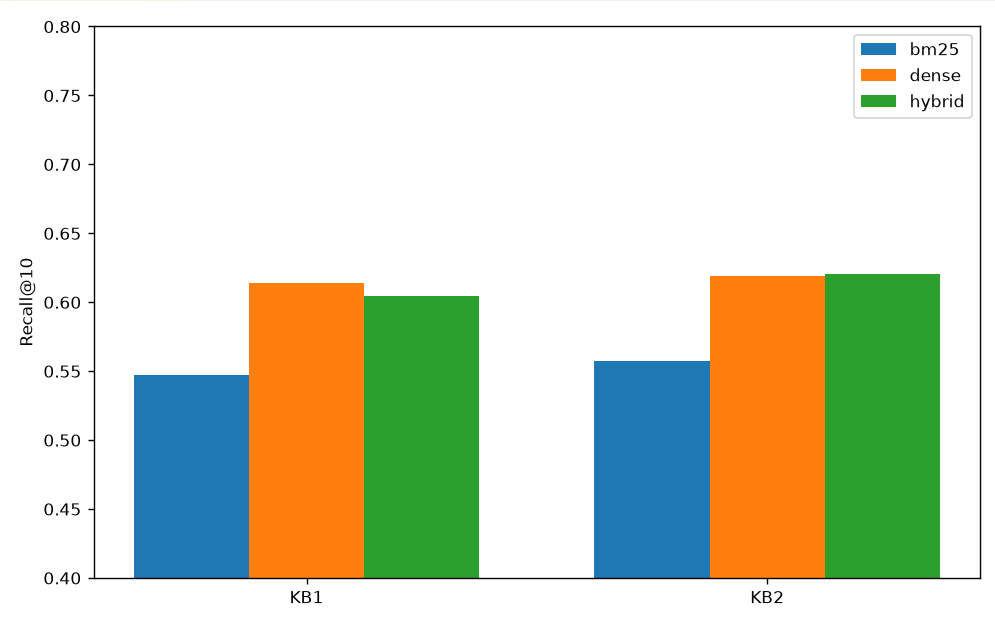
\includegraphics[width=\linewidth]{figures/overall_retrieval_recall10.png}
        \caption{Recall@10}
        \label{fig:overall_retrieval_recall10}
    \end{subfigure}
    \hfill
    \begin{subfigure}[t]{0.48\textwidth}
        \centering
        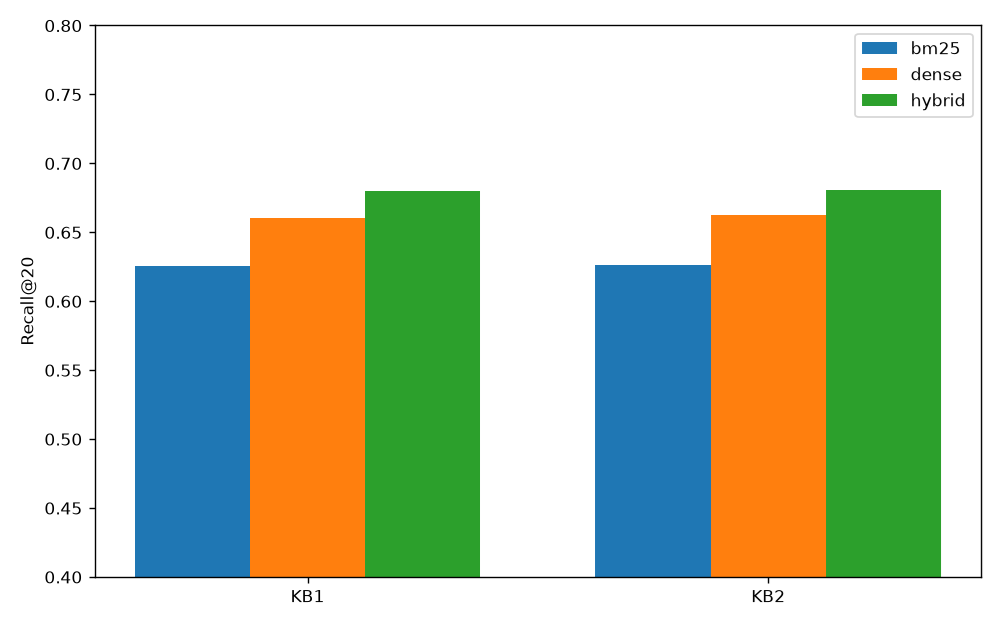
\includegraphics[width=\linewidth]{figures/overall_retrieval_recall20.png}
        \caption{Recall@20}
        \label{fig:overall_retrieval_recall20}
    \end{subfigure}

    \vspace{0.2cm}

    % Row 2
    \begin{subfigure}[t]{0.48\textwidth}
        \centering
        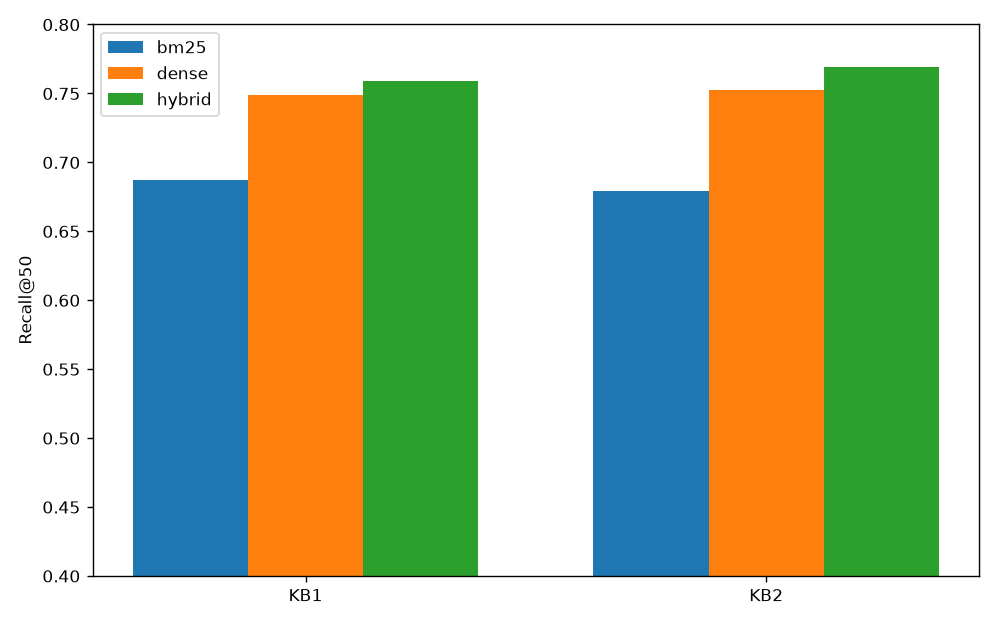
\includegraphics[width=\linewidth]{figures/overall_retrieval_recall50.png}
        \caption{Recall@50}
        \label{fig:overall_retrieval_recall50}
    \end{subfigure}
    \hfill
    \begin{subfigure}[t]{0.48\textwidth}
        \centering
        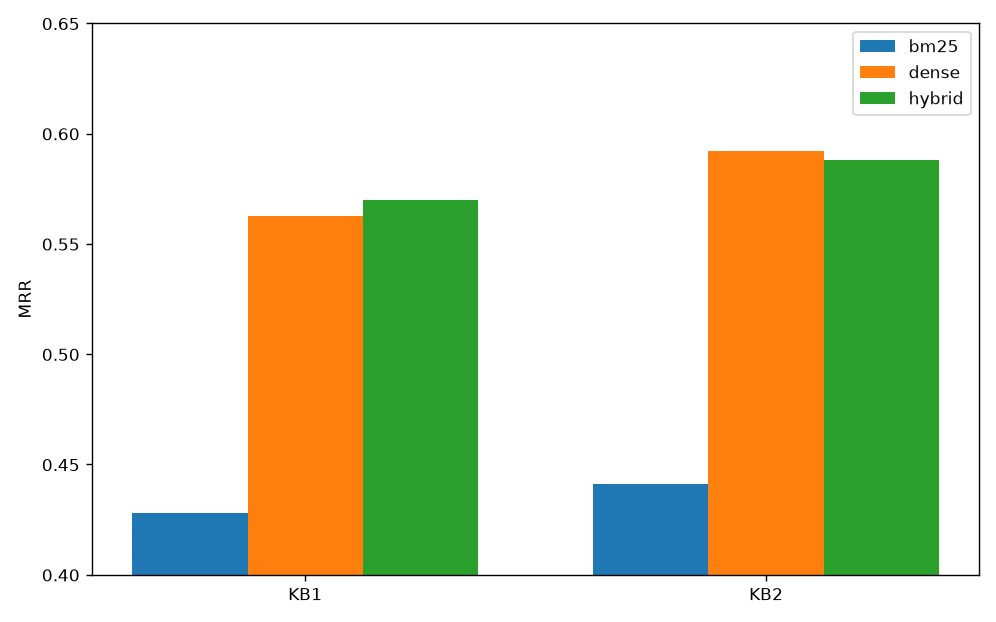
\includegraphics[width=\linewidth]{figures/overall_retrieval_mrr.png}
        \caption{MRR}
        \label{fig:overall_retrieval_mrr}
    \end{subfigure}

    \vspace{0.2cm}

    % Row 3
    \begin{subfigure}[t]{0.48\textwidth}
        \centering
        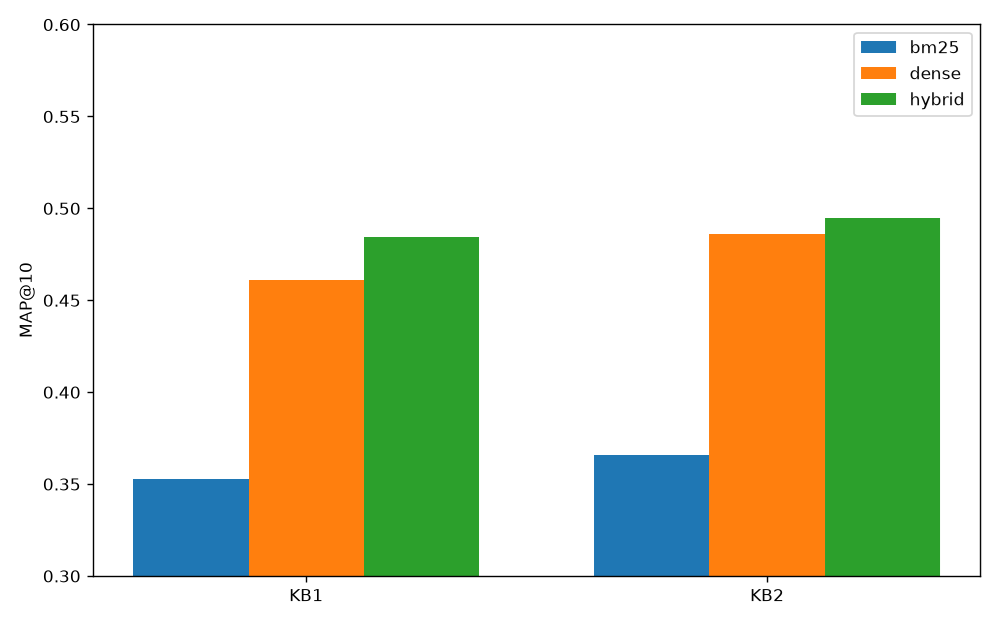
\includegraphics[width=\linewidth]{figures/overall_retrieval_map10.png}
        \caption{MAP@10}
        \label{fig:overall_retrieval_map10}
    \end{subfigure}
    \hfill
    \begin{subfigure}[t]{0.48\textwidth}
        \centering
        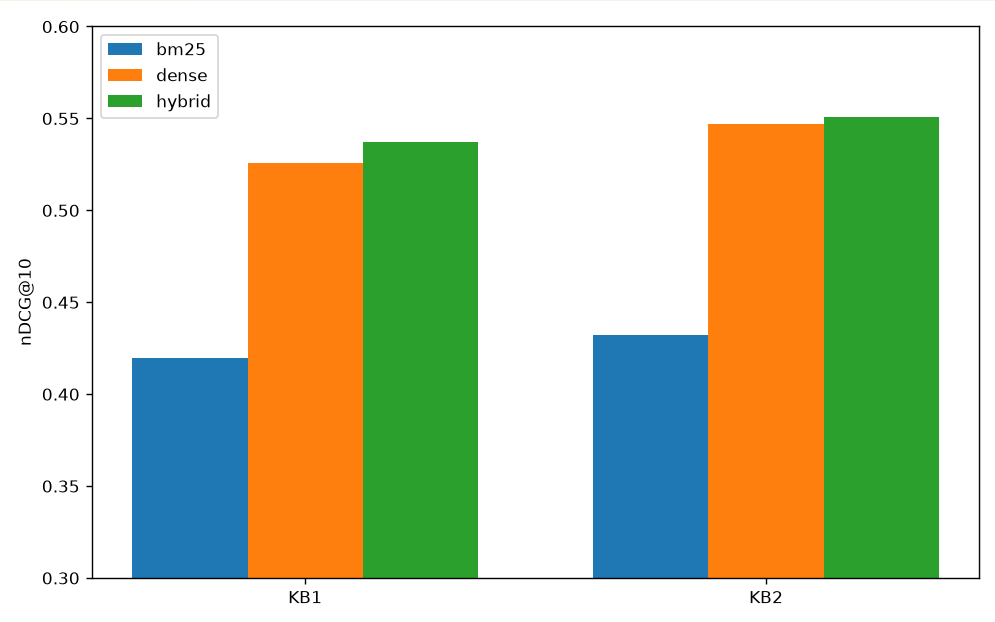
\includegraphics[width=\linewidth]{figures/overall_retrieval_ndcg10.png}
        \caption{nDCG@10}
        \label{fig:overall_retrieval_ndcg10}
    \end{subfigure}

    \caption{Overall comparison of BM25, dense, and hybrid retrieval performance across KB1 and KB2 using six evaluation metrics: Recall@10, Recall@20, Recall@50, MRR, MAP@10, and nDCG@10.}
    \label{fig:overall_retrieval_comparison}
\end{figure}

\begin{table}[htbp]
    \centering
    \caption{Overall retrieval performance of BM25, dense, and hybrid retrieval using KB1 and KB2}
    \label{tab:overall_retrieval_performance}

    \small
    \renewcommand{\arraystretch}{1.4}
    \setlength{\tabcolsep}{5pt}

    \begin{tabular}{l ccc ccc}
        \toprule
        & \multicolumn{3}{c}{\textbf{KB1}}
        & \multicolumn{3}{c}{\textbf{KB2}} \\
        \cmidrule(lr){2-4}
        \cmidrule(lr){5-7}

        \textbf{Metric} &
        \textbf{BM25} &
        \textbf{Dense} &
        \textbf{Hybrid} &
        \textbf{BM25} &
        \textbf{Dense} &
        \textbf{Hybrid} \\
        \midrule

        \textbf{Recall@10} &
        0.547 & \textbf{0.614} & 0.605 &
        0.557 & 0.619 & \textbf{0.620} \\

        \textbf{Recall@20} &
        0.625 & 0.660 & \textbf{0.680} &
        0.626 & 0.663 & \textbf{0.681} \\

        \textbf{Recall@50} &
        0.687 & 0.749 & \textbf{0.759} &
        0.679 & 0.753 & \textbf{0.769} \\

        \textbf{MRR} &
        0.428 & 0.563 & \textbf{0.570} &
        0.441 & \textbf{0.592} & 0.588 \\

        \textbf{MAP@10} &
        0.353 & 0.461 & \textbf{0.484} &
        0.366 & 0.486 & \textbf{0.495} \\

        \textbf{nDCG@10} &
        0.419 & 0.526 & \textbf{0.537} &
        0.432 & 0.547 & \textbf{0.551} \\

        \bottomrule
    \end{tabular}
\end{table}

For KB1, hybrid retrieval outperformed dense retrieval by approximately 1.9\% on average across the six evaluation metrics, achieving higher scores in five out of six metrics. Compared with BM25, hybrid retrieval demonstrated an average relative improvement of 21.4\%, outperforming it across all six metrics. Similarly, for KB2, hybrid retrieval outperformed dense retrieval by approximately 1.2\% on average across five out of six metrics, while achieving an average relative improvement of 21.5\% over BM25 across all six metrics.

Overall, these results suggest that the transition from KB1 to KB2 has only a limited effect on retrieval performance, since the relative differences between the retrieval methods remain almost unchanged across both knowledge base versions. In both cases, hybrid retrieval consistently performs best or close to best and provides a substantial advantage over BM25, while its improvement over dense retrieval remains relatively small. This indicates that the retrieval method has a stronger influence on retrieval quality than the choice between KB1 and KB2.
\subsection{Retrieval Performance for Common and Rare Battles}
In the second retrieval experiment, we investigated the performance of the retrieval algorithms on queries filtered by common and rare battles. The relative performance changed slightly. We noticed that for common battles, dense retrieval achieves the best results on five of the six evaluation metrics, while for rare-battle queries, hybrid retrieval outperformed dense retrieval across all six evaluation metrics, with an average relative improvement of approximately 13.1\%. The largest improvement was observed for Recall@50, where hybrid retrieval achieved a 21.8\% higher score. Table~\ref{tab:retrieval_common_rare} provides the corresponding metric values for both common- and rare-battle queries. Figure~\ref{fig:rarity_retrieval_comparison} additionally visualizes these results. Each bar chart demonstrates the results for one particular metric. For common battles, dense retrieval outperforms hybrid retrieval by around 3.9\% on average across all six metrics, with the largest improvement observed for Recall@10 at 6.2\%. Compared with BM25, dense retrieval improves the average score by approximately 34.8\%, with the largest improvements observed in MRR and MAP@10.

\begin{figure}[!htbp]
    \centering

    % Row 1: Recall@10 and Recall@20
    \begin{subfigure}[t]{0.48\textwidth}
        \centering
        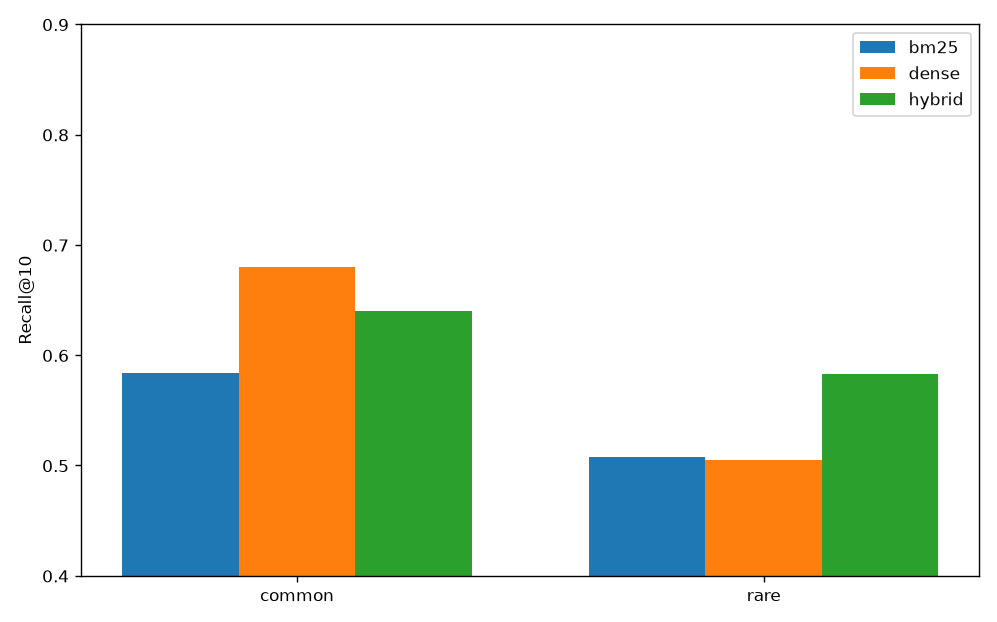
\includegraphics[width=\linewidth]{figures/rarity_retrieval_recall10.png}
        \caption{Recall@10}
        \label{fig:rarity_retrieval_recall10}
    \end{subfigure}
    \hfill
    \begin{subfigure}[t]{0.48\textwidth}
        \centering
        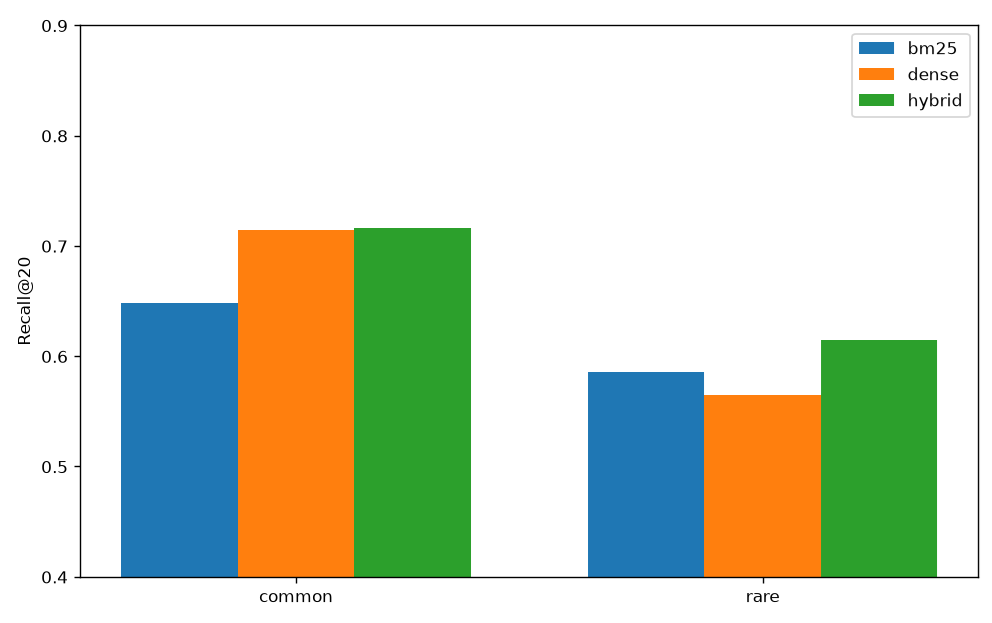
\includegraphics[width=\linewidth]{figures/rarity_retrieval_recall20.png}
        \caption{Recall@20}
        \label{fig:rarity_retrieval_recall20}
    \end{subfigure}

    \vspace{0.2cm}

    % Row 2: Recall@50 and MRR
    \begin{subfigure}[t]{0.48\textwidth}
        \centering
        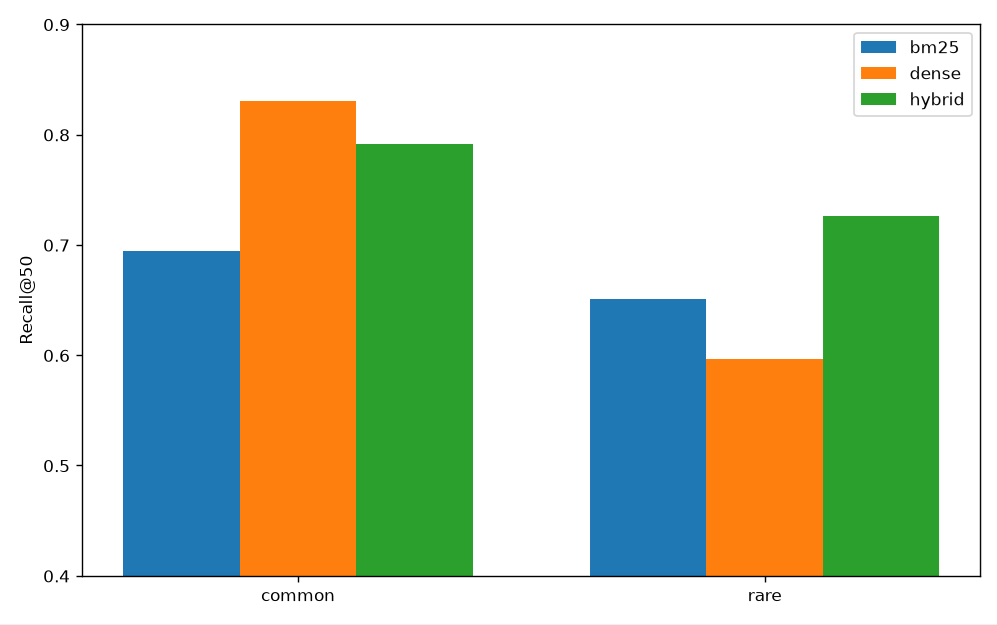
\includegraphics[width=\linewidth]{figures/rarity_retrieval_recall50.png}
        \caption{Recall@50}
        \label{fig:rarity_retrieval_recall50}
    \end{subfigure}
    \hfill
    \begin{subfigure}[t]{0.48\textwidth}
        \centering
        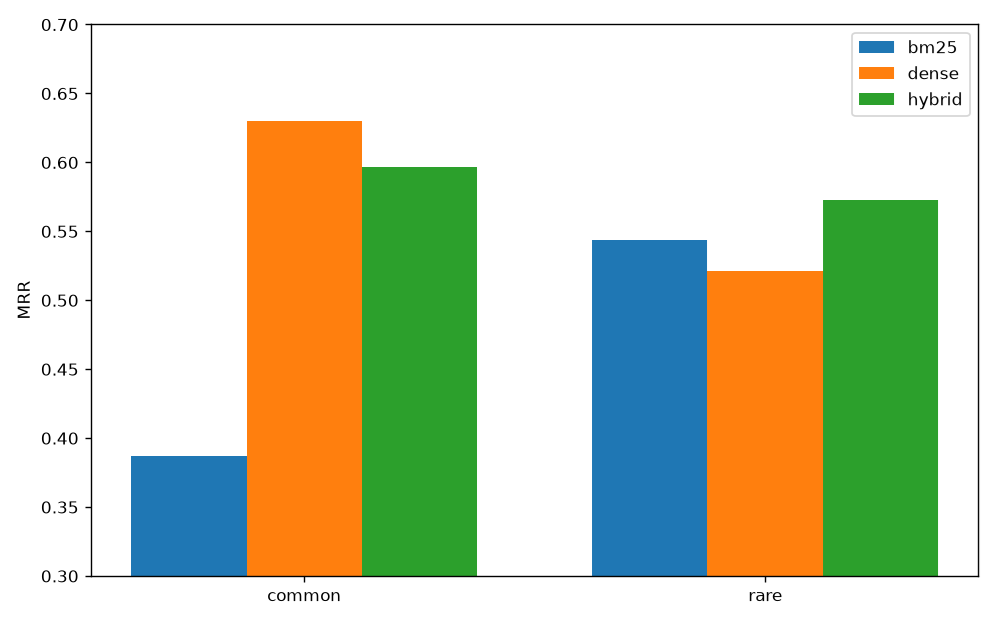
\includegraphics[width=\linewidth]{figures/rarity_retrieval_mrr.png}
        \caption{MRR}
        \label{fig:rarity_retrieval_mrr}
    \end{subfigure}

    \vspace{0.2cm}

    % Row 3: MAP@10 and nDCG@10
    \begin{subfigure}[t]{0.48\textwidth}
        \centering
        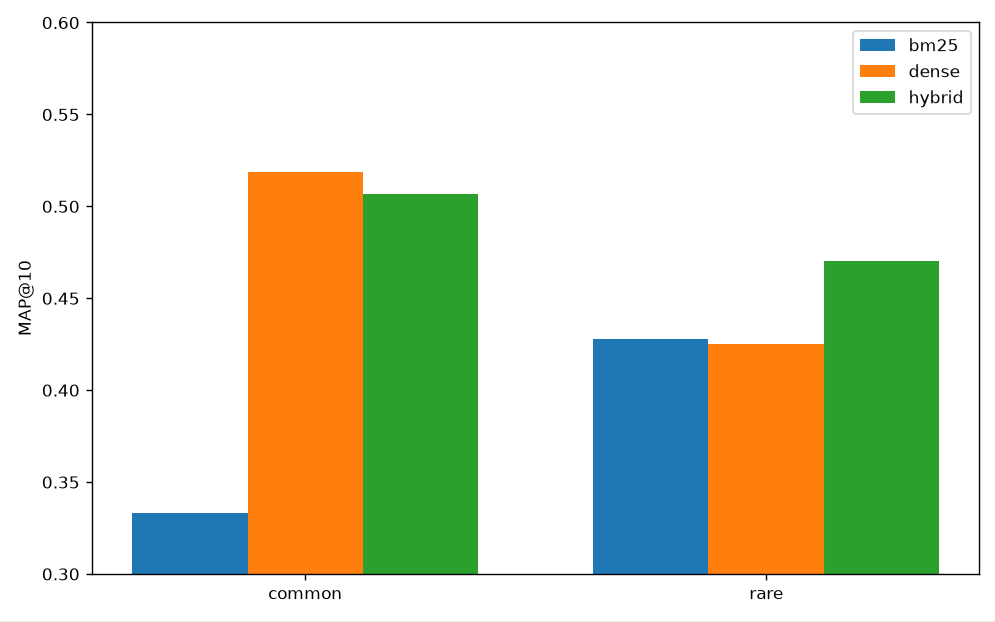
\includegraphics[width=\linewidth]{figures/rarity_retrieval_map10.png}
        \caption{MAP@10}
        \label{fig:rarity_retrieval_map10}
    \end{subfigure}
    \hfill
    \begin{subfigure}[t]{0.48\textwidth}
        \centering
        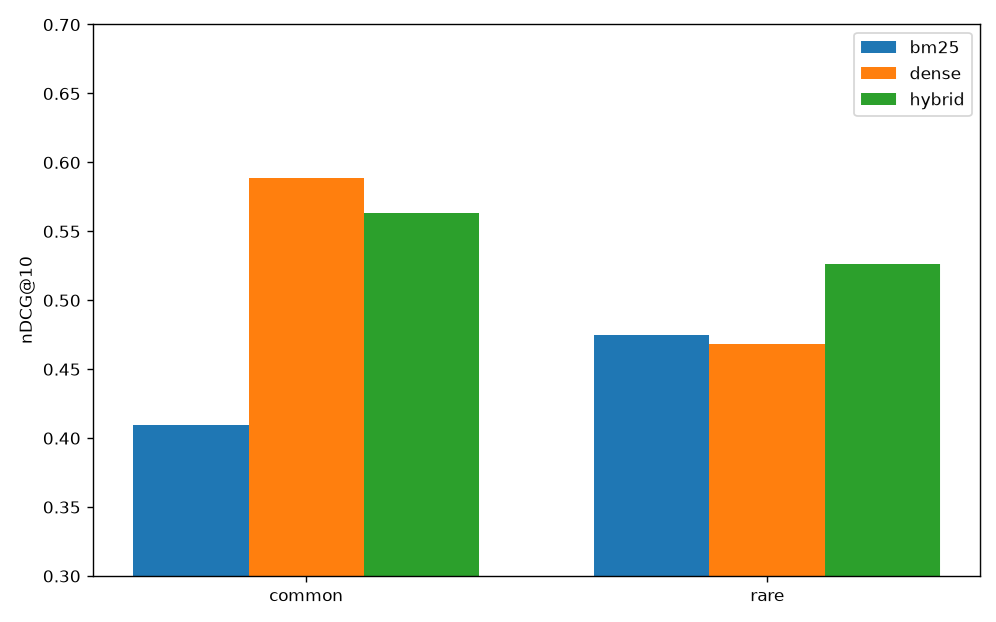
\includegraphics[width=\linewidth]{figures/rarity_retrieval_ndcg10.png}
        \caption{nDCG@10}
        \label{fig:rarity_retrieval_ndcg10}
    \end{subfigure}

    \caption{Comparison of BM25, dense, and hybrid retrieval performance for common and rare historical battle queries across six evaluation metrics: Recall@10, Recall@20, Recall@50, MRR, MAP@10, and nDCG@10.}
    \label{fig:rarity_retrieval_comparison}
\end{figure}

\begin{table}[htbp]
    \centering
    \caption{Retrieval performance of BM25, dense, and hybrid retrieval for common and rare battle queries}
    \label{tab:retrieval_common_rare}

    \small
    \renewcommand{\arraystretch}{1.4}
    \setlength{\tabcolsep}{5pt}

    \begin{tabular}{l ccc ccc}
        \toprule
        & \multicolumn{3}{c}{\textbf{Common}}
        & \multicolumn{3}{c}{\textbf{Rare}} \\
        \cmidrule(lr){2-4}
        \cmidrule(lr){5-7}

        \textbf{Metric} &
        \textbf{BM25} &
        \textbf{Dense} &
        \textbf{Hybrid} &
        \textbf{BM25} &
        \textbf{Dense} &
        \textbf{Hybrid} \\
        \midrule

        \textbf{Recall@10} &
        0.584 & \textbf{0.680} & 0.640 &
        0.508 & 0.505 & \textbf{0.583} \\

        \textbf{Recall@20} &
        0.648 & 0.715 & \textbf{0.716} &
        0.586 & 0.565 & \textbf{0.615} \\

        \textbf{Recall@50} &
        0.694 & \textbf{0.830} & 0.792 &
        0.651 & 0.596 & \textbf{0.727} \\

        \textbf{MRR} &
        0.387 & \textbf{0.630} & 0.596 &
        0.543 & 0.521 & \textbf{0.572} \\

        \textbf{MAP@10} &
        0.333 & \textbf{0.519} & 0.507 &
        0.428 & 0.425 & \textbf{0.470} \\

        \textbf{nDCG@10} &
        0.409 & \textbf{0.588} & 0.563 &
        0.475 & 0.468 & \textbf{0.526} \\

        \bottomrule
    \end{tabular}

    \par\vspace{4pt}
    \begin{minipage}{\linewidth}
        \footnotesize
        \textit{Note:} Bold values indicate the best-performing
        retrieval method for each metric within the corresponding
        query rarity group.
    \end{minipage}

\end{table}
One notable observation is the relatively low performance of BM25 for common battles. Although these battles are generally well known, lexical retrieval still depends on direct term overlap between the query and the JSON battle representation. We therefore decided to inspect several retrieval results in detail and found that semantically equivalent tactical descriptions can still use considerably different wording.

A representative example of this difference is query q048: \textit{Find a medieval battle where English longbows and defensive positioning combined to defeat French mounted and dismounted attacks.} The Battle of Agincourt strongly satisfies these conditions; however, BM25 ranked it only 27th, while dense retrieval placed it in the top three. The reason is that terms in the query such as \textit{defensive positioning}, \textit{mounted attacks}, and \textit{dismounted attacks} are expressed differently in the JSON battle representation, particularly through phrases such as \textit{defensive deployment behind stakes}, \textit{French cavalry charge}, \textit{infantry assault}, and \textit{French men-at-arms}. Dense retrieval was better able to capture these semantic associations. Table~\ref{tab:agincourt_query_wording} shows the different wording used in query q048 and the corresponding battle representation. This example illustrates how lexical retrieval can rank semantically similar battles differently because of differences in wording, while dense retrieval is better able to capture equivalent terminology.
\begin{table}[htbp]
    \centering
    \caption{Comparison of query wording and the structured representation of the Battle of Agincourt}
    \label{tab:agincourt_query_wording}

    \small
    \renewcommand{\arraystretch}{1.5}
    \setlength{\tabcolsep}{6pt}

    \begin{tabular}{
        >{\raggedright\arraybackslash}p{0.35\textwidth}
        >{\raggedright\arraybackslash}p{0.55\textwidth}
    }
        \toprule
        \textbf{Query wording} &
        \textbf{Agincourt representation} \\
        \midrule

        \texttt{longbows} &
        \texttt{longbow}, \texttt{longbowmen},
        \texttt{longbow volleys} \\
        \midrule

        \texttt{defensive positioning} &
        \texttt{defensive deployment behind stakes},
        \texttt{defensive position} \\
        \midrule

        \texttt{mounted attacks} &
        \texttt{French cavalry charge},
        \texttt{heavy cavalry} \\
        \midrule

        \texttt{dismounted attacks} &
        \texttt{French men-at-arms},
        \texttt{infantry assault},
        \texttt{advanced through mud} \\
        \midrule

        \texttt{attacks} &
        \texttt{charge}, \texttt{assault},
        \texttt{advance} \\

        \bottomrule
    \end{tabular}
\end{table}

Overall, these results suggest that the relative performance of the retrieval pipelines depends less on context rarity itself and more on how the query and the corresponding JSON battle representation are formulated. In particular, retrieval quality is strongly influenced by the amount of lexical overlap between the query and the battle record, as well as by how well their wording expresses the same underlying semantic concepts. Dense retrieval is therefore particularly useful when tactically similar information is described using different terminology. At the same time, hybrid retrieval achieves strong results for both common- and rare-battle queries by combining lexical and semantic relevance signals, and provides a substantial improvement especially for rare-battle queries.
\subsection{Retrieval Performance by Query Type}
In the next sub-experiment, we explored how different query types affect the performance of the retrieval methods. Table~\ref{tab:retrieval_query_types_1}, Table~\ref{tab:retrieval_query_types_2} and Table~\ref{tab:retrieval_similarity} shows clear differences across all seven query types. Temporal queries achieve the strongest overall results, with dense retrieval reaching the highest average score across the six metrics at approximately 0.890, compared with 0.802 for lexical retrieval and 0.868 for hybrid retrieval. Dense retrieval improves the average score over BM25 by about 11.1\% across the six metrics, while also achieving near-ceiling Recall values, including Recall@20 = 1.0 and Recall@50 = 1.0.
\begin{table}[H]
    \centering
    \caption{Retrieval performance across participant-related, spatial/terrain, and temporal query types}
    \label{tab:retrieval_query_types_1}

    \scriptsize
    \renewcommand{\arraystretch}{1.4}
    \setlength{\tabcolsep}{3pt}

    \begin{tabular}{l ccc ccc ccc}
        \toprule
        & \multicolumn{3}{c}{\textbf{Participant-related}}
        & \multicolumn{3}{c}{\textbf{Spatial / Terrain}}
        & \multicolumn{3}{c}{\textbf{Temporal}} \\
        \cmidrule(lr){2-4}
        \cmidrule(lr){5-7}
        \cmidrule(lr){8-10}

        \textbf{Metric} &
        \textbf{BM25} & \textbf{Dense} & \textbf{Hybrid} &
        \textbf{BM25} & \textbf{Dense} & \textbf{Hybrid} &
        \textbf{BM25} & \textbf{Dense} & \textbf{Hybrid} \\
        \midrule

        \textbf{Recall@10} &
        0.666 & 0.770 & \textbf{0.792} &
        \textbf{0.558} & 0.433 & 0.503 &
        0.800 & \textbf{0.950} & 0.913 \\

        \textbf{Recall@20} &
        0.811 & 0.826 & \textbf{0.874} &
        \textbf{0.571} & 0.471 & 0.548 &
        0.925 & \textbf{1.000} & 0.975 \\

        \textbf{Recall@50} &
        \textbf{0.930} & 0.841 & 0.926 &
        0.596 & 0.593 & \textbf{0.676} &
        \textbf{1.000} & \textbf{1.000} & \textbf{1.000} \\

        \textbf{MRR} &
        0.538 & \textbf{0.733} & 0.601 &
        0.364 & 0.521 & \textbf{0.637} &
        0.686 & \textbf{0.833} & 0.777 \\

        \textbf{MAP@10} &
        0.422 & \textbf{0.599} & 0.517 &
        0.291 & 0.315 & \textbf{0.472} &
        0.684 & 0.740 & \textbf{0.746} \\

        \textbf{nDCG@10} &
        0.514 & \textbf{0.686} & 0.621 &
        0.374 & 0.388 & \textbf{0.513} &
        0.716 & \textbf{0.819} & 0.796 \\

        \bottomrule
    \end{tabular}

    \par\vspace{4pt}
    \begin{minipage}{\linewidth}
        \footnotesize
        \textit{Note:} Bold values indicate the best-performing
        retrieval method for each metric within the corresponding
        query type.
    \end{minipage}

\end{table}
\begin{table}[H]
    \centering
    \caption{Retrieval performance of BM25, dense, and hybrid retrieval across outcome-related, narrative/tactical, and weapon/unit-related query types}
    \label{tab:retrieval_query_types_2}

    \scriptsize
    \renewcommand{\arraystretch}{1.4}
    \setlength{\tabcolsep}{3pt}

    \begin{tabular}{l ccc ccc ccc}
        \toprule
        & \multicolumn{3}{c}{\textbf{Outcome-related}}
        & \multicolumn{3}{c}{\textbf{Narrative / Tactical}}
        & \multicolumn{3}{c}{\textbf{Weapon / Unit-related}} \\
        \cmidrule(lr){2-4}
        \cmidrule(lr){5-7}
        \cmidrule(lr){8-10}

        \textbf{Metric} &
        \textbf{BM25} & \textbf{Dense} & \textbf{Hybrid} &
        \textbf{BM25} & \textbf{Dense} & \textbf{Hybrid} &
        \textbf{BM25} & \textbf{Dense} & \textbf{Hybrid} \\
        \midrule

        \textbf{Recall@10} &
        0.403 & 0.413 & \textbf{0.424} &
        0.373 & \textbf{0.548} & 0.469 &
        0.650 & 0.663 & \textbf{0.713} \\

        \textbf{Recall@20} &
        0.444 & 0.429 & \textbf{0.465} &
        0.388 & \textbf{0.578} & 0.560 &
        \textbf{0.746} & 0.729 & 0.738 \\

        \textbf{Recall@50} &
        0.493 & \textbf{0.612} & 0.499 &
        0.414 & \textbf{0.753} & 0.693 &
        0.788 & 0.750 & \textbf{0.842} \\

        \textbf{MRR} &
        0.179 & \textbf{0.375} & 0.356 &
        0.360 & \textbf{0.532} & 0.457 &
        0.544 & 0.624 & \textbf{0.735} \\

        \textbf{MAP@10} &
        0.163 & \textbf{0.343} & 0.311 &
        0.281 & \textbf{0.418} & 0.344 &
        0.428 & 0.546 & \textbf{0.643} \\

        \textbf{nDCG@10} &
        0.226 & \textbf{0.368} & 0.352 &
        0.319 & \textbf{0.477} & 0.404 &
        0.514 & 0.594 & \textbf{0.685} \\

        \bottomrule
    \end{tabular}

    \par\vspace{4pt}
    \begin{minipage}{\linewidth}
        \footnotesize
        \textit{Note:} Bold values indicate the best-performing
        retrieval method for each metric within the corresponding
        query type.
    \end{minipage}

\end{table}
\begin{table}[H]
    \centering
    \caption{Retrieval performance of BM25, dense, and hybrid retrieval for Similarity queries}
    \label{tab:retrieval_similarity}

    \small
    \renewcommand{\arraystretch}{1.4}
    \setlength{\tabcolsep}{12pt}

    \begin{tabular}{l ccc}
        \toprule
        & \multicolumn{3}{c}{\textbf{Similarity}} \\
        \cmidrule(lr){2-4}

        \textbf{Metric} &
        \textbf{BM25} &
        \textbf{Dense} &
        \textbf{Hybrid} \\
        \midrule

        \textbf{Recall@10} &
        0.050 & \textbf{0.307} & 0.203 \\

        \textbf{Recall@20} &
        0.190 & \textbf{0.390} & 0.303 \\

        \textbf{Recall@50} &
        0.363 & 0.455 & \textbf{0.530} \\

        \textbf{MRR} &
        0.046 & \textbf{0.204} & 0.133 \\

        \textbf{MAP@10} &
        0.010 & \textbf{0.122} & 0.055 \\

        \textbf{nDCG@10} &
        0.024 & \textbf{0.189} & 0.109 \\

        \bottomrule
    \end{tabular}

    \par\vspace{4pt}
    \begin{minipage}{0.75\textwidth}
        \footnotesize
        \textit{Note:} Bold values indicate the
        best-performing retrieval method for each metric.
    \end{minipage}

\end{table}
In contrast, Similarity queries remain the most difficult for lexical retrieval. BM25 achieves particularly low scores, with Recall@10 = 0.05, MRR $\approx$ 0.046, and MAP@10 = 0.01. Dense retrieval, on the other hand, reaches 0.307, 0.204, and 0.122 for these metrics, respectively. Across all six metrics, dense retrieval improves the average score from approximately 0.114 for BM25 to 0.278, corresponding to a relative improvement of about 143.9\%. This provides strong evidence that semantic matching is especially helpful for Similarity queries, where lexical overlap may be insufficient.

We observed a different pattern for Spatial/Terrain queries. Here, BM25 and dense retrieval achieve similar average scores across the six metrics, at approximately 0.459 and 0.453, respectively, while hybrid retrieval achieves a higher average score of approximately 0.558. This corresponds to a 23.1\% relative improvement over dense retrieval. The largest gains are observed in the ranking-sensitive metrics: MRR increases from 0.521 for dense retrieval to 0.637 for hybrid retrieval, MAP@10 increases from 0.315 to 0.472, and nDCG@10 increases from 0.388 to 0.513, showing a similar trend.

Overall, the hybrid retrieval strategy provides a very consistent improvement over BM25, achieving higher scores in 37 of 42 metric comparisons and higher average performance across all six metrics for all seven query types. However, its advantage over dense retrieval is more selective. Hybrid retrieval achieves better results in 19 of 42 metric comparisons and a higher average score in only two query types: Spatial/Terrain and Weapon/Unit-related. This suggests that although hybrid retrieval provides a robust improvement over purely lexical retrieval, its benefit over dense retrieval depends more strongly on the characteristics of the query type.
\section{Oracle-context Generation Results}
In Chapter 4.2, we introduced the Oracle-context generation experiment, which is designed to evaluate the generation step in isolation, without the influence of retrieval quality. For each query, the model is provided with a predefined set of candidate battles to choose from, containing both battles from the gold set and hard negatives. We divided the Oracle-context generation experiment into three parts. First, we evaluated overall generation performance across the complete query set by comparing the baseline LLM, raw-text-augmented LLM, and JSON-augmented LLM, while also assessing the JSON-augmented results obtained using KB1 and KB2 separately. In the second sub-experiment, we analyzed generation performance separately for queries involving common and rare battles. Finally, we compared generation performance across the different query types. We used four main metrics for the analysis: precision, recall, F1, and exact match. In addition, we recorded the number of parse errors and run errors.
\subsection{Overall Generation Performance}
We summarize the Oracle-context generation results in Table~\ref{tab:oracle_overall_performance} and additionally visualize them in Figure~\ref{fig:overall_oracle_comparison}. The comparison between KB1 and KB2 shows that the verification and regeneration pipeline used to construct KB2 did not lead to a substantial improvement over KB1. As shown in Table 5.2.1.1, KB2 achieved almost identical recall and the same exact-match score as KB1, while precision and F1 were slightly lower. The bar chart further illustrates the small differences between the two JSON-augmented configurations.

\begin{figure}[!htbp]
    \centering

    % Row 1: Precision and Recall
    \begin{subfigure}[t]{0.40\textwidth}
        \centering
        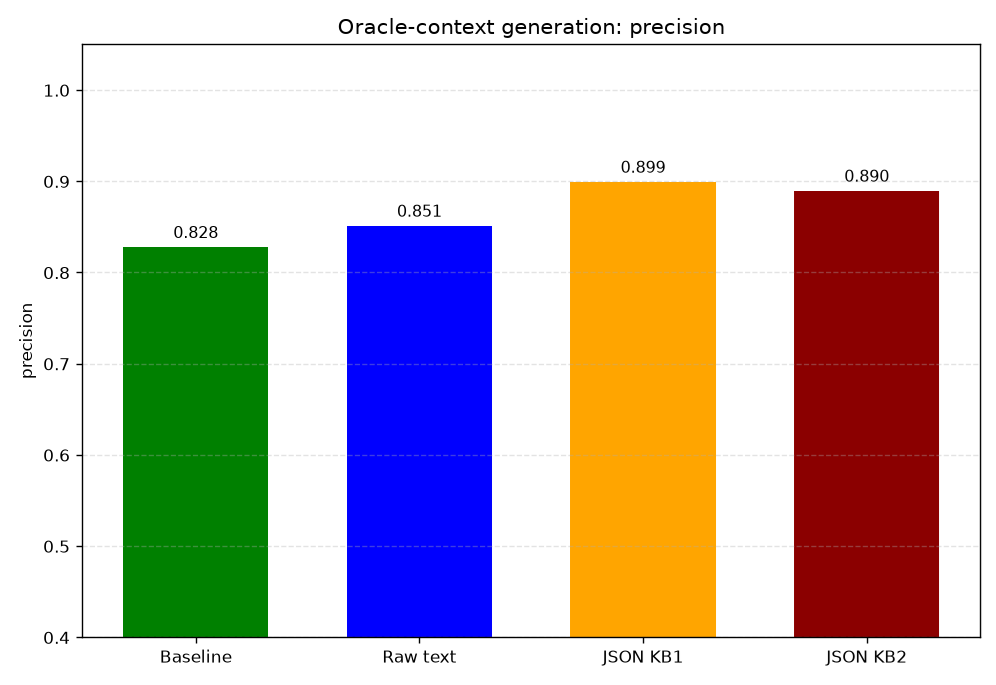
\includegraphics[width=\linewidth]{figures/overall_oracle_precision.png}
        \caption{Precision}
        \label{fig:overall_oracle_precision}
    \end{subfigure}
    \hfill
    \begin{subfigure}[t]{0.40\textwidth}
        \centering
        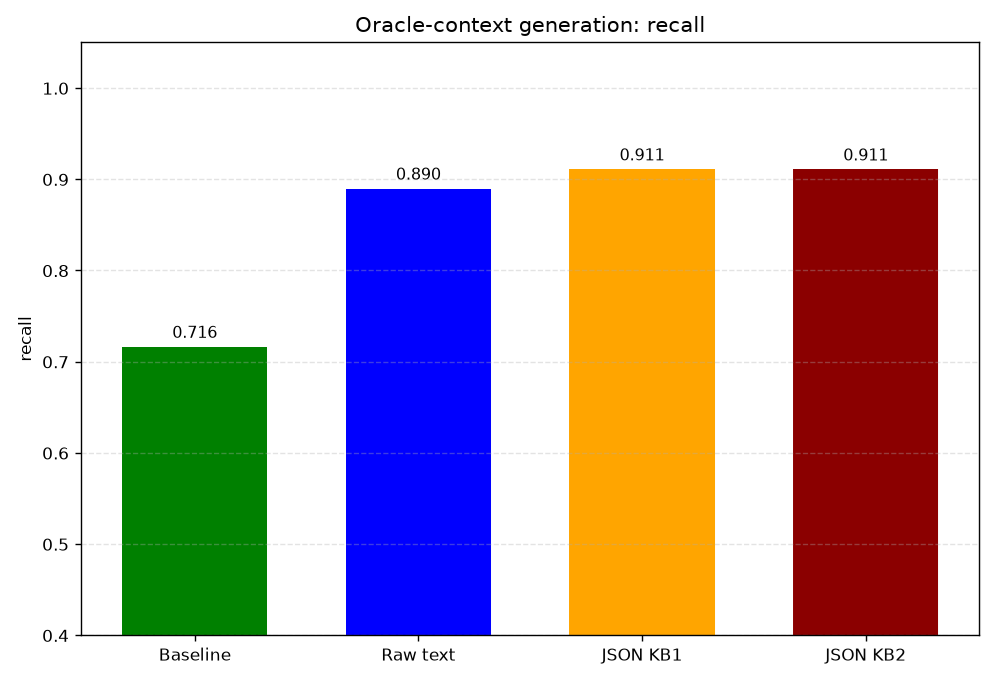
\includegraphics[width=\linewidth]{figures/overall_oracle_recall.png}
        \caption{Recall}
        \label{fig:overall_oracle_recall}
    \end{subfigure}

    \vspace{0.2cm}

    % Row 2: F1 and Exact Match
    \begin{subfigure}[t]{0.40\textwidth}
        \centering
        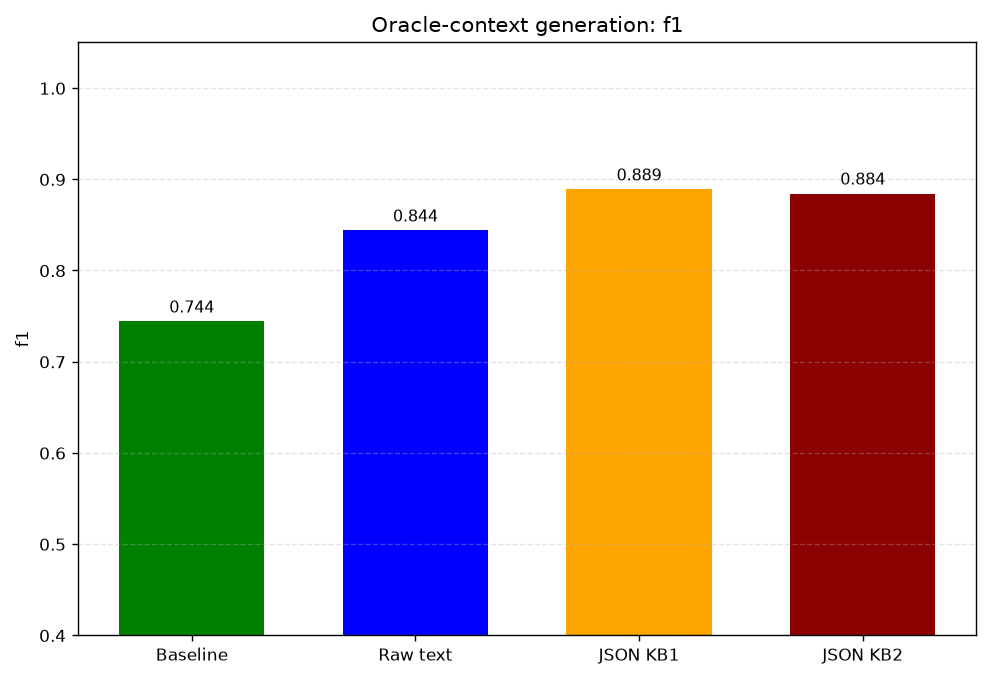
\includegraphics[width=\linewidth]{figures/overall_oracle_f1.png}
        \caption{F1 Score}
        \label{fig:overall_oracle_f1}
    \end{subfigure}
    \hfill
    \begin{subfigure}[t]{0.40\textwidth}
        \centering
        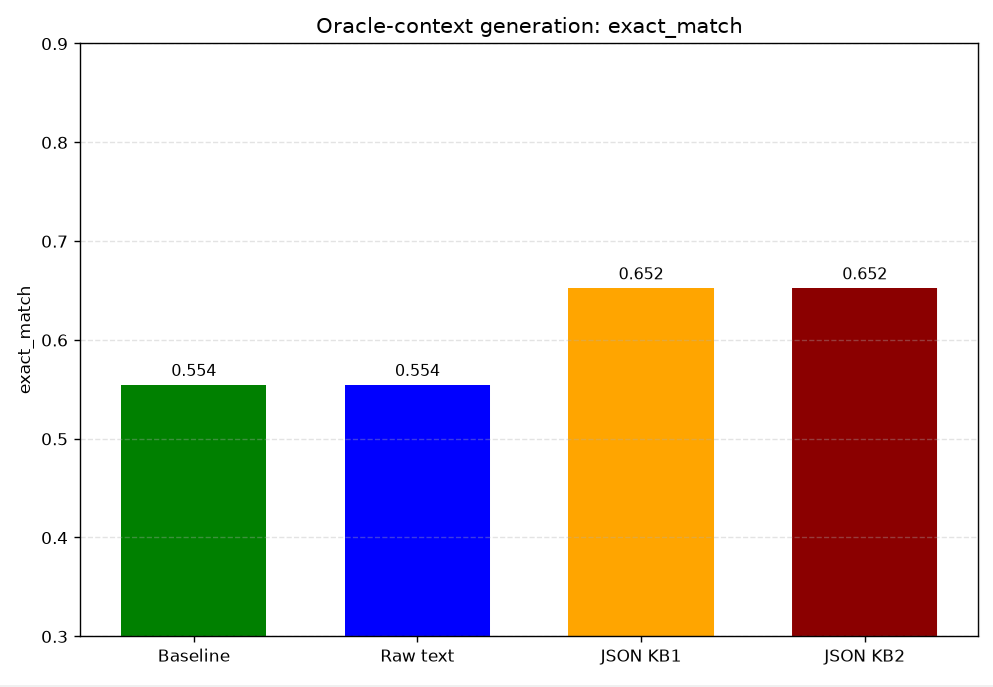
\includegraphics[width=\linewidth]{figures/overall_oracle_exact_match.png}
        \caption{Exact Match}
        \label{fig:overall_oracle_exact_match}
    \end{subfigure}

    \caption{Overall performance comparison of the baseline, raw-text, JSON KB1, and JSON KB2 configurations in the oracle-context generation experiment across four evaluation metrics: Precision, Recall, F1, and Exact Match.}
    \label{fig:overall_oracle_comparison}
\end{figure}

\begin{table}[H]
    \centering
    \caption{Overall Oracle-context generation performance across baseline, raw-text-augmented, JSON KB1, and JSON KB2 configurations}
    \label{tab:oracle_overall_performance}

    \small
    \renewcommand{\arraystretch}{1.4}
    \setlength{\tabcolsep}{10pt}

    \begin{tabular}{l cccc}
        \toprule
        \textbf{Metric} &
        \textbf{Baseline} &
        \textbf{Raw-text} &
        \textbf{JSON KB1} &
        \textbf{JSON KB2} \\
        \midrule

        \textbf{Precision} &
        0.828 & 0.851 & \textbf{0.899} & 0.890 \\

        \textbf{Recall} &
        0.716 & 0.890 & \textbf{0.911} & \textbf{0.911} \\

        \textbf{F1} &
        0.744 & 0.844 & \textbf{0.889} & 0.884 \\

        \textbf{Exact Match} &
        0.554 & 0.554 & \textbf{0.652} & \textbf{0.652} \\

        \bottomrule
    \end{tabular}

    \par\vspace{4pt}
    \begin{minipage}{0.9\textwidth}
        \footnotesize
        \textit{Note:} Bold values indicate the
        best-performing configuration for each metric.
    \end{minipage}

\end{table}
In contrast, both JSON-augmented configurations clearly outperform the baseline LLM and the raw-text-augmented model across all four evaluation metrics. When using KB1, precision increased from 0.828 to 0.899 compared with the baseline LLM, corresponding to an improvement of 8.6\%. Recall, F1, and exact match also improved considerably, by 27.2\%, 19.5\%, and 17.7\%, respectively. The JSON-augmented models also perform slightly better than the raw-text-augmented model. Compared with raw-text augmentation, KB1 increased precision from 0.851 to 0.899, recall from 0.890 to 0.911, and exact match from 0.554 to 0.652, corresponding to improvements of 5.7\%, 2.4\%, and 17.7\%, respectively. On average across the four evaluation metrics, the KB1 JSON-augmented model achieved approximately 17.9\% higher performance than the baseline LLM and 6.8\% higher performance than the raw-text-augmented model. These results indicate an advantage of the structured battle representation in the controlled Oracle-context experiment.
\subsection{Generation Performance for Common and Rare Battles}
In this sub-experiment, we examine model performance in the Oracle-context setting separately for common- and rare-battle queries. Table~\ref{tab:oracle_common_rare} compares
Oracle-context generation performance across
common and rare battle queries. shows the metric scores for all four model configurations, while Figure~\ref{fig:rarity_oracle_comparison} visualizes precision, recall, F1, and exact match.

\begin{figure}[!htbp]
    \centering

    % Row 1: Precision and Recall
    \begin{subfigure}[t]{0.48\textwidth}
        \centering
        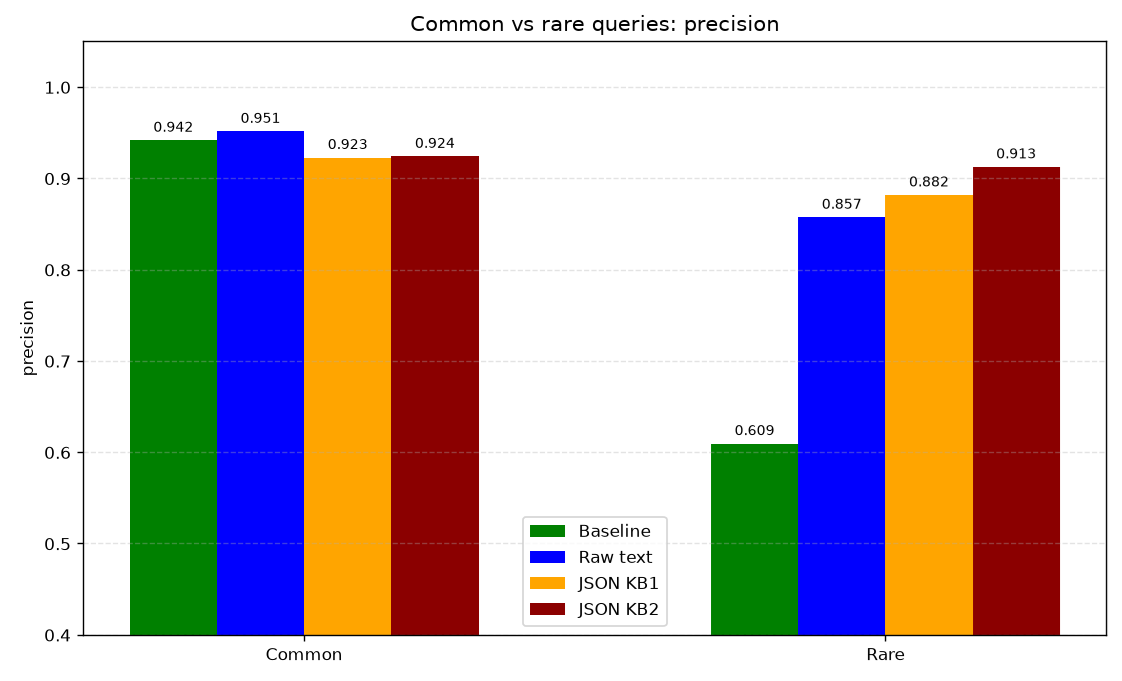
\includegraphics[width=\linewidth]{figures/rarity_oracle_precision.png}
        \caption{Precision}
        \label{fig:rarity_oracle_precision}
    \end{subfigure}
    \hfill
    \begin{subfigure}[t]{0.48\textwidth}
        \centering
        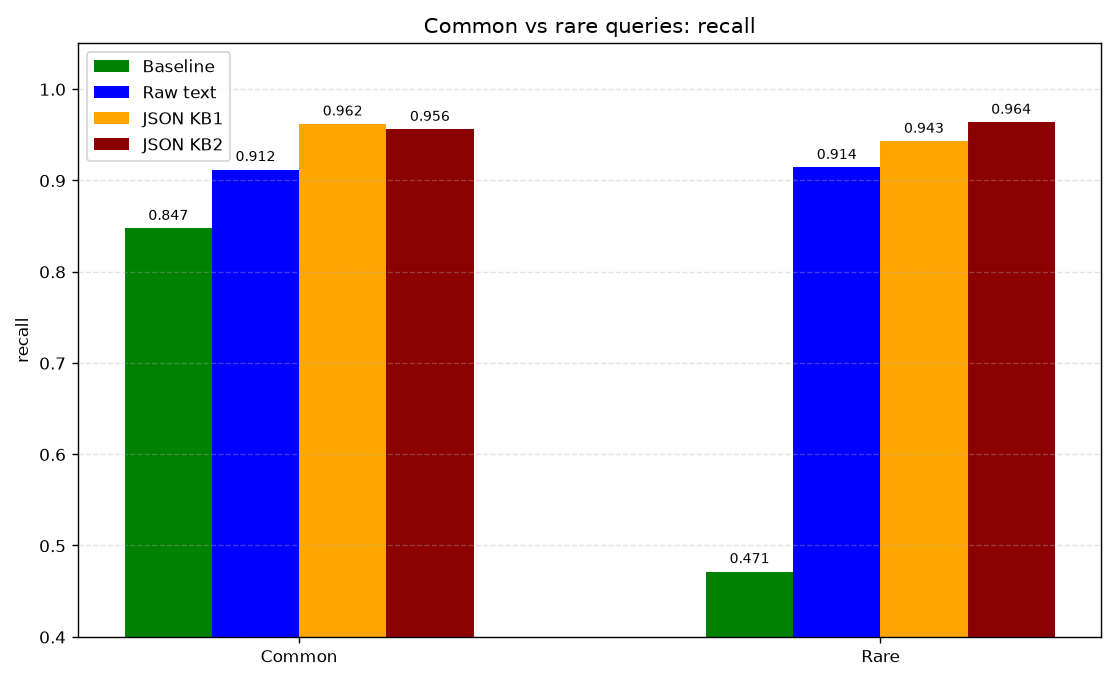
\includegraphics[width=\linewidth]{figures/rarity_oracle_recall.png}
        \caption{Recall}
        \label{fig:rarity_oracle_recall}
    \end{subfigure}

    \vspace{0.2cm}

    % Row 2: F1 and Exact Match
    \begin{subfigure}[t]{0.48\textwidth}
        \centering
        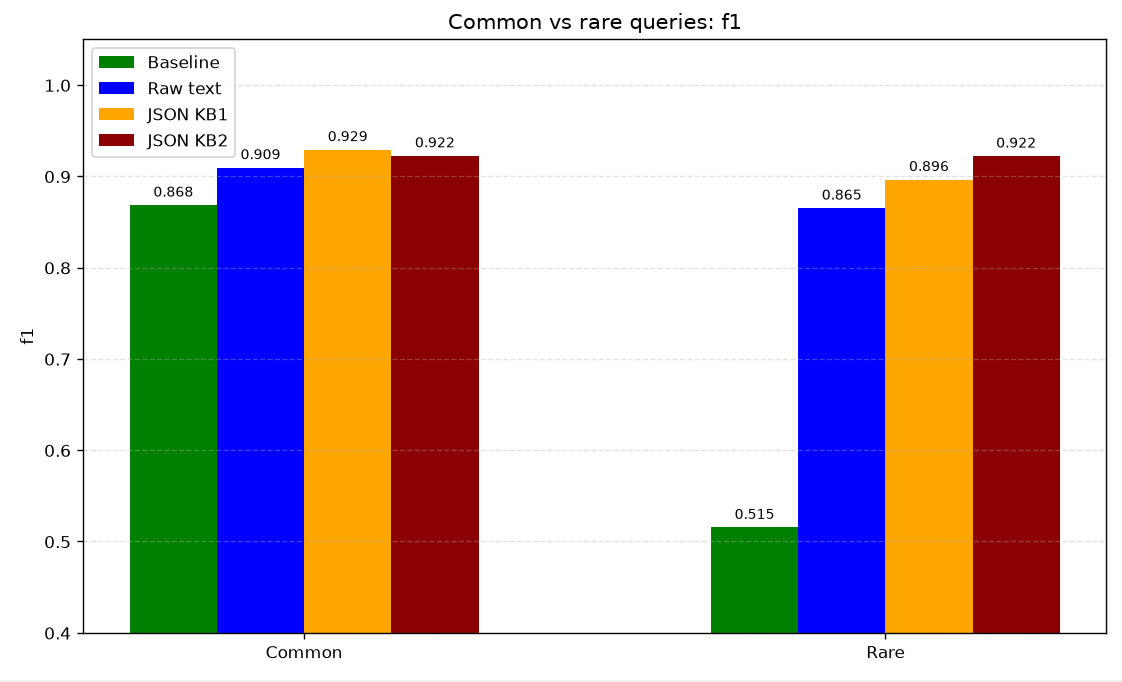
\includegraphics[width=\linewidth]{figures/rarity_oracle_f1.png}
        \caption{F1 Score}
        \label{fig:rarity_oracle_f1}
    \end{subfigure}
    \hfill
    \begin{subfigure}[t]{0.48\textwidth}
        \centering
        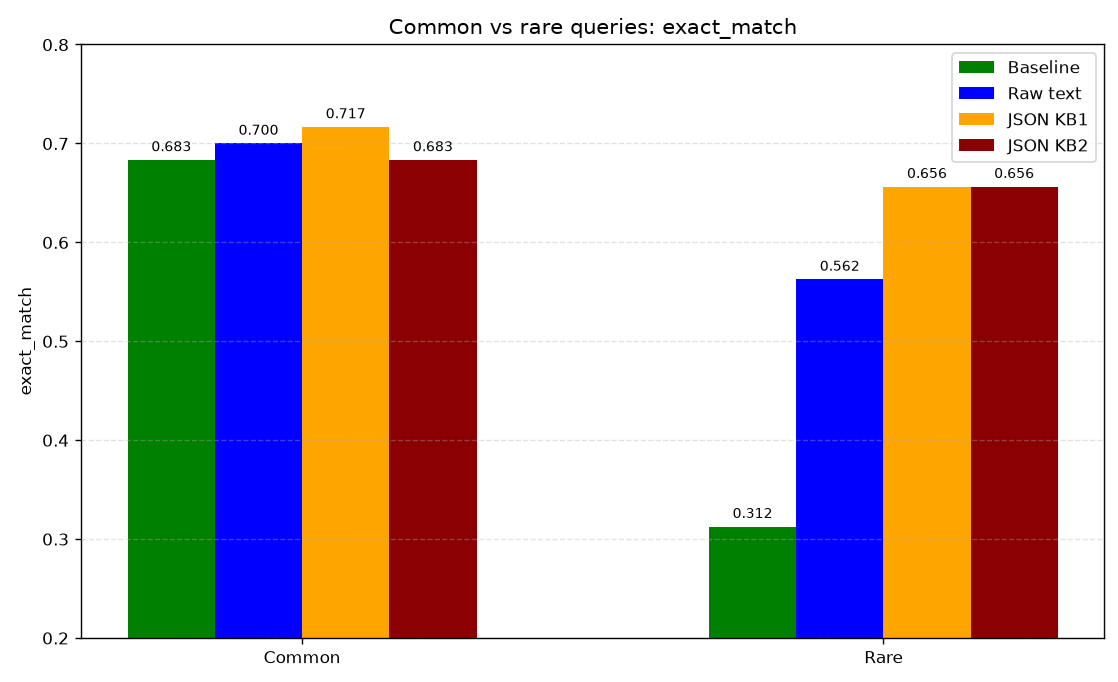
\includegraphics[width=\linewidth]{figures/rarity_oracle_exact_match.png}
        \caption{Exact Match}
        \label{fig:rarity_oracle_exact_match}
    \end{subfigure}

    \caption{Comparison of baseline, raw-text, JSON KB1, and JSON KB2 performance on common and rare historical battle queries in the oracle-context generation experiment, evaluated using Precision, Recall, F1, and Exact Match.}
    \label{fig:rarity_oracle_comparison}
\end{figure}

\begin{table}[H]
    \centering
    \caption{Oracle-context generation performance for common and rare battle queries across baseline, raw-text-augmented, JSON KB1, and JSON KB2 configurations}
    \label{tab:oracle_common_rare}

    \scriptsize
    \renewcommand{\arraystretch}{1.4}
    \setlength{\tabcolsep}{4pt}

    \begin{tabular}{l cccc cccc}
        \toprule
        & \multicolumn{4}{c}{\textbf{Common}}
        & \multicolumn{4}{c}{\textbf{Rare}} \\
        \cmidrule(lr){2-5}
        \cmidrule(lr){6-9}

        \textbf{Metric} &
        \textbf{Baseline} &
        \textbf{Raw-text} &
        \textbf{JSON KB1} &
        \textbf{JSON KB2} &
        \textbf{Baseline} &
        \textbf{Raw-text} &
        \textbf{JSON KB1} &
        \textbf{JSON KB2} \\
        \midrule

        \textbf{Precision} &
        0.942 & \textbf{0.951} & 0.923 & 0.924 &
        0.609 & 0.857 & 0.882 & \textbf{0.913} \\

        \textbf{Recall} &
        0.847 & 0.912 & \textbf{0.962} & 0.956 &
        0.471 & 0.914 & 0.943 & \textbf{0.964} \\

        \textbf{F1} &
        0.868 & 0.909 & \textbf{0.929} & 0.922 &
        0.515 & 0.865 & 0.896 & \textbf{0.922} \\

        \textbf{Exact Match} &
        0.683 & 0.700 & \textbf{0.717} & 0.683 &
        0.313 & 0.563 & \textbf{0.656} & \textbf{0.656} \\

        \bottomrule
    \end{tabular}

    \par\vspace{4pt}
    \begin{minipage}{\linewidth}
        \footnotesize
        \textit{Note:} Bold values indicate the
        best-performing configuration for each metric
        within the corresponding query rarity group.
    \end{minipage}

\end{table}
For common-battle queries, the baseline LLM achieves relatively strong results, with an average score of 0.835 across the four metrics. The raw-text-augmented model achieves a similar average score of 0.868, with improvements of 7.6\% in recall, 0.96\% in precision, and 2.49\% in exact match. The KB2 JSON-augmented model reaches an average score of 0.871, which is the highest among the three main model configurations, mainly due to achieving the highest recall of 0.956. Compared with the baseline, the JSON-augmented model improves recall by approximately 12.8\% and F1 by 6.2\%, while precision is slightly lower and exact match remains unchanged. These results illustrate that context augmentation provides only a moderate advantage for common-battle queries.

A substantially different pattern was observed for rare-battle queries. Here, the baseline LLM performs considerably worse, achieving a precision of 0.609, recall of 0.471, and exact match of 0.313. In contrast, the KB2 JSON-augmented model outperforms the baseline LLM by an average of approximately 81.1\% across all four evaluation metrics, achieving precision = 0.913, recall = 0.964, and exact match = 0.656. This corresponds to relative improvements of 49.7\% in precision and 104.4\% in recall. The raw-text-augmented model also achieves a substantial average relative improvement of approximately 67.7\% over the baseline LLM across the four metrics, while the JSON-augmented configuration remains the strongest overall.

Overall, these results suggest that external context containing battle representations provides only a limited advantage for common-battle queries, where the baseline LLM already performs well. However, it becomes much more beneficial for rare-battle queries, where structured JSON battle representations considerably improve the model’s ability to identify relevant battles, at least in the Oracle-context generation setting.

One representative example for JSON-augmented model advantage was observed for the query q089 \textit{From the provided battle set, identify battles where armoured trains directly influenced the tactical outcome by providing decisive fire support, disabling an opposing train, or causing enemy troops to abandon a key position.}. As Table~\ref{tab:oracle_battle_example} shows, the baseline LLM failed to identify both golden battles, the Battle of Motovylivka and the Battle of Vapniarka. Instead it selected two battles belonging to closed-set negatives such as Battle of Antrea and the Battle of Vilppula. This resulted in scores 0.0 for all 4 metrics. 
\begin{table}[H]
    \centering
    \caption{Oracle-context generation results for the Motovylivka and Vapniarka battle query}
    \label{tab:oracle_battle_example}

    \small
    \renewcommand{\arraystretch}{1.5}
    \setlength{\tabcolsep}{4pt}

    \begin{tabular}{
        >{\raggedright\arraybackslash}p{0.15\textwidth}
        >{\raggedright\arraybackslash}p{0.20\textwidth}
        c c c c c
    }
        \toprule
        \textbf{Configuration} &
        \textbf{Selected battles} &
        \textbf{Gold battles found} &
        \textbf{Precision} &
        \textbf{Recall} &
        \textbf{F1} &
        \textbf{Exact Match} \\
        \midrule

        Baseline LLM &
        Antrea; Vilppula &
        0/2 &
        0.000 &
        0.000 &
        0.000 &
        No \\
        \midrule

        JSON KB1 &
        Motovylivka; Vapniarka &
        2/2 &
        \textbf{1.000} &
        \textbf{1.000} &
        \textbf{1.000} &
        \textbf{Yes} \\
        \midrule

        JSON KB2 &
        Motovylivka; Vapniarka &
        2/2 &
        \textbf{1.000} &
        \textbf{1.000} &
        \textbf{1.000} &
        \textbf{Yes} \\

        \bottomrule
    \end{tabular}
\end{table}
This baseline-model failure is particularly interesting because it illustrates the problem of underrepresented knowledge about rare battles. The Battle of Motovylivka and the Battle of Vapniarka are relatively obscure engagements associated with the Ukrainian conflicts of 1918–1919. The Battle of Motovylivka was fought on 18 November 1918 between the Directorate of Ukraine and the Ukrainian State during the Ukrainian Civil War. Contemporary summaries, including our battle representation derived from the corresponding Wikipedia article, explicitly state that both sides employed armoured trains and that a Directorate armoured train disabled the opposing Hetman train \citep{wikipedia2026motovilivka}. The Battle of Vapniarka was fought during the Ukrainian–Soviet War in July 1919 around the strategically important Vapniarka railway station. Ukrainian forces used an improvised armoured train consisting of a cannon mounted on a railway platform, which contributed to panic and withdrawal among the Bolshevik forces \citep{wikipedia2026vapniarka}. Table~\ref{tab:oracle_json_evidence} illustrates the corresponding evidence stored in our local battle representations, which directly supported the JSON-augmented LLM in identifying these gold battles.
\begin{table}[H]
    \centering
    \caption{Evidence supporting the identification of gold-standard battles in JSON representations}
    \label{tab:oracle_json_evidence}

    \small
    \renewcommand{\arraystretch}{1.5}
    \setlength{\tabcolsep}{6pt}

    \begin{tabular}{
        >{\raggedright\arraybackslash}p{0.27\textwidth}
        >{\raggedright\arraybackslash}p{0.63\textwidth}
    }
        \toprule
        \textbf{Gold battle} &
        \textbf{Evidence available in JSON} \\
        \midrule

        \textbf{Battle of Motovylivka} &
        Directorate armoured train disabled the opposing
        Hetman armoured train with an artillery hit,
        forcing it to withdraw. \\
        \midrule

        \textbf{Battle of Vapniarka} &
        Improvised armoured train with a cannon supported
        the attack and contributed to the Bolshevik
        withdrawal from Vapniarka. \\

        \bottomrule
    \end{tabular}
\end{table}
In this example, the baseline model still produced plausible explanations for other candidate battles, but it lacked sufficient knowledge to identify the correct engagements. In contrast, the JSON-augmented model selected both gold battles and achieved perfect scores across all four evaluation metrics.
\section{End-to-End RAG Evaluation Results}
As previously discussed in Chapter 4.4, the goal of the final experiment is to evaluate the complete RAG pipeline, including both the retrieval and generation steps, and to compare the augmented models with the baseline LLM. In this setting, a predefined candidate set of battles is not provided. The baseline LLM receives only the query, while the augmented LLMs receive the top-$k$ battle instances retrieved by the hybrid retrieval pipeline. In the first sub-experiment, we evaluate all three model configurations across the complete query set, excluding the Similarity query type. Additionally, we test the JSON-augmented model using different numbers of retrieved battles, with \(k = 5, 10, 20,\) and \(30\), while the raw-text-augmented model is evaluated with \(k = 5, 10,\) and \(20\). In the two subsequent sub-experiments, we again evaluate the models separately for common- and rare-battle queries and across different query types. Unlike in the Oracle-context generation setting, we additionally apply faithfulness and context relevance metrics to evaluate the quality of the retrieved context.
\subsection{Overall Performance and Error Analysis}
The overall end-to-end RAG results across all 92 queries show that the JSON-augmented configuration performs similarly to the baseline LLM in terms of precision and exact-match accuracy, while achieving higher recall across the tested top-\(k\) settings. Table~\ref{tab:e2e_overall_performance} and Figure~\ref{fig:overall_e2e_comparison} show the metric results for all three model configurations across different top-\(k\) settings. The highest precision for the JSON-augmented model was achieved at \(k=10\), where precision increased to 0.499 compared with 0.467 for the baseline LLM, corresponding to an improvement of approximately 7.0\%. Compared with raw-text augmentation at the same context size, the JSON-augmented model achieved a 5.7\% higher precision.

\begin{figure}[!htbp]
    \centering

    % Row 1: Precision and Recall
    \begin{subfigure}[t]{0.48\textwidth}
        \centering
        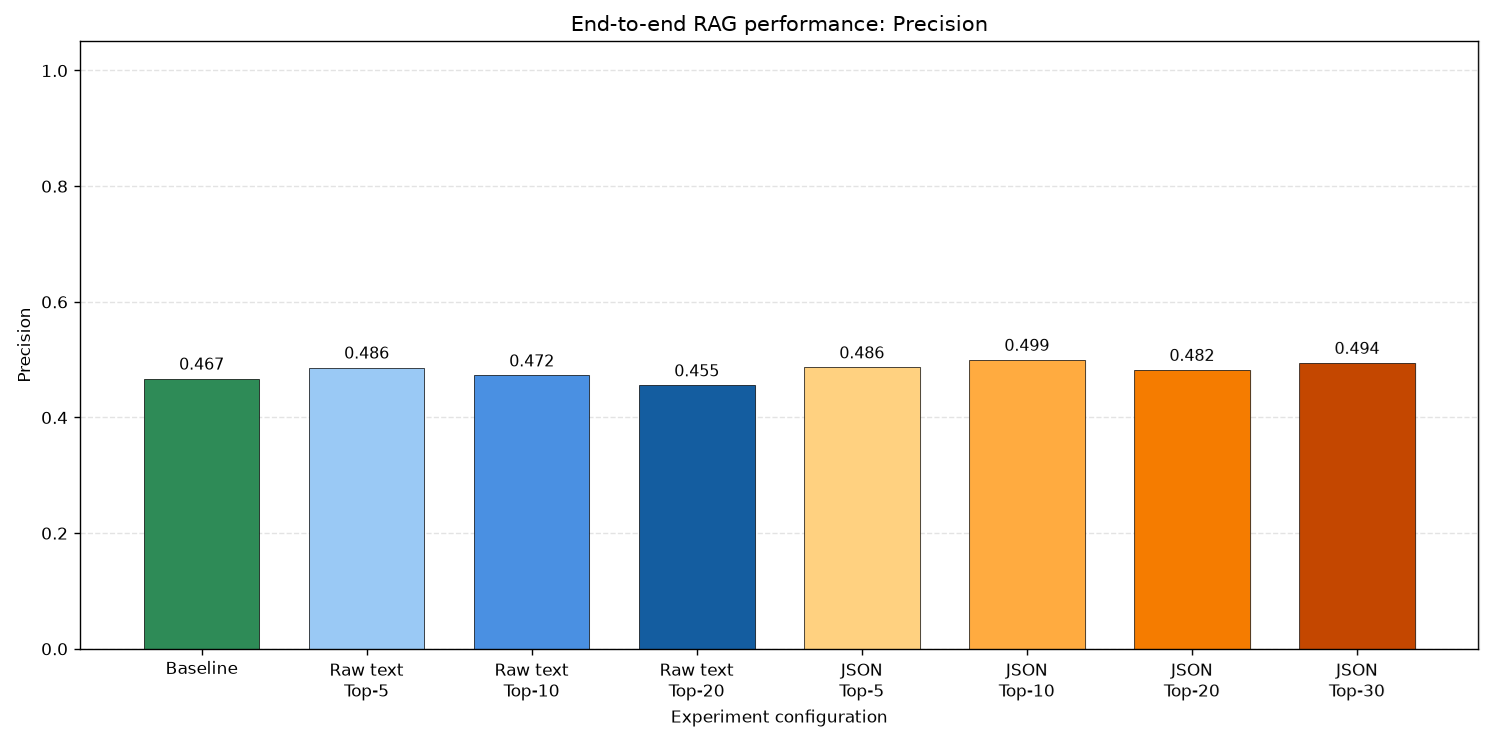
\includegraphics[width=\linewidth]{figures/overall_e2e_precision.png}
        \caption{Precision}
        \label{fig:overall_e2e_precision}
    \end{subfigure}
    \hfill
    \begin{subfigure}[t]{0.48\textwidth}
        \centering
        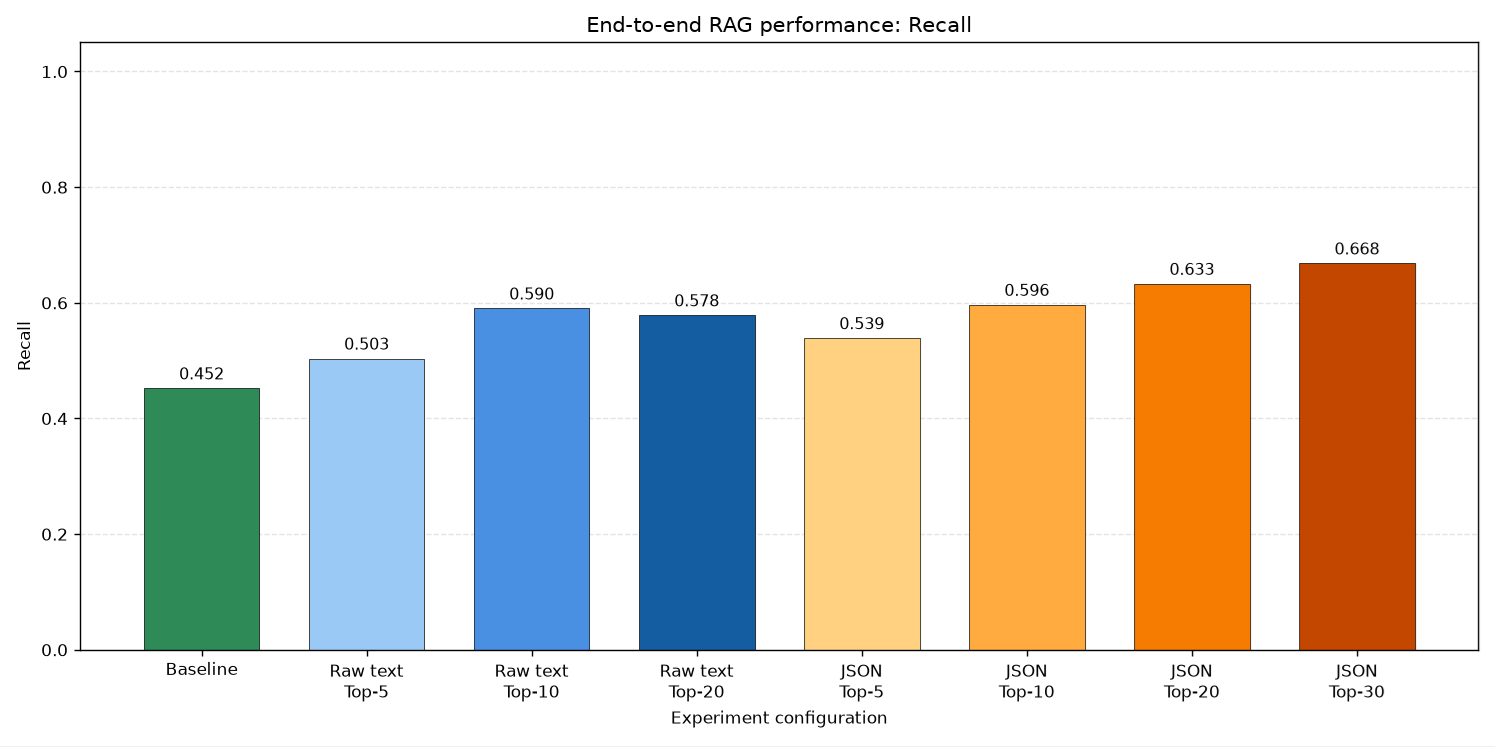
\includegraphics[width=\linewidth]{figures/overall_e2e_recall.png}
        \caption{Recall}
        \label{fig:overall_e2e_recall}
    \end{subfigure}

    \vspace{0.2cm}

    % Row 2: F1 and Exact Match
    \begin{subfigure}[t]{0.48\textwidth}
        \centering
        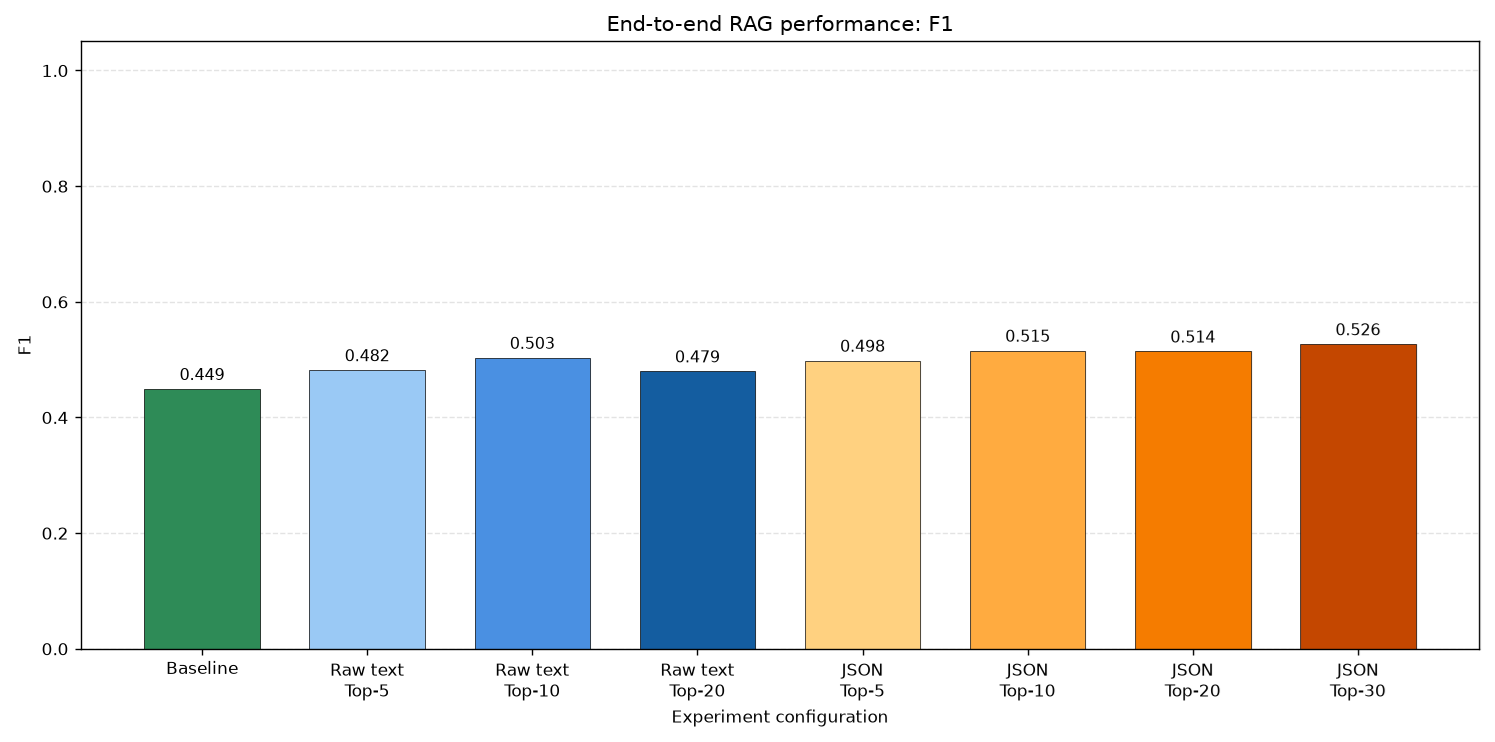
\includegraphics[width=\linewidth]{figures/overall_e2e_f1.png}
        \caption{F1 Score}
        \label{fig:overall_e2e_f1}
    \end{subfigure}
    \hfill
    \begin{subfigure}[t]{0.48\textwidth}
        \centering
        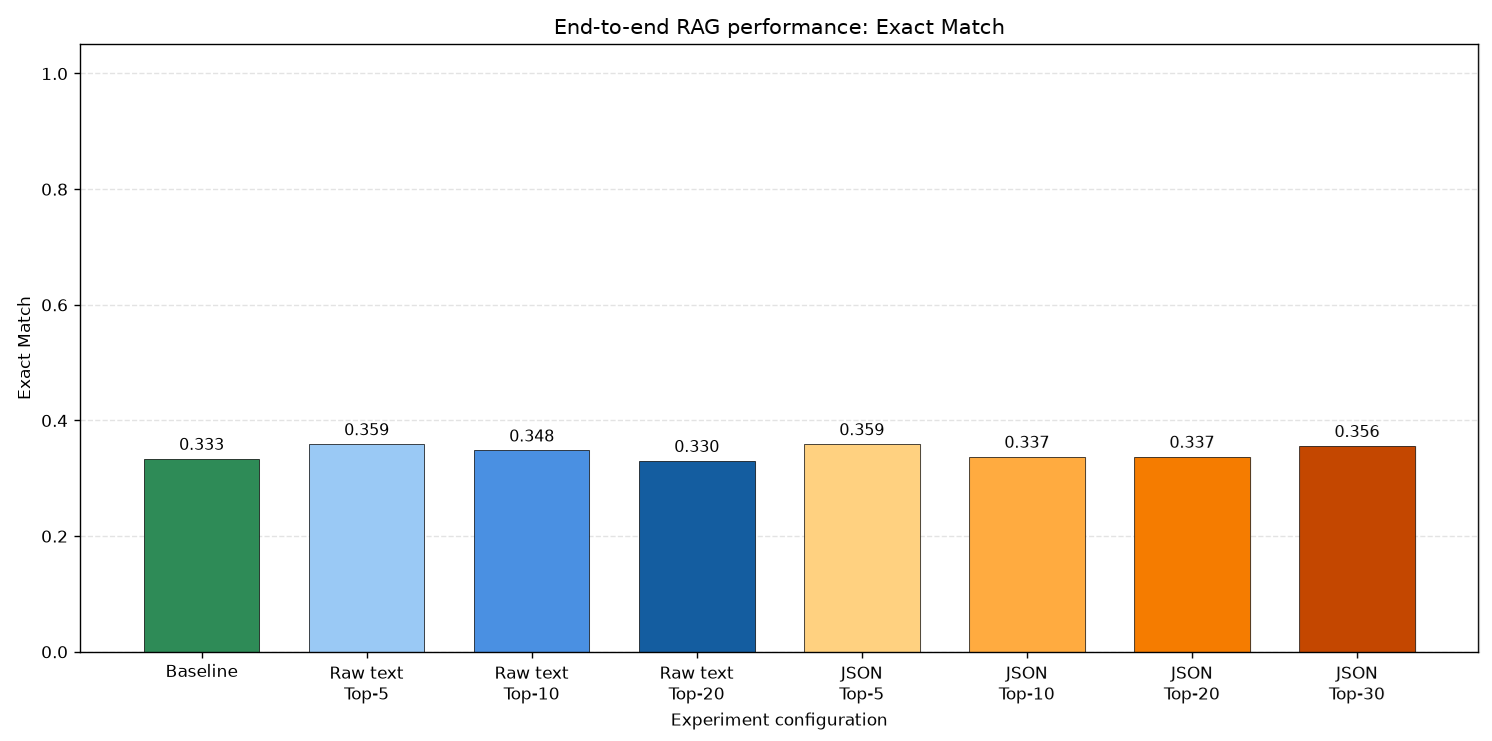
\includegraphics[width=\linewidth]{figures/overall_e2e_exact_match.png}
        \caption{Exact Match}
        \label{fig:overall_e2e_exact_match}
    \end{subfigure}

    \caption{Overall performance comparison of baseline, raw-text-augmented, and JSON-augmented configurations in the end-to-end RAG experiment across Precision, Recall, F1, and Exact Match, using different numbers of retrieved battles (top-k).}
    \label{fig:overall_e2e_comparison}
\end{figure}

\begin{table}[H]
    \centering
    \caption{Overall end-to-end generation performance across the baseline, raw-text-augmented, and JSON-augmented configurations with different top-$k$ context sizes}
    \label{tab:e2e_overall_performance}

    \scriptsize
    \renewcommand{\arraystretch}{1.5}
    \setlength{\tabcolsep}{3pt}

    \begin{tabular}{l c ccc cccc}
        \toprule
        & \multicolumn{1}{c}{\textbf{Baseline}}
        & \multicolumn{3}{c}{\textbf{Raw-text}}
        & \multicolumn{4}{c}{\textbf{JSON}} \\
        \cmidrule(lr){2-2}
        \cmidrule(lr){3-5}
        \cmidrule(lr){6-9}

        \textbf{Metric} &
        \textbf{Base} &
        \textbf{Top-5} &
        \textbf{Top-10} &
        \textbf{Top-20} &
        \textbf{Top-5} &
        \textbf{Top-10} &
        \textbf{Top-20} &
        \textbf{Top-30} \\
        \midrule

        \textbf{Precision} &
        0.467 &
        0.486 & 0.472 & 0.455 &
        0.486 & \textbf{0.499} & 0.482 & 0.494 \\

        \textbf{Recall} &
        0.452 &
        0.503 & 0.590 & 0.578 &
        0.539 & 0.596 & 0.633 & \textbf{0.668} \\

        \textbf{F1} &
        0.449 &
        0.482 & 0.503 & 0.479 &
        0.498 & 0.515 & 0.514 & \textbf{0.526} \\

        \textbf{Exact Match} &
        0.333 &
        \textbf{0.359} & 0.348 & 0.330 &
        \textbf{0.359} & 0.337 & 0.337 & 0.356 \\

        \bottomrule
    \end{tabular}

    \par\vspace{4pt}
    \begin{minipage}{\linewidth}
        \footnotesize
        \textit{Note:} Bold values indicate the best-performing
        configuration for each metric across all evaluated
        context sizes.
    \end{minipage}

\end{table}
For recall, the advantage of the structured JSON context is more visible. At \(k=10\), the JSON-augmented model achieved a recall of 0.596, compared with 0.452 for the baseline LLM and 0.590 for the raw-text-augmented model, corresponding to improvements of approximately 31.9\% and 1.0\%, respectively. When the context size was increased to 20 retrieved battles, JSON recall further improved to 0.633, representing an increase of approximately 40.0\% over the baseline LLM and 9.4\% over the raw-text-augmented model at the same context size. At the same time, JSON@20 also achieved higher precision than both the baseline LLM (+3.2\%) and raw-text@20 (+5.9\%).

Overall, in the complete RAG setting, structured JSON battle representations primarily improve the model’s ability to identify a larger proportion of relevant battles, while providing only modest gains in precision. Unlike in the Oracle-context experiment, the overall performance of the JSON-augmented model remains relatively close to the baseline LLM. This is likely because final answer quality in the end-to-end setting is additionally constrained by retrieval errors and by whether the relevant battles are present in the retrieved top-$k$ context.

In the subsequent experiments, we chose a context size of \(k = 20\), as it provided the best balance between recall and precision while also avoiding run errors for both the raw-text-augmented and JSON-augmented settings. Figure~\ref{fig:e2e_error_count_k} illustrates the relationship between the number of retrieved JSON battle records and the number of generation errors. No errors were observed for context sizes from \(k = 5\) to \(k = 20\). However, starting from \(k = 25\), generation failures began to appear and reached their highest number at \(k = 40\). These failures mainly included response parsing errors and generations that exceeded the maximum token limit.

\begin{figure}[!htbp]
    \centering
    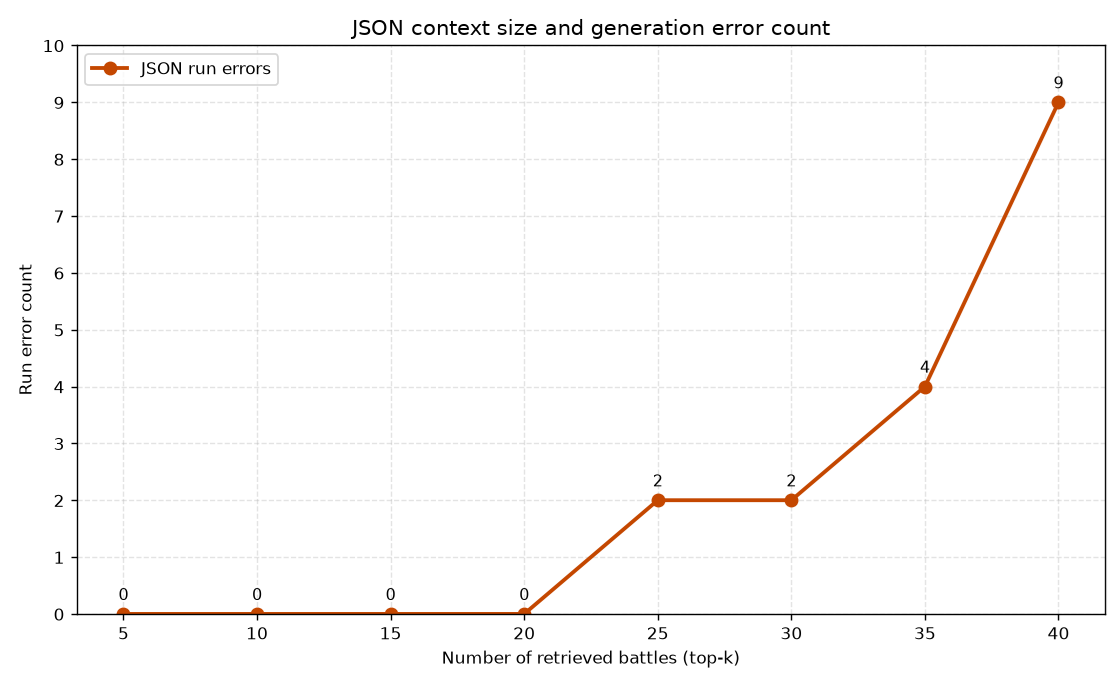
\includegraphics[
        width=0.90\textwidth,
        keepaspectratio
    ]{figures/e2e_error_count_k.png}
    \caption{Number of generation run errors in the JSON-augmented end-to-end RAG experiment as a function of the number of retrieved battle representations (top-$k$).}
    \label{fig:e2e_error_count_k}
\end{figure}

\subsection{Faithfulness and Context Relevance}
Faithfulness and context relevance were evaluated separately on the complete query set of 92 queries, excluding the Similarity query type. Figure~\ref{fig:json_top20_faithfulness} presents the faithfulness scores and evaluation configuration. Macro faithfulness, where each query receives equal weight, reaches 0.896, while micro faithfulness, where each evaluated statement receives equal weight, reaches 0.904. This means that 90.4\% of the evaluated statements were supported by the retrieved context. These results indicate that the JSON-augmented model largely relied on the retrieved context to generate factually grounded answers.

\begin{figure}[!htbp]
    \centering
    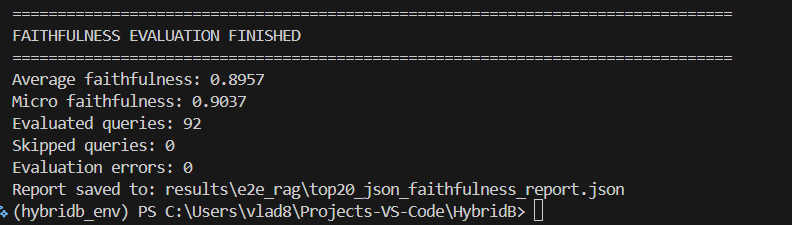
\includegraphics[
        width=0.90\textwidth,
        height=0.20\textheight,
        keepaspectratio
    ]{figures/json_top20_faithfulness.png}
    \caption{Faithfulness evaluation results for the JSON-augmented end-to-end RAG configuration with top-20 retrieved battle representations.}
    \label{fig:json_top20_faithfulness}
\end{figure}

Context relevance was evaluated for \(k = 5\), \(10\), and \(20\) to analyze how the amount of retrieved context affects the proportion of retrieved battle records that are actually relevant to answering the query. Table~\ref{tab:context_relevance} presents the context relevance results and evaluation configuration. Figure~\ref{fig:e2e_context_relevance_k} additionally visualizes the relationship between the number of retrieved battles and the average context relevance score. Particularly, it illustrates that as the number of retrieved battles increases, average context relevance steadily decreases, from 61.3\% at $k = 5$ to 49.5\% at $k = 20$. A context relevance score of 61\% indicates that, on average, approximately 61\% of the retrieved battle records contained information relevant to answering the corresponding query.

\begin{figure}[!htbp]
    \centering
    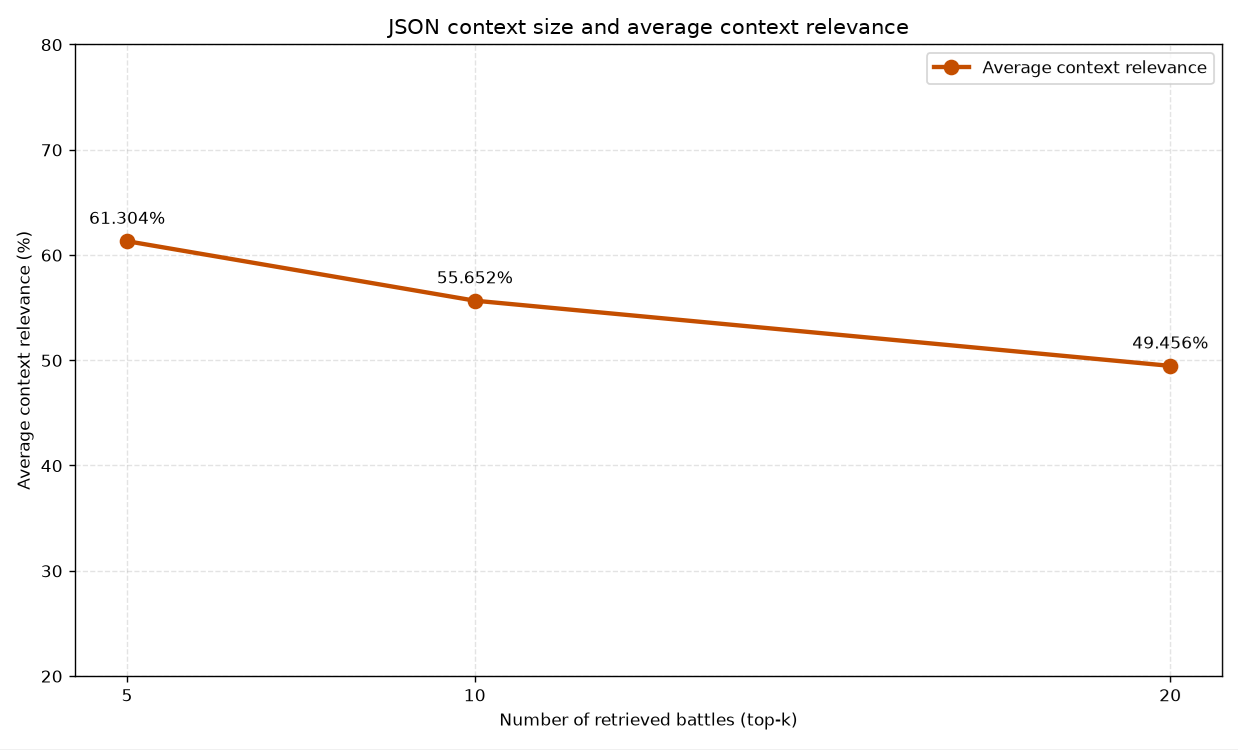
\includegraphics[
        width=0.80\textwidth,
        height=0.30\textheight,
        keepaspectratio
    ]{figures/e2e_context_relevance_k.png}
    \caption{Average context relevance in the JSON-augmented end-to-end RAG experiment as a function of the number of retrieved battle representations (top-k).}
    \label{fig:e2e_context_relevance_k}
\end{figure}

\begin{table}[H]
    \centering
    \caption{Context relevance results for different numbers of retrieved JSON battle records}
    \label{tab:context_relevance}

    \small
    \renewcommand{\arraystretch}{1.5}
    \setlength{\tabcolsep}{8pt}

    \begin{tabular}{c c c c c}
        \toprule
        \textbf{Top-$k$} &
        \shortstack{\textbf{Average Context}\\\textbf{Relevance}} &
        \textbf{Relevant Records} &
        \textbf{Total Context Records} &
        \textbf{Evaluation Errors} \\
        \midrule

        \textbf{5} &
        \textbf{61.304\%} &
        282 &
        460 &
        0 \\

        \textbf{10} &
        55.652\% &
        512 &
        920 &
        0 \\

        \textbf{20} &
        49.457\% &
        910 &
        1,840 &
        0 \\

        \bottomrule
    \end{tabular}

    \par\vspace{4pt}
    \begin{minipage}{\linewidth}
        \footnotesize
        \textit{Note:} Bold values indicate the highest average
        context relevance score.
    \end{minipage}

\end{table}

\subsection{End-to-end RAG Performance for Common and Rare Battles}
In the next sub-experiment, we assessed the performance of the complete pipeline separately for common- and rare-battle queries. We wanted to examine whether a similar trend would appear to the one observed in the Oracle-context generation experiment, where the augmented LLMs achieved substantial improvements over the baseline LLM for rare-battle queries. Table~\ref{tab:e2e_common_rare} represents the exact metric scores for the three model configurations across all four evaluation metrics.
\begin{table}[H]
    \centering
    \caption{End-to-end RAG performance for common and rare battle queries across baseline, raw-text-augmented, and JSON-augmented configurations}
    \label{tab:e2e_common_rare}

    \small
    \renewcommand{\arraystretch}{1.4}
    \setlength{\tabcolsep}{6pt}

    \begin{tabular}{l ccc ccc}
        \toprule
        & \multicolumn{3}{c}{\textbf{Common}}
        & \multicolumn{3}{c}{\textbf{Rare}} \\
        \cmidrule(lr){2-4}
        \cmidrule(lr){5-7}

        \textbf{Metric} &
        \textbf{Baseline} &
        \textbf{Raw text} &
        \textbf{JSON} &
        \textbf{Baseline} &
        \textbf{Raw text} &
        \textbf{JSON} \\
        \midrule

        \textbf{Precision} &
        \textbf{0.665} & 0.527 & 0.537 &
        0.137 & 0.413 & \textbf{0.416} \\

        \textbf{Recall} &
        0.629 & 0.605 & \textbf{0.663} &
        0.145 & 0.561 & \textbf{0.583} \\

        \textbf{F1} &
        \textbf{0.632} & 0.541 & 0.571 &
        0.140 & 0.440 & \textbf{0.452} \\

        \textbf{Exact Match} &
        \textbf{0.448} & 0.350 & 0.390 &
        0.129 & \textbf{0.333} & 0.312 \\

        \bottomrule
    \end{tabular}

    \par\vspace{4pt}
    \begin{minipage}{\linewidth}
        \footnotesize
        \textit{Note:} Bold values indicate the
        best-performing configuration for each metric
        within the corresponding query rarity group.
    \end{minipage}

\end{table}
As shown in Figure~\ref{fig:rarity_e2e_comparison}, for common-battle queries, the baseline LLM remains highly competitive and achieves the highest precision, F1, and exact-match scores, with values of 0.665, 0.632, and 0.448, respectively. The JSON-augmented model achieves the highest recall of 0.663, compared with 0.629 for the baseline LLM. However, its precision, F1, and exact-match scores remain lower than those of the baseline.

\begin{figure}[!htbp]
    \centering

    % Row 1: Precision and Recall
    \begin{subfigure}[t]{0.40\textwidth}
        \centering
        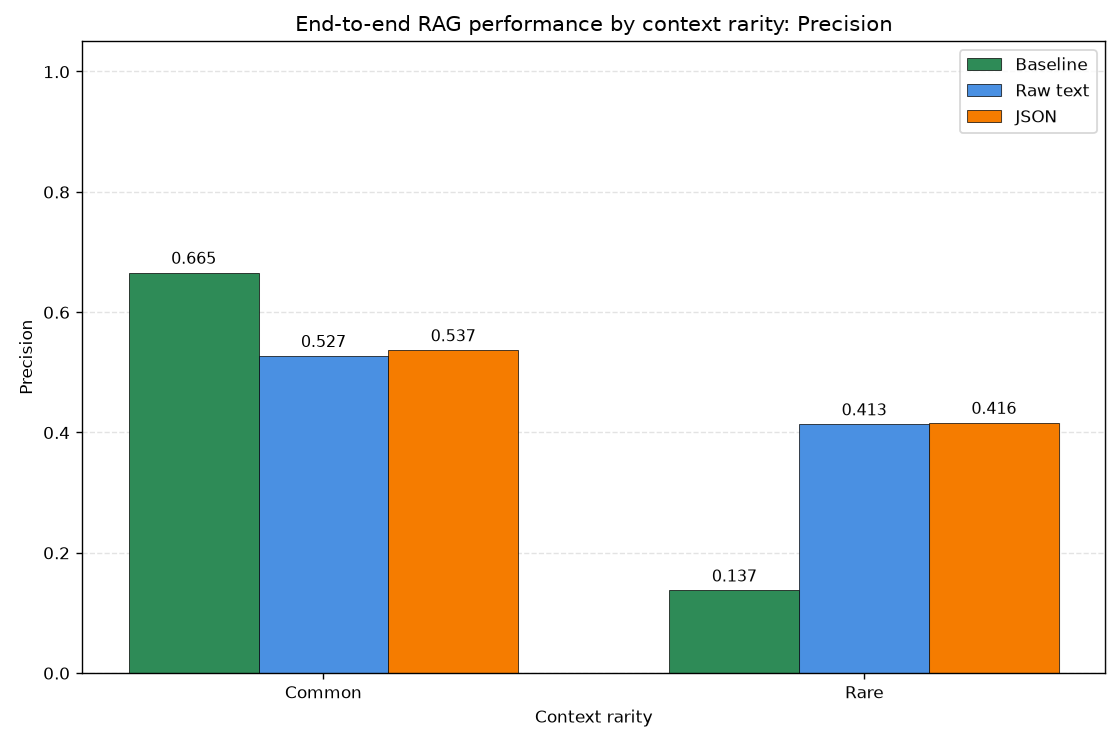
\includegraphics[width=\linewidth]{figures/rarity_e2e_precision.png}
        \caption{Precision}
        \label{fig:rarity_e2e_precision}
    \end{subfigure}
    \hfill
    \begin{subfigure}[t]{0.40\textwidth}
        \centering
        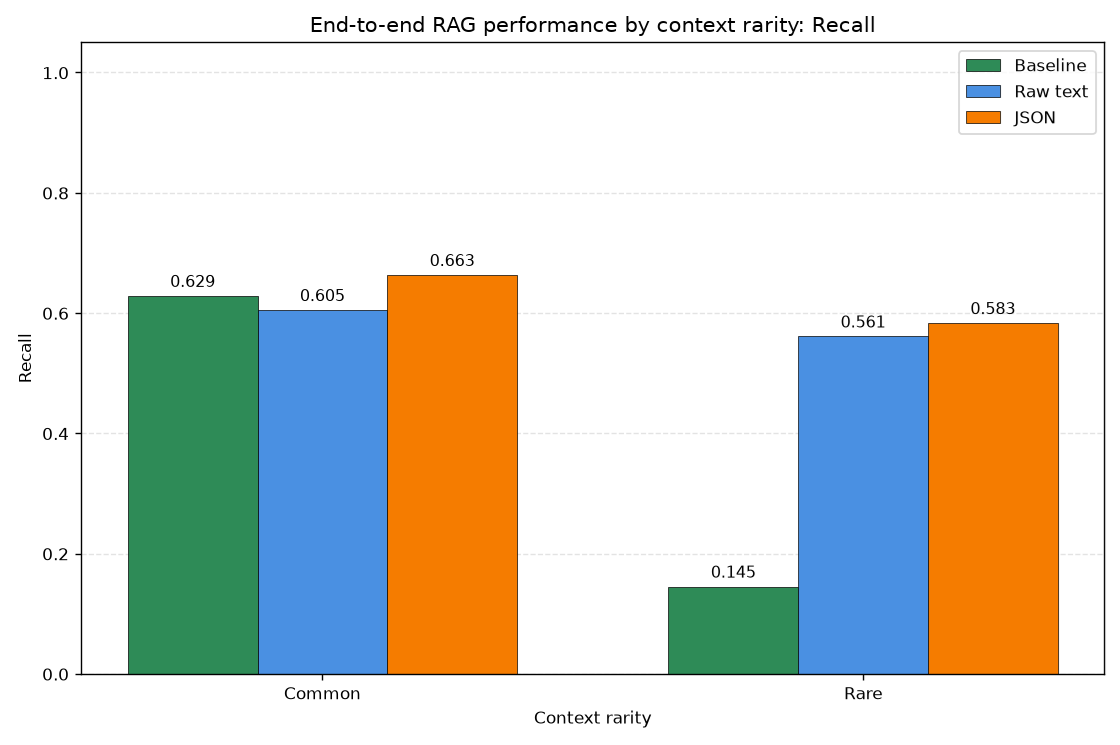
\includegraphics[width=\linewidth]{figures/rarity_e2e_recall.png}
        \caption{Recall}
        \label{fig:rarity_e2e_recall}
    \end{subfigure}

    \vspace{0.2cm}

    % Row 2: F1 and Exact Match
    \begin{subfigure}[t]{0.40\textwidth}
        \centering
        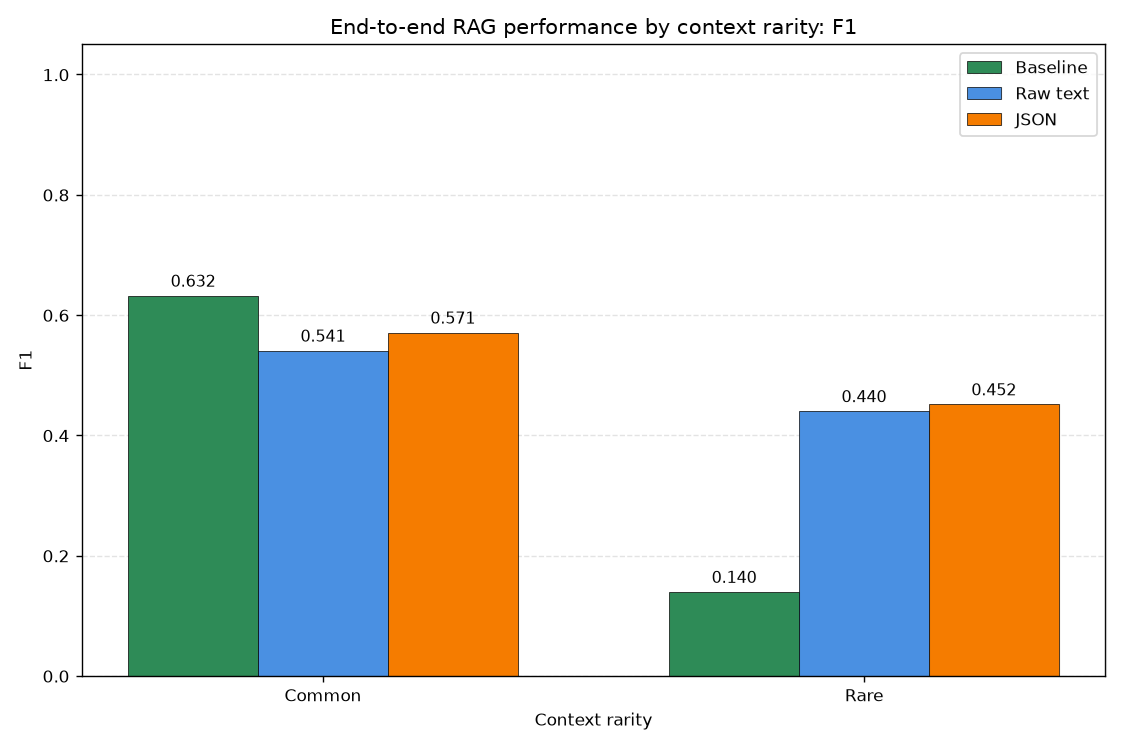
\includegraphics[width=\linewidth]{figures/rarity_e2e_f1.png}
        \caption{F1 Score}
        \label{fig:rarity_e2e_f1}
    \end{subfigure}
    \hfill
    \begin{subfigure}[t]{0.40\textwidth}
        \centering
        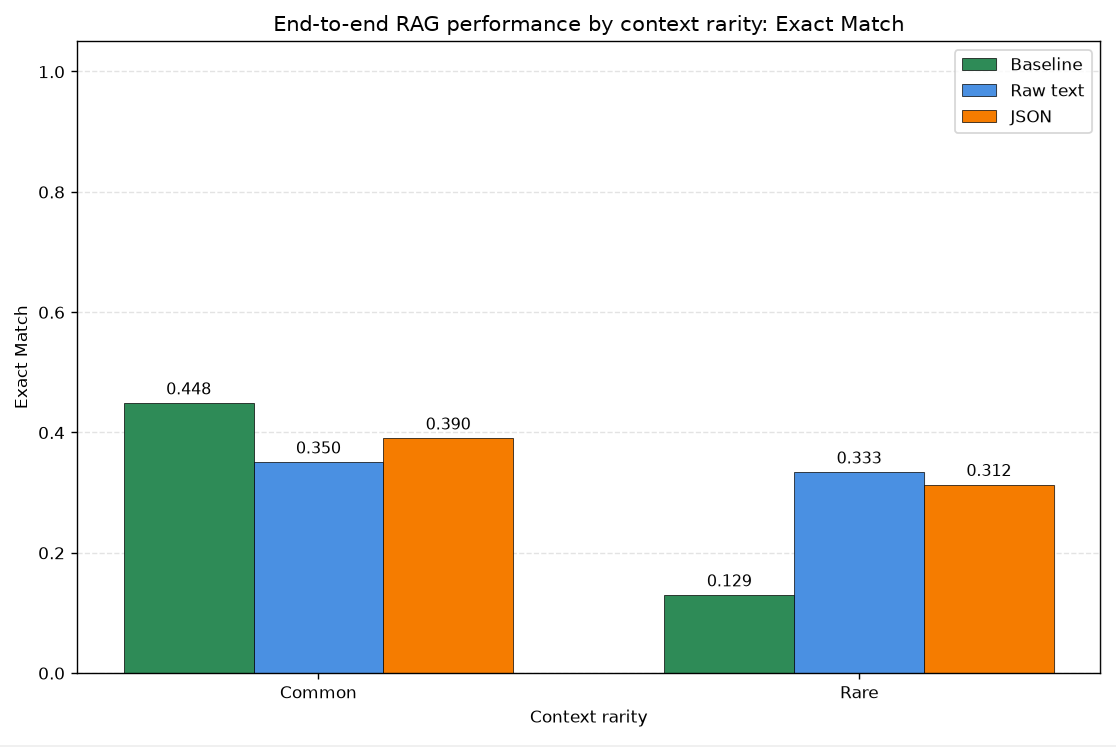
\includegraphics[width=\linewidth]{figures/rarity_e2e_exact_match.png}
        \caption{Exact Match}
        \label{fig:rarity_e2e_exact_match}
    \end{subfigure}

    \caption{Comparison of baseline, raw-text-augmented, and JSON-augmented configurations in the end-to-end RAG experiment across common and rare historical battle queries, evaluated using Precision, Recall, F1, and Exact Match.}
    \label{fig:rarity_e2e_comparison}
\end{figure}

Similar to the Oracle-context generation experiment, we observed a substantially different pattern for rare-battle queries. Both context-augmented models again strongly outperform the baseline LLM across all four evaluation metrics. The JSON-augmented model improves precision from 0.137 to 0.416 (+203.6\%), recall from 0.145 to 0.583 (+302.1\%), F1 from 0.140 to 0.452 (+222.9\%), and exact match from 0.129 to 0.312 (+141.9\%). This corresponds to an average relative improvement of approximately 217.6\% over the baseline. The raw-text-augmented model shows a similar pattern, improving precision to 0.413, recall to 0.561, F1 to 0.440, and exact match to 0.333, corresponding to an average relative improvement of approximately 215.2\% over the baseline.

Overall, the results show that external context provides only a limited benefit for common-battle queries, while it becomes substantially more helpful for rare-battle queries.
\subsection{End-to-end RAG Performance by Query Type}
Next, we evaluate the complete pipeline separately for each query type to examine whether its performance varies across different query categories. All metric results are provided in Table~\ref{tab:e2e_query_types_1}, Table~\ref{tab:e2e_query_types_2} and Table~\ref{tab:e2e_similarity}.
\begin{table}[H]
    \centering
    \caption{End-to-end RAG performance across Temporal, Spatial/Terrain, and Participant-related query types}
    \label{tab:e2e_query_types_1}

    \scriptsize
    \renewcommand{\arraystretch}{1.4}
    \setlength{\tabcolsep}{3pt}

    \begin{tabular}{l ccc ccc ccc}
        \toprule
        & \multicolumn{3}{c}{\textbf{Temporal}}
        & \multicolumn{3}{c}{\textbf{Spatial / Terrain}}
        & \multicolumn{3}{c}{\textbf{Participant-related}} \\
        \cmidrule(lr){2-4}
        \cmidrule(lr){5-7}
        \cmidrule(lr){8-10}

        \textbf{Metric} &
        \textbf{Baseline} & \textbf{Raw text} & \textbf{JSON} &
        \textbf{Baseline} & \textbf{Raw text} & \textbf{JSON} &
        \textbf{Baseline} & \textbf{Raw text} & \textbf{JSON} \\
        \midrule

        \textbf{Precision} &
        \textbf{1.000} & 0.833 & 0.823 &
        0.218 & 0.340 & \textbf{0.369} &
        0.572 & \textbf{0.592} & 0.562 \\

        \textbf{Recall} &
        0.887 & 0.887 & \textbf{0.900} &
        0.205 & 0.449 & \textbf{0.522} &
        0.520 & \textbf{0.833} & 0.828 \\

        \textbf{F1} &
        \textbf{0.917} & 0.832 & 0.809 &
        0.210 & 0.374 & \textbf{0.417} &
        0.535 & \textbf{0.641} & 0.614 \\

        \textbf{Exact Match} &
        \textbf{0.800} & 0.600 & 0.600 &
        0.182 & \textbf{0.231} & \textbf{0.231} &
        0.400 & \textbf{0.429} & 0.400 \\

        \bottomrule
    \end{tabular}

    \par\vspace{4pt}
    \begin{minipage}{\linewidth}
        \footnotesize
        \textit{Note:} Bold values indicate the best-performing
        configuration for each metric within the corresponding
        query type.
    \end{minipage}

\end{table}
\begin{table}[H]
    \centering
    \caption{End-to-end RAG performance across Narrative/Tactical, Outcome-related, and Weapon/Unit-related query types}
    \label{tab:e2e_query_types_2}

    \scriptsize
    \renewcommand{\arraystretch}{1.4}
    \setlength{\tabcolsep}{3pt}

    \begin{tabular}{l ccc ccc ccc}
        \toprule
        & \multicolumn{3}{c}{\textbf{Narrative / Tactical}}
        & \multicolumn{3}{c}{\textbf{Outcome-related}}
        & \multicolumn{3}{c}{\textbf{Weapon / Unit-related}} \\
        \cmidrule(lr){2-4}
        \cmidrule(lr){5-7}
        \cmidrule(lr){8-10}

        \textbf{Metric} &
        \textbf{Baseline} & \textbf{Raw text} & \textbf{JSON} &
        \textbf{Baseline} & \textbf{Raw text} & \textbf{JSON} &
        \textbf{Baseline} & \textbf{Raw text} & \textbf{JSON} \\
        \midrule

        \textbf{Precision} &
        0.295 & \textbf{0.443} & 0.341 &
        \textbf{0.425} & 0.358 & 0.393 &
        0.483 & \textbf{0.497} & 0.437 \\

        \textbf{Recall} &
        0.309 & \textbf{0.512} & 0.469 &
        0.425 & 0.394 & \textbf{0.465} &
        0.463 & \textbf{0.725} & 0.613 \\

        \textbf{F1} &
        0.298 & \textbf{0.456} & 0.372 &
        \textbf{0.424} & 0.353 & 0.415 &
        0.467 & \textbf{0.565} & 0.470 \\

        \textbf{Exact Match} &
        0.227 & \textbf{0.400} & 0.273 &
        \textbf{0.333} & 0.182 & \textbf{0.333} &
        \textbf{0.350} & 0.250 & 0.250 \\

        \bottomrule
    \end{tabular}

    \par\vspace{4pt}
    \begin{minipage}{\linewidth}
        \footnotesize
        \textit{Note:} Bold values indicate the best-performing
        configuration for each metric within the corresponding
        query type.
    \end{minipage}

\end{table}
\begin{table}[H]
    \centering
    \caption{End-to-end RAG performance for Similarity queries across baseline, raw-text-augmented, and JSON-augmented configurations}
    \label{tab:e2e_similarity}

    \small
    \renewcommand{\arraystretch}{1.4}
    \setlength{\tabcolsep}{12pt}

    \begin{tabular}{l ccc}
        \toprule
        & \multicolumn{3}{c}{\textbf{Similarity}} \\
        \cmidrule(lr){2-4}

        \textbf{Metric} &
        \textbf{Baseline} &
        \textbf{Raw text} &
        \textbf{JSON} \\
        \midrule

        \textbf{Precision} &
        \textbf{0.410} & 0.045 & 0.103 \\

        \textbf{Recall} &
        \textbf{0.490} & 0.070 & 0.170 \\

        \textbf{F1} &
        \textbf{0.426} & 0.053 & 0.107 \\

        \textbf{Exact Match} &
        \textbf{0.200} & 0.000 & 0.000 \\

        \bottomrule
    \end{tabular}

    \par\vspace{4pt}
    \begin{minipage}{0.85\textwidth}
        \footnotesize
        \textit{Note:} Bold values indicate the
        best-performing configuration for each metric.
    \end{minipage}

\end{table}
The query-type experiment shows that the effect of JSON augmentation varies considerably across different query categories. When the four evaluation metrics are averaged within each query type, the JSON-augmented model outperforms the baseline in four of the seven categories: Narrative/Tactical, Participant-related, Spatial/Terrain, and Weapon/Unit-related queries. The strongest improvement is observed for Spatial/Terrain queries, where the average score increases from 0.204 to 0.385, corresponding to a relative improvement of approximately 88.8\%. Narrative/Tactical queries improve by 28.9\% compared with the baseline model, while Participant-related queries show an 18.6\% increase in the average score. Weapon/Unit-related queries, on the other hand, show only a minor improvement of 0.4\%.

The main advantage of JSON augmentation is observed in the recall metric. Here, the JSON-augmented model achieves higher recall than the baseline in six of the seven query types. In particular, for Spatial/Terrain queries, the JSON-augmented model outperforms the baseline by 154.6\%, increasing recall from 0.205 to 0.522. A similar trend is observed for Participant-related queries, with a 59.2\% improvement over the baseline, followed by Narrative/Tactical queries with a 51.8\% improvement and Weapon/Unit-related queries with an improvement of approximately 32\%. These results indicate that structured context mainly improves the model’s ability to recover relevant battles; however, this advantage is not universal. Similarity queries represent a clear failure case, where recall decreases from 0.490 for the baseline model to 0.170 for the JSON-augmented model. A similar pattern is observed for F1, where the baseline model substantially outperforms the JSON-augmented LLM. Temporal queries, as shown in Figure 5.3.3.2, are also handled well by the baseline model, which achieves slightly better results than the augmented configurations.

Particularly interesting results are observed for the Similarity query type, as illustrated in Figure~\ref{fig:similarity_e2e_comparison}. The JSON-augmented model achieves substantially lower scores than the baseline LLM across all four evaluation metrics. Across precision, recall, and F1, the baseline LLM outperforms the JSON-augmented model by approximately 261\% on average, while exact match is 0.0 for the JSON-augmented model. During the analysis, we found that this poor performance is primarily related to failures at the retrieval stage. In five of the ten Similarity queries, none of the corresponding gold battles appeared within the top 20 retrieved records, which prevented the JSON-augmented model from producing a correct gold answer.

\begin{figure}[!htbp]
    \centering

    % Row 1: Precision and Recall
    \begin{subfigure}[t]{0.48\textwidth}
        \centering
        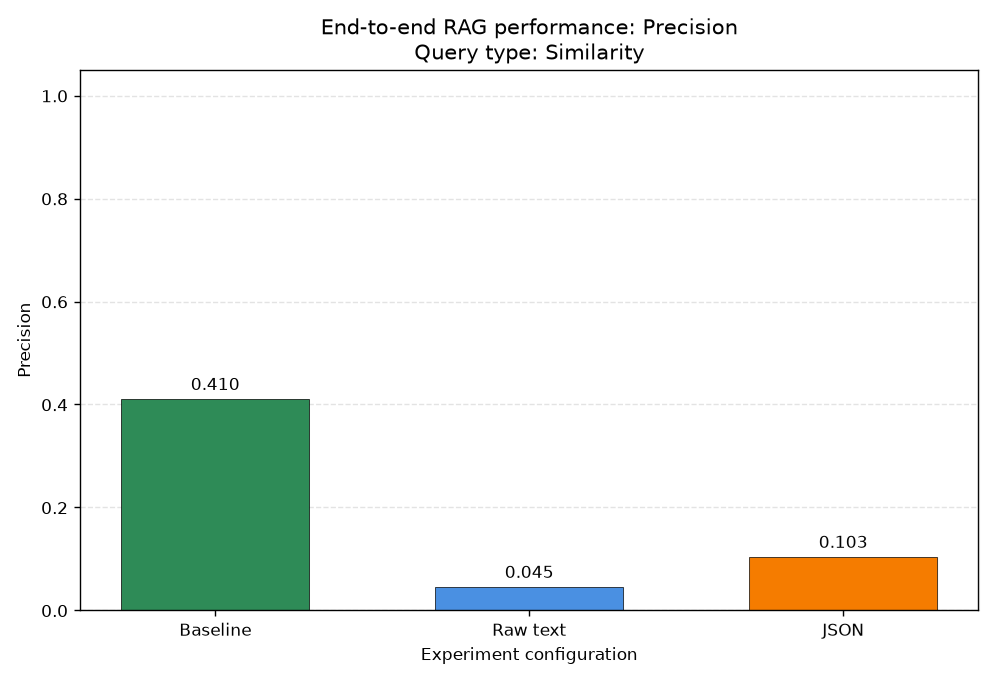
\includegraphics[width=\linewidth]{figures/similarity_e2e_precision.png}
        \caption{Precision}
        \label{fig:similarity_e2e_precision}
    \end{subfigure}
    \hfill
    \begin{subfigure}[t]{0.48\textwidth}
        \centering
        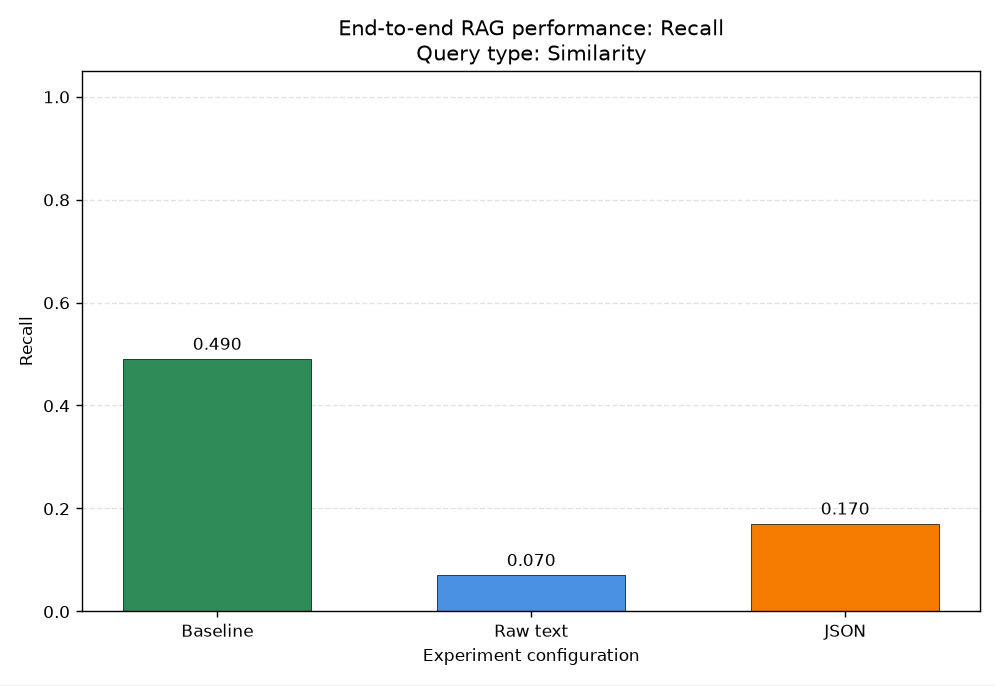
\includegraphics[width=\linewidth]{figures/similarity_e2e_recall.png}
        \caption{Recall}
        \label{fig:similarity_e2e_recall}
    \end{subfigure}

    \vspace{0.2cm}

    % Row 2: F1 and Exact Match
    \begin{subfigure}[t]{0.48\textwidth}
        \centering
        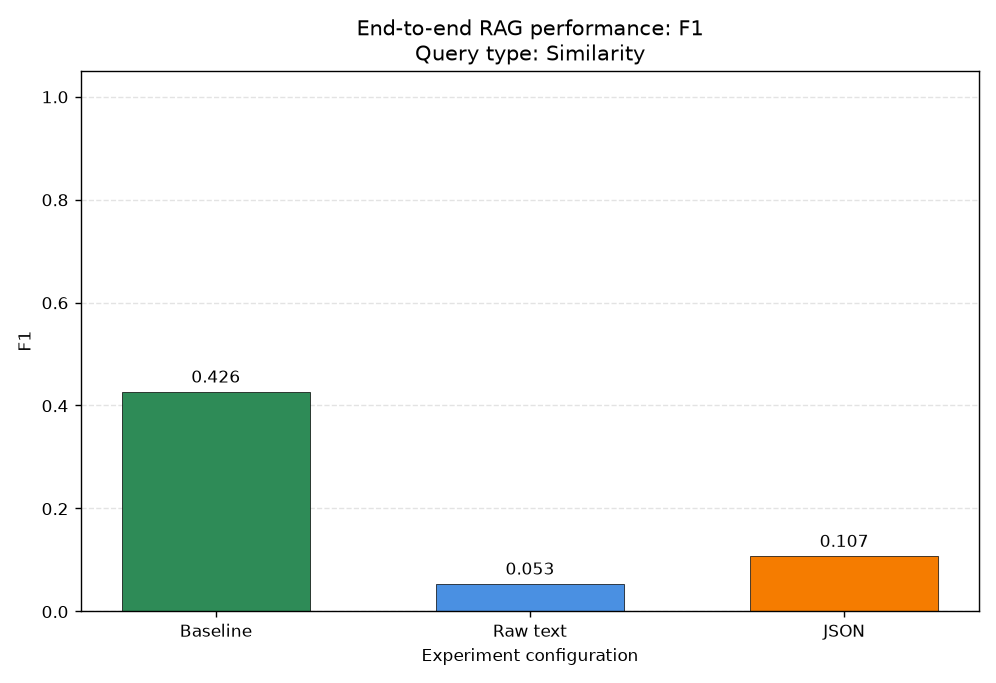
\includegraphics[width=\linewidth]{figures/similarity_e2e_f1.png}
        \caption{F1 Score}
        \label{fig:similarity_e2e_f1}
    \end{subfigure}
    \hfill
    \begin{subfigure}[t]{0.48\textwidth}
        \centering
        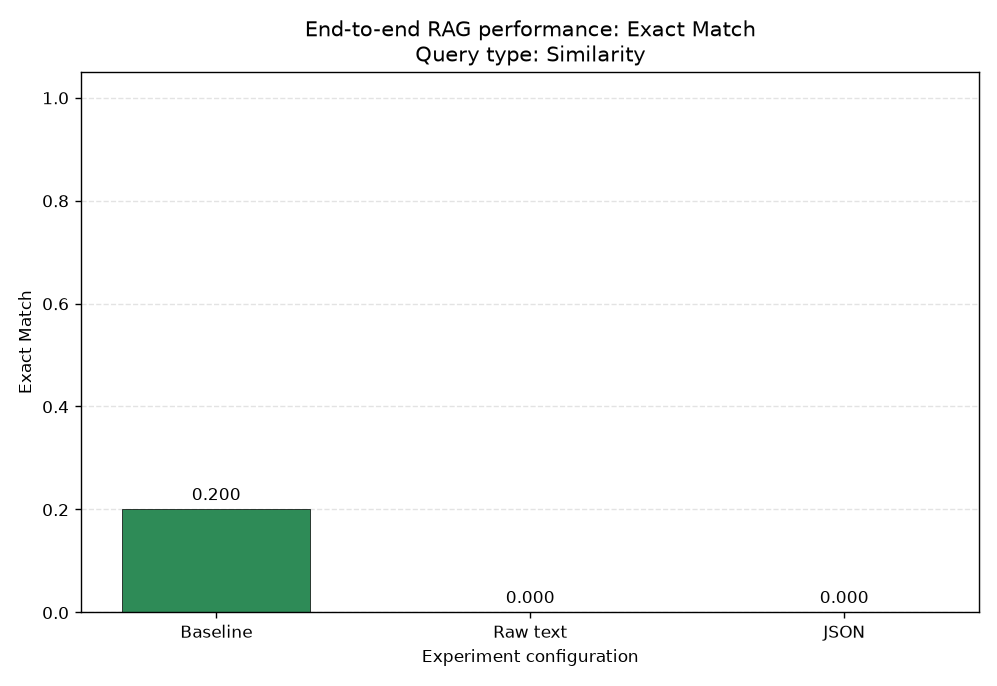
\includegraphics[width=\linewidth]{figures/similarity_e2e_exact_match.png}
        \caption{Exact Match}
        \label{fig:similarity_e2e_exact_match}
    \end{subfigure}

    \caption{Comparison of baseline, raw-text-augmented, and JSON-augmented configurations for Similarity queries in the end-to-end RAG experiment, evaluated using Precision, Recall, F1, and Exact Match.}
    \label{fig:similarity_e2e_comparison}
\end{figure}

A representative example is the first Similarity query: \textit{Find battles similar to Cannae in which encirclement or converging attacks trapped a large enemy force and led to catastrophic defeat.} The gold set contains the Battle of Tannenberg, the Battle of Stalingrad, the Battle of Kyiv (1941), and the Battle of Białystok–Minsk. However, the hybrid retrieval pipeline failed to retrieve any of these battles within the top 20 results. As illustrated in Table~\ref{tab:similarity_retrieval_failures}, the hybrid retrieval algorithm instead returned another semantically similar set of battles associated with encirclement and catastrophic defeat, including the Battle of Changping, the Battle of Lake Trasimene, the Battle of Walaja, and the Falaise Pocket. However, none of these battles belong to the predefined gold set. Consequently, the JSON-augmented model could not recover any gold battle from the provided context, resulting in a recall of 0 for this query.
\begin{table}[H]
    \centering
    \caption{Examples of retrieval failures for Similarity queries in the end-to-end RAG experiment}
    \label{tab:similarity_retrieval_failures}

    \small
    \renewcommand{\arraystretch}{1.5}
    \setlength{\tabcolsep}{4pt}

    \begin{tabular}{
        >{\raggedright\arraybackslash}p{0.17\textwidth}
        >{\raggedright\arraybackslash}p{0.25\textwidth}
        >{\centering\arraybackslash}p{0.10\textwidth}
        >{\raggedright\arraybackslash}p{0.25\textwidth}
        >{\centering\arraybackslash}p{0.10\textwidth}
    }
        \toprule
        \textbf{Query} &
        \textbf{Gold battles} &
        \textbf{Gold in top-20} &
        \textbf{Example retrieved alternatives} &
        \textbf{JSON Recall} \\
        \midrule

        q01 -- Similar to Cannae &
        Tannenberg, Stalingrad, Kiev, Bialystok--Minsk &
        \textbf{0/4} &
        Changping, Trasimene, Walaja, Falaise Pocket &
        0.000 \\
        \midrule

        q08 -- Similar to Stalingrad &
        Tannenberg &
        \textbf{0/1} &
        Kharkov, Korsun--Cherkassy, Demyansk, Kalach,
        Kiev, Vyazma &
        0.000 \\

        \bottomrule
    \end{tabular}
\end{table}
A similar pattern occurs for the q08 Similarity query, where the model was asked to find battles similar to Stalingrad in which an overextended attacking army was encircled by the enemy during a counteroffensive. The gold set contained only one battle, the Battle of Tannenberg, which was absent from the retrieved top-20 context. However, the hybrid retrieval pipeline still retrieved several plausible encirclement battles, including Korsun–Cherkassy, the Demyansk Pocket, Kalach, Kyiv, and the Vyazma Pocket.

These cases suggest an additional challenge in evaluating similarity-based queries. The previous query types were based on more explicit temporal, participant, spatial, weapon, or outcome constraints, whereas Similarity queries often involve several dimensions at once. As a result, different battles may be considered similar according to different properties. For example, q08 asks: \textit{Find a battle similar to Stalingrad in which an attacking army became overextended and was ultimately encircled by a large counteroffensive.} Similarity to Stalingrad may refer to encirclement, engagement scale, army size, or the broader counteroffensive narrative. This makes Similarity queries particularly sensitive to incomplete gold sets, since a retrieved battle may be semantically plausible even if it is not included in the predefined gold set. Consequently, retrieval and generation quality may be underestimated for this query type. This limitation of the query design is discussed further in Chapter 6, Discussion.

Overall, the query-type experiment shows that the usefulness of structured augmentation depends strongly on the semantic characteristics of each query type.
\chapter{Discussion}
In this chapter, we first summarize the key findings and draw the main conclusions. After that, we discuss the main limitations of our implemented RAG pipelines and present several directions for future work.
\section{Key Findings and Conclusions}
\subsection{Research Objective}
The main objective of this thesis was to investigate whether structured representations of historical battles can improve retrieval and LLM-based question answering in this domain. To address this objective, we designed a structured JSON representation schema that combines factual, military, temporal, spatial, participant-related, outcome-related, and narrative information. We then constructed a large-scale knowledge base containing 11,561 historical battle representations and implemented lexical, dense, and hybrid retrieval pipelines. Finally, we evaluated how structured battle context affects answer generation compared with direct LLM querying and raw-text augmentation.
\subsection{Answers to the Research Questions}
We investigated three research questions. RQ1 focused on how historical battles can be represented through a structured schema that captures factual, military, participant-related, narrative, and other relevant information about the battle. RQ2 explored three different retrieval pipelines, lexical, dense, and hybrid, and compared their performance to determine which approach is most suitable for the complete end-to-end RAG pipeline. Finally, RQ3 investigated how structured battle context affects LLM-based question-answering performance compared with direct LLM querying and raw-text augmentation.

Regarding RQ1, we built a JSON battle representation schema that covers the mentioned aspects of a historical battle and can support different types of questions.

Regarding RQ2, we compared lexical, dense, and hybrid retrieval approaches for identifying relevant battle representations in our local knowledge base. The retrieval experiments showed that hybrid retrieval provided the most robust performance across the experiments, although dense retrieval achieved higher results in several cases. Across our designed query set, hybrid retrieval outperformed lexical retrieval by around 21\% on average across the six evaluation metrics and achieved slightly better overall performance than dense retrieval. The advantage of dense retrieval was particularly visible when relevant battle representations used different terminology from the query. Query type also had a noticeable effect on performance. Dense retrieval performed especially well for Temporal queries, while hybrid retrieval achieved the highest scores for Spatial/Terrain and Weapon/Unit-related queries. Overall, hybrid retrieval consistently improved over the lexical algorithm by combining both lexical and semantic relevance signals. However, its advantage over dense retrieval depended more strongly on the characteristics and formulation of the query.

Regarding RQ3, we evaluated structured battle representations in both Oracle-context and end-to-end RAG settings. In the Oracle-context experiment, the JSON-augmented model clearly outperformed both the baseline LLM and raw-text augmentation, with an average improvement of approximately 17.9\% over the baseline and 6.8\% over raw text, while the advantage was especially strong for rare-battle queries. In the complete RAG setting, the improvement was more moderate because final performance also depended on retrieval quality. The JSON-augmented model mainly improved recall and again showed the strongest gains for rare battles, where it outperformed the baseline across all four metrics. Overall, structured battle representations improve LLM-based question answering, particularly for rare or underrepresented battles, but their effectiveness in the complete RAG pipeline remains strongly dependent on whether relevant battles are successfully retrieved.
\subsection{Overall Conclusion}
Overall, this thesis demonstrated that historical battles can be represented through a structured schema and organized into a large-scale knowledge base containing 11,561 battle instances. We evaluated how these structured representations affect both retrieval and answer-generation quality under different experimental settings. Across our benchmark of 102 queries, the structured battle knowledge base generally improved the ability of augmented LLMs to identify relevant battles compared with the baseline model, with particularly strong benefits observed for rare-battle queries. We also compared three retrieval strategies and found that hybrid retrieval, which combines BM25 and dense rankings, provides the most robust overall performance in many cases. This makes it especially useful for queries that require both exact lexical matching and semantic similarity. At the same time, the experiments revealed several limitations related to retrieval quality, benchmark construction, schema normalization, and knowledge base coverage, which provide clear directions for future work.
\section{Limitations and Future Work}
\subsection{Benchmark Grounding and Historical Validity}
This limitation concerns the potential difference between the source used to construct the benchmark, which in our case is primarily Wikipedia, and the knowledge available to the evaluated baseline LLM. The queries, gold battle sets, and structured battle representations were constructed mainly from raw-text Wikipedia articles. Therefore, the augmented models receive evidence originating from the same source on which the queries and gold sets were based. In contrast, the baseline LLM relies on parametric knowledge acquired during training. The exact composition of this training knowledge is unknown and cannot be reproduced in our experiments. Its knowledge may originate from different encyclopedias, websites, historical books, and other sources in which historical events may be described or interpreted differently from Wikipedia.

This issue is particularly relevant in the historical domain, where causal relationships, participant roles, and interpretations of decisive events may differ across sources. As a result, the baseline LLM may generate a historically plausible answer and identify battles that are relevant according to its internal knowledge, while still deviating from the predefined gold set. Such disagreement does not necessarily mean that the baseline answer is historically incorrect, but may instead reflect differences between historical sources and interpretations. Therefore, the reported evaluation results should primarily be interpreted as agreement with a Wikipedia-grounded benchmark rather than as a measure of absolute historical correctness.

A possible direction for future work would be to construct the local knowledge base, queries, and gold battle sets using multiple historical sources rather than relying primarily on Wikipedia. The resulting benchmark could then be manually reviewed by domain experts to verify the selected battles and reduce the influence of source-specific interpretations.
\subsection{Wikipedia Data Quality}
For our implementation, we use Wikipedia and Wikidata as a single source of truth for knowledge base construction, query and gold-set construction, and model augmentation with this knowledge. We consider this a limitation. The amount and quality of information available on Wikipedia vary considerably depending on the battle or historical event. Several obscure battles may contain only limited descriptions of tactics, narrative and event sequence, participants, and their roles. Besides, Wikipedia is collaboratively edited, and its content may be insufficiently verified, incomplete, or subject to later revision. As a result, our constructed battle representations may inherit inconsistencies and data gaps from Wikipedia.
\subsection{Limited Knowledge Base Coverage}
The next limitation is the insufficient coverage of our knowledge base. As previously discussed in the Methodology chapter, all battle instances extracted into our local knowledge base were associated with the Wikidata class battle (\texttt{Q178561}) and were retrieved using a SPARQL query that selected battles with a corresponding English Wikipedia page. This additional filter already reduced the number of battle instances from 18,655 to 11,561. Besides, Wikidata contains several additional military event classes that may also be useful to include in our knowledge base. As illustrated in Table~\ref{tab:wikidata_extension_classes}, these may include siege, military operation, armed conflict, or military campaign. Additionally, Wikidata contains subclasses of battle that may represent more specific battle types, such as naval or air battles. Therefore, future work could investigate additional Wikidata classes that may be suitable for inclusion in our knowledge base and incorporate the corresponding instances.
\begin{table}[H]
    \centering
    \caption{Potential Wikidata classes for extending the historical battle knowledge base}
    \label{tab:wikidata_extension_classes}

    \small
    \renewcommand{\arraystretch}{1.5}
    \setlength{\tabcolsep}{8pt}

    \begin{tabular}{l c r l}
        \toprule
        \textbf{Wikidata class} &
        \textbf{Wikidata ID} &
        \textbf{Approx. instances} &
        \textbf{Relevance for extension} \\
        \midrule

        Battle &
        Q178561 &
        18,655 &
        Currently used \\

        Siege &
        Q188055 &
        3,918 &
        High \\

        Military operation &
        Q645883 &
        3,093 &
        High \\

        Armed conflict &
        Q350604 &
        530 &
        Medium \\

        Military campaign &
        Q831663 &
        1,276 &
        Medium \\

        \bottomrule
    \end{tabular}
\end{table}
\subsection{Field-Aware Lexical Retrieval}
Our implemented lexical retrieval pipeline does not explicitly consider the internal structure of the JSON battle representations, including field names and values. Instead, it treats each document as a single flat sequence of tokens.

This can be problematic when the lexical retrieval procedure returns syntactically similar but semantically different battle records. For instance, Table~\ref{tab:semantic_relationship_example} shows that two records may contain the same keywords that also appear in the query \textit{Find battles where Napoleon defeated the Prussian Army}, while still expressing opposite relationships between the participants. The wording is syntactically similar, but the semantic direction of who defeated whom is different. In this case, BM25 may rank both records highly even though only one of them is actually relevant to the query.
\begin{table}[H]
    \centering
    \caption{Example illustrating the importance of semantic relationships in battle retrieval}
    \label{tab:semantic_relationship_example}

    \small
    \renewcommand{\arraystretch}{1.5}
    \setlength{\tabcolsep}{6pt}

    \begin{tabular}{
        >{\raggedright\arraybackslash}p{0.25\textwidth}
        >{\raggedright\arraybackslash}p{0.65\textwidth}
    }
        \toprule
        \textbf{Query / document} &
        \textbf{Text} \\
        \midrule

        \textbf{Query} &
        \textit{Find battles where Napoleon defeated the Prussian Army.} \\
        \midrule

        \textbf{Relevant record} &
        \textit{Napoleon's French army defeated the Prussian army in the battle.} \\
        \midrule

        \textbf{Non-relevant record} &
        \textit{The Prussian army defeated Napoleon's French army in the battle.} \\

        \bottomrule
    \end{tabular}
\end{table}
One potential extension to our pipeline would be to add query-dependent metadata filtering that analyzes the query formulation and makes lexical retrieval operate only on the relevant JSON fields. For example, a query asking about terrain could prioritize fields such as terrain and location, while queries asking about participant tactics could give more attention to the \texttt{narrative\_patterns} and \texttt{tactics} fields.

This solution could be further combined with field-aware BM25 scoring. Previous work on structured lexical retrieval has extended the BM25 algorithm by assigning different weights to different document fields. For example, this work proposed BM25E, building on BM25F, where term frequencies from different structural fields are weighted before being used by the BM25 scoring function \citep{lu2006fieldweighted}. We could adapt a similar approach and assign different weights to different JSON fields depending on the retrieval task.

One question that still remains is how the retrieval algorithm can recognize which query patterns it should look for when the query is expressed in natural language. Queries can be quite complex, and it may be difficult to identify which fields should be prioritized. For example, query q050 asks: \textit{Find a battle where elephants attacked first, infantry then became locked in combat, and returning cavalry finally struck the rear of the losing army.} Here, the lexical retrieval algorithm would need to consider participant information, event order, and unit types. Recognizing these requirements automatically may be difficult.

One potential solution would be to use an LLM to identify the relevant fields that the retrieval algorithm should then search. Another solution could be to use database-like queries in which the user explicitly refers to the relevant field names. For query q050, an example of such a formulation is shown in Listing~\ref{lst:elephant_tactical_query}. However, matching field names alone would still not be sufficient, since the field values also need to be normalized and comparable. This leads to the next limitation concerning field normalization.

\begin{minipage}{\textwidth}
\begin{lstlisting}[
    style=sqlstyle,
    caption={SQL-style representation of a complex historical battle query involving war elephants, cavalry flanking, and a specific sequence of tactical events.},
    label={lst:elephant_tactical_query}
]
SELECT battle
FROM battles
WHERE weapons_or_units CONTAINS 'war elephants'
  AND tactics CONTAINS 'cavalry flanking'
  AND event_sequence MATCHES (
      'elephant attack'
      THEN 'infantry engagement'
      THEN 'cavalry return'
      THEN 'rear attack'
  )
  AND cavalry_target = 'losing army'
  AND outcome = 'decisive defeat';
\end{lstlisting}
\end{minipage}

\subsection{Schema Normalization}
This limitation concerns the degree of normalization in our battle representation schema. Initially, we provided an empty JSON schema to the LLM filler model, but the model was not instructed to use predefined values for all fields. Instead, the model independently interprets each battle passage and may express semantically similar information using different terms. For example, outcome-related fields may contain values such as \texttt{decisive victory}, \texttt{successful defense}, \texttt{successful withdrawal}, or \texttt{defeat}, while the LLM may assign alternative formulations describing the same meaning. We consider this a limitation because it reduces consistency across battle representations and makes keyword filtering or rule-based queries more difficult. Lexical retrieval may also become less accurate because semantically similar battle aspects can be described using different terms, as shown in Table~\ref{tab:query_json_semantic_differences}.
\begin{table}[H]
    \centering
    \caption{Examples of semantic differences between query terms and alternative descriptions in JSON representations}
    \label{tab:query_json_semantic_differences}

    \small
    \renewcommand{\arraystretch}{1.4}
    \setlength{\tabcolsep}{6pt}

    \begin{tabular}{
        >{\raggedright\arraybackslash}p{0.36\textwidth}
        >{\raggedright\arraybackslash}p{0.54\textwidth}
    }
        \toprule
        \textbf{Query term} &
        \textbf{Alternative description in JSON} \\
        \midrule

        Cavalry flanking maneuver &
        Mounted troops attacked from the side \\
        \midrule

        Decisive victory &
        Overwhelming defeat of the opposing army \\
        \midrule

        Retreat &
        Withdrawal from the battlefield \\
        \midrule

        Ambush &
        Surprise attack from a concealed position \\
        \midrule

        Defensive formation &
        Troops established a protective line \\
        \midrule

        River crossing &
        Army advanced across a waterway \\
        \midrule

        Encirclement &
        Enemy forces were surrounded \\
        \midrule

        Reinforcements arrived &
        Additional troops joined the battle \\

        \bottomrule
    \end{tabular}
\end{table}
Future versions of the representation schema could introduce a predefined set of labels that the LLM is instructed to use during the filling procedure, while still allowing free-text values where necessary. This could further improve consistency across battle representations and, consequently, retrieval performance.
\subsection{Query Set Construction}
The construction of the query set also introduces several limitations. First, it would be preferable for the generated queries and the corresponding gold battle sets to be manually verified against reliable historical sources to ensure that all relevant battles are included in the gold set and that the questions are formulated correctly, reducing the risk of potential misinterpretation. Another limitation concerns the batch-wise query construction procedure. Queries were generated using GPT-5.6 Sol from subsets of approximately 1,000 battle instances at a time. This means that the model could only consider potential gold battles available within the current batch and could miss relevant battles from other batches across the complete set of 11,561 prepared instances. This limitation is especially important for Similarity queries, where identifying similar battles may require awareness of the complete battle set. Therefore, semantically reasonable answers produced by the baseline model during our experiments may still be counted as false positives when they include relevant battles that fall outside the predefined gold set. Poor performance on Similarity queries should therefore be interpreted as a combination of retrieval failures and potentially incomplete gold labels, rather than purely as a generation failure of the augmented models.



\bibliographystyle{template/acl_natbib}
\bibliography{references}